% Use the "Thesis" style, based on the ECS Thesis style by Steve Gunn
\documentclass[a4paper, 11pt, oneside]{Thesis}
\pdfminorversion=5 % stop pdflatex worrying about 1.5 version pdfs
\graphicspath{{Figures/}} % Location of the graphics files (set up for graphics to be in PDF format)
\usepackage[utf8]{inputenc} %useful to type directly accentuated characters undefined method `context' for nil:NilClass

% For source code
\newenvironment{mytinylisting}
{\begin{list}{}{\setlength{\leftmargin}{1em}}\item\tiny\bfseries}
{\end{list}}

\hypersetup{
    colorlinks,
    citecolor=black,
    filecolor=black,
    linkcolor=black,
    urlcolor=black
}

\usepackage{lscape}
\usepackage{verbatim}
\usepackage{float} % for [H]ere
\usepackage{vector}
\usepackage{multirow}
\usepackage{graphicx}
\usepackage{subfigure}
\usepackage{rotating}
\usepackage{sectsty}
\usepackage{arydshln} % for dashed rules in tables
\usepackage{url}
\usepackage{algorithmic}
\usepackage{algorithm}
\usepackage{booktabs}
\usepackage{amsmath}
\usepackage{threeparttable}
\usepackage[table]{xcolor}
\definecolor{tableShade}{HTML}{F1F5FA}
%\usepackage[square, authoryear]{natbib}
\usepackage[sort&compress]{natbib}
% \usepackage{lineno}
% \linenumbers
\usepackage{arabtex}
\allsectionsfont{\sffamily}
%\renewcommand\familydefault{cmss}


\renewcommand{\textfraction}{0.05}
\renewcommand{\topfraction}{0.95}
\renewcommand{\bottomfraction}{0.95}
\renewcommand{\floatpagefraction}{0.35}
\setcounter{totalnumber}{5}


%% ----------------------------------------------------------------
\begin{document}

\frontmatter  % Begin Roman style (i, ii, iii, iv...) page numbering

\title  {Dissecting genetic interactions in complex traits}
\authors  {\texorpdfstring
           {\href{gib.hemani@roslin.ed.ac.uk}{Gibran Hemani}}
           {Author Name}
           }
\addresses  {\groupname\\\deptname\\\univname}
\date{\today}
\subject{}
\keywords{}
\maketitle

\setstretch{1.6}

% Define the page headers using the FancyHdr package and set up for one-sided printing
\fancyhead{}  % Clears all page headers and footers
\rhead{\thepage}
\lhead{}

\pagestyle{fancy}

\Declaration{
I, Gibran Hemani, declare that this thesis titled, `Dissecting genetic interactions in complex traits' and the work presented in it are my own. I confirm that:

\begin{itemize}
\item[\tiny{$\blacksquare$}] No part of this thesis has previously been submitted for a degree or any other qualification at this University or any other institution.

\item[\tiny{$\blacksquare$}] Where I have consulted the published work of others, this is always clearly attributed.

\item[\tiny{$\blacksquare$}] Where I have quoted from the work of others, the source is always given. With the exception of such quotations, this thesis is entirely my own work.

\item[\tiny{$\blacksquare$}] I have acknowledged all main sources of help.

\item[\tiny{$\blacksquare$}] Where the thesis is based on work done by myself jointly with others, I have made clear exactly what was done by others and what I have contributed myself.
\\
\end{itemize}


Signed:\\
\rule[1em]{25em}{0.5pt}

Date:\\
\rule[1em]{25em}{0.5pt}
}
\clearpage



\pagestyle{empty}  % No headers or footers for the following pages
\null\vfill
\textit{``For every complex problem there is a solution that is simple, neat, and wrong.''}
\begin{flushright}
H. L. Mencken
\end{flushright}
\vfill\vfill\vfill\vfill\vfill\vfill\null
\clearpage


\addtotoc{Abstract}
\setstretch{1}  
\abstract{\small{
Of central importance in the dissection of the components that govern complex traits is understanding the architecture of natural genetic variation. Genetic interaction, or epistasis, constitutes one aspect of this, but epistatic analysis has been largely avoided in genome wide association studies because of statistical and computational difficulties. This thesis explores both issues in the context of two-locus interactions.

Initially, through simulation and deterministic calculations it was demonstrated that not only can epistasis maintain deleterious mutations at intermediate frequencies when under selection, but that it may also have a role in the maintenance of additive variance. Based on the epistatic patterns that are evolutionarily persistent, and the frequencies at which they are maintained, it was shown that exhaustive two dimensional search strategies are the most powerful approaches for uncovering both additive variance and the other genetic variance components that are co-precipitated.

However, while these simulations demonstrate encouraging statistical benefits, two dimensional searches are often computationally prohibitive, particularly with the marker densities and sample sizes that are typical of genome wide association studies. To address this issue different software implementations were developed to parallelise the two dimensional triangular search grid across various types of high performance computing hardware. Of these, particularly effective was using the massively-multi-core architecture of consumer level graphics cards. While the performance will continue to improve as hardware improves, at the time of testing the speed was 2-3 orders of magnitude faster than CPU based software solutions that are in current use.

Not only does this software enable epistatic scans to be performed routinely at minimal cost, but it is now feasible to empirically explore the false discovery rates introduced by the high dimensionality of multiple testing. Through permutation analysis it was shown that the significance threshold for epistatic searches is a function of both marker density and population sample size, and that because of the correlation structure that exists between tests the threshold estimates currently used are overly stringent.

Although the relaxed threshold estimates constitute an improvement in the power of two dimensional searches, detection is still most likely limited to relatively large genetic effects. Through direct calculation it was shown that, in contrast to the additive case where the decay of estimated genetic variance was proportional to falling linkage disequilibrium between causal variants and observed markers, for epistasis this decay was exponential. One way to rescue poorly captured causal variants is to parameterise association tests using haplotypes rather than single markers. A novel statistical method that uses a regularised parameter selection procedure on two locus haplotypes was developed, and through extensive simulations it can be shown that it delivers a substantial gain in power over single marker based tests.

Ultimately, this thesis seeks to demonstrate that many of the obstacles in epistatic analysis can be ameliorated, and with the current abundance of genomic data gathered by the scientific community direct search may be a viable method to qualify the importance of epistasis.
}}
\clearpage


\acknowledgements{

For the duration of my studies I have received support, direction and inspiration from many people, and expressing the depth of my gratitude to them is proving to be an intractable problem.

My thanks to:\\
Chris Haley and Sara Knott, who gave me the opportunity to do this work, were extremely generous with their time, and offered advice, wisdom, and perspective;\\
John Woolliams, whose guidance was invaluable;\\
Ricardo Pong-Wong, who I have asked for help one thousand times and he has never been too busy;\\
Thanasis Theocharidis, Wenhua Wei, and Ian Handel, with whom I could talk about things that nobody else would talk to me about (computers);\\
the mysterious keepers of {\tt eddie} and {\tt cseht};\\
BBSRC, The Roslin Institute, Biosciences KTN, and Archie Clutter for the funding;\\
my friends, because you are all very distracting;\\
my family: Arman, Noor, and my wonderful parents.


%My advisers are pretty cool even though they are married and so thanks a lot. Also Ricardo. And my family, especially Arman for drinking coffee so I don't have to. I'd also like to acknowledge the city of Edinburgh for being so grey all the time and encouraging me to get my work done. And my computers for not crashing too much. And the large number of people that allow nettles to grow around here so that I have something to eat.  Thanks.

}

\clearpage



\setstretch{1}
\lhead{\emph{List of Publications}}
\listofpublications
{
Hemani G, Knott SA, Haley CS.\\
\textbf{An evolutionary perspective on epistasis and the missing heritability}.\\
In preparation. \\[.3cm]
Hemani G, Knott SA, Haley CS.\\
\textbf{Improvements in the power to detect epistasis through the use of haplotypes}.\\
In preparation. \\[.3cm]
Hemani G, Haley CS.\\
\textbf{Empirical estimates of significance thresholds for genome-wide searches for epistasis}.\\
In preparation. \\[.3cm]
French AT, Ogden R, Eland C, Hemani G, Pong-Wong R, Corcoran B, Summers KM.\\
\textbf{Genome-wide analysis of mitral valve disease in Cavalier King Charles Spaniels}.\\
Under submission. \\[.3cm]
Theocharidis A, Hemani G, Kargas M, Freeman T.\\
\textbf{A comparison of CPU and OpenCL parallelization methods for correlation and graph layout algorithms used in the network analysis of high dimensional data}.\\
Under submission. \\[.3cm]
Wei W, Hemani G, Hicks AA, Vitart V, Cabrera-Cardenas C, Navarro P, Huffman J, Hayward C, Knott SA, Rudan I, Pramstaller PP, Wild SH, Wilson JF, Campbell H, Hastie N, Wright AF, Haley CS.\\
\textbf{Characterisation of genome-wide association epistasis signals for serum uric acid in human population isolates.} \\
\emph{PLoS One} (2011) \emph{In press}. \\[.3cm]
Hemani G, Theocharidis A, Wei W, Haley CS.\\
\textbf{EpiGPU: exhaustive pairwise epistasis scans parallelized on consumer level graphics cards}.\\
\emph{Bioinformatics} (2011) 27 (11): 1462-1465. \\[.3cm]
Hadjipavlou G, Hemani G, Leach R, Louro B, Nadaf J, Rowe S, de Koning DJ.\\
\textbf{Extensive QTL and association analyses of the QTLMAS 2009 Data}.\\
\emph{BMC Proceedings} (2010) 4:S1 11. \\[.3cm]
}

\setstretch{1.6}


\lhead{\emph{Contents}}
\setcounter{tocdepth}{2}
\tableofcontents

\lhead{\emph{List of Figures}}
\listoffigures


\lhead{\emph{List of Tables}}
\listoftables


\setstretch{1.4}
\clearpage
\lhead{\emph{Symbols}}
\listofnomenclature{ll}
{
%\textbf{SNP} & \textbf{S}ingle \textbf{N}ucleotide \textbf{P}olymorphism \\
%\textbf{GWAS} & \textbf{G}enome \textbf{W}ide \textbf{A}ssociation \textbf{S}tudy \\
%\textbf{QTL} & \textbf{Q}uantitative \textbf{T}rait \textbf{L}ocus \\
%\textbf{GP map} & \textbf{G}enotype-\textbf{P}henotype map \\
%\textbf{LD} & \textbf{L}inkage \textbf{D}isequilibrium \\
%\textbf{CPU} & \textbf{C}entral \textbf{P}rocessing \textbf{U}nit \\
%\textbf{GPU} & \textbf{G}raphics \textbf{P}rocessing \textbf{U}nit \\
%\textbf{GPGPU} & \textbf{G}eneral \textbf{P}urpose \textbf{G}raphics \textbf{P}rocessing \textbf{U}nit \\
%\textbf{OLS} & \textbf{O}rdinary \textbf{L}east \textbf{S}quares \\
%\textbf{LASSO} & \textbf{L}east \textbf{A}bsolute \textbf{S}hrinkage and \textbf{S}election \textbf{O}perator \\
%\textbf{REML} & \textbf{RE}stricted \textbf{M}aximum \textbf{L}ikelihood \\
%\textbf{ROCK} & \textbf{RO}bust \textbf{C}lustering using lin\textbf{K}s \\
%\\
%$H^2$ & Broad-sense heritability \\
%$h^2$ & Narrow-sense heritability \\
%$r^2$ & Correlation coefficient \\
$x := y$ & $x$ changes to $y$\\
$\cap$ & Logical AND \\
$\cup$ & Logical OR \\
$| x |$ & Absolute value of $x$ \\
$\lceil x \rceil$ & Round $x$ up to the next integer \\
$\lfloor x \rfloor$ & Round $x$ down \\
$O(...)$ & Time complexity of an algorithm \\
}
\clearpage


\setstretch{1.6}
\mainmatter

\pagestyle{fancy}

% Introduction

\chapter{General introduction}
\label{Introduction}
\lhead{General introduction}

A fundamental objective of genetics is to forge a connection between phenotype and genotype. But with the complexity that ubiquitously governs biological systems this can be a daunting task, and it could be argued that the biggest failure in biological sciences over the past decade has been in the mapping of phenotypic variation to variation in the genome. This has prompted much debate regarding the fundamental nature of genetic variation, a question of crucial importance to the advancement of many fields such as medicine, animal and crop breeding, and evolutionary theory. This thesis seeks to develop novel methods for the detection of genetic variation that impact phenotypes with a particular emphasis on mapping interacting genetic factors. In this chapter the current understanding of the architecture of genetic variation is discussed, following a brief introduction of the historical paths that lead to today's practices in quantitative genetics.


\section{Historical foundations}

Prior to the rediscovery of Mendel's theory of genetic inheritance in 1900, there existed a division in the scientific community regarding the nature of evolution and the mechanisms that governed natural variation. Darwin's \emph{The Origin of Species} (1859) is celebrated today for first describing the mode of evolution in terms of natural selection, and creating the framework for the ``gradualist" school of thought, but it was not immediately accepted, and the emergence of several other major concepts were required before these ideas would eventually become solvent. At the time the alternative view was that evolutionary changes occurred not continuously but in discrete steps, and this ``saltatory" theory was often the more popular school of thought. Perhaps the biggest scientific criticism of gradualism was that it was incompatible with the then prevailing understanding of the transmission of hereditary material, blending inheritance. Under the theory of blending the variance of a character would disappear by a factor of a half each generation thus eventually insufficient variation would remain for gradual selection to act upon. In contrast, proponents of saltation were largely supported by cases from botanists and horticulturalists who often observed the sudden origin of deviant types in crops in agriculture. 

Post rediscovery of Mendelism, for a time the acrimony actually only deepened. The particulate nature of genetic material was intuitively appealing to the saltatory perspective, and for a time it was a common position to believe that Mendelism had destroyed Darwinism. It was not until the mathematical treatment of Mendelian inheritance in populations was developed through the Hardy-Weinberg principle in 1908 \citep{Hardy1908, Weinberg1908} that the theories of Mendelism and Darwinism were reconciled. It demonstrated that excluding any external forces, namely selection, the transmission of genetic variance through generations was shown to be stable - that is to say that the expected frequencies of neutral alleles for the next generation are equal to the observed frequencies in the current generation. As such, the criticisms applied to Darwinism in the context of blending inheritance were no longer pertinent under Mendelian inheritance, because genetic variation will be maintained. Buttressing the gradualism paradigm was the proposal of the infinitesimal paradigm \citep{Fisher1918}, which modelled adaptation on the assumption that mutations with large effects would likely be deleterious and thus rapidly purged from the population, and that adaptation occurred through the action of innumerable minute effects.

Still today the maintenance of genetic variation is not fully understood, and the evolutionary perspective of saltation, now more commonly referred to as punctuated equilibrium, has not been resolved. But the generic mechanism that underlies the relationship between genotype and phenotype had been established fairly convincingly and the foundations for population and quantitative genetics had been laid. The next section will follow the progress that has led from identifying the first molecular markers for genetic variation, to the situation today where whole genomes are being sequenced.


\section{Genetic variation}

The human genome comprises approximately three billion base pairs but surprisingly, with current predictions for the total number of genes at 20-25 thousand, only 1.5\% of this encodes for proteins \citep{InternationalHumanGenomeSequencingConsortium2004}. Estimates for the total proportion of the genome that is functional vary, but generally remain extremely low with comparative analysis suggesting a range of only 2.5 - 5\% \citep{Waterston2002, Chiaromonte2003, Lunter2006}. These numbers are remarkably small, yet paradoxically they do in many ways suggest that the genome is actually more complex than was previously imagined. For example, if there were a much higher number of protein coding genes, and a large proportion of the genome was functional then one could propose a granularity in the operations of each component \citep{Piatigorsky1989}. But in reality proteins seldom act independently, and many proteins are members of several independent complexes, playing different roles in separate aspects of the cell machinery \citep{Jeffery2003}, under the governance of multiple levels of spacial and temporal regulation. And so although the exact number of proteins is small, combinatorially the number of potential complexes is astronomically large. It is the ubiquity of protein interaction that belies the complexity of the genome.

The impact of mutation on such a system is widely studied, but the architecture of genetic variation in natural populations is largely unknown. With advances in genotyping technology it is now becoming possible to tackle such questions. Each individual gains approximately 60 \emph{de novo} mutations through meiosis in both parents \citep{Conrad2011}, and on average 1 in every 1200 base pairs will differ between any two individuals \citep{Sachidanandam2001}. Indeed, given the mutation rate of $\sim 10^{-9}$ it is expected that each generation a mutation at every base pair occurs somewhere in the population, and over evolutionary time the forces of selection and neutral drift cause some of these mutations to become common polymorphisms in the population. The ability to measure genetic variation is of great utility to many aspects of biology but perhaps the most common goal is to understand phenotypic variation in terms of genetic mutation. Because of the potential medical and agricultural benefits that can be gained from this endeavour there has been over the last few decades a rapid development in the technology.

An important conceptual addition to simple Mendelian inheritance is linkage. Formalised by \citet{Morgan1911} following the initial discoveries by Bateson (1905) and Punnett (1905), linkage is the tendency for certain characteristics to be inherited together more frequently than by chance due to limited recombination between them. This can be defined probabilistically as a function of the number of recombination events that are expected to occur between two positions on a chromosome based on the distance separating them. An early example was presented in 1923 where it was shown that size differences in \emph{Phaseolus vulgaris} could be predicted by their seed coat pigmentation \citep{Sax1923}. While discoveries of linkage between molecular variation and phenotypic variation continued for some time (\emph{e.g.} colour-blindness and haemophilia \citep{Bell1937}, blood types and disease \citep{Lawler1959}), perhaps the first attempts to link genetic variation with phenotypes were through karyotype analysis, the direct observation of chromosomal abnormalities through the use of staining techniques. Though low resolution, it is possible to identify large structural abnormalities given a reference set of natural chromosomes. The first successful case of mapping a human disease phenotype to alterations in genetic material was presented by \citet{Nowell1960}. Known as the ``Philadelpha chromosome", it was found that a reciprocal translocation between chromosome 9 and 22 was associated with chronic myelogenous leukemia. Subsequently there have been many structural chromosomal abnormalities or aneuploidies discovered to be associated with various diseases, and through identification and study of the interrupted genes advancements have been made in the understanding of the aetiology of these conditions.

The journey toward a finer resolution of genetic variation continued with the discovery and isolation of restriction endonucleases, enzymes that cleave DNA at specific short sequences \citep{Danna1971}. Because inevitably there will be variation in the positions of the restriction sites in different individuals, the resulting digested DNA fragments will also vary in length. Through gel electrophoresis these differences can be characterised, and linkage between a restriction fragment length polymorphism (RFLP) and a phenotype was first demonstrated by \citet{Grodzicker1974}. Subsequently their usage increased and by 1980 a putative genetic map of the human genome had been produced \citep{Botstein1980}. The eventual first genome-wide search for quantitative trait loci (QTL) in experimental organisms \citep{Paterson1988} heralded a significant conceptual breakthrough in detecting regions of the genome that may be involved in the genetic control of variation without any prior knowledge of where to begin the search.

Many other methods also exist and have been used effectively, but the next major breakthrough in assaying variation in populations was enabled by combining discoveries from several areas: the ability to amplify DNA polymerase chain reaction (PCR), the discovery of evolutionarily conserved sets of PCR primers, the routine sequencing of short regions of DNA, and the discovery of microsatellite variation. Microsatellites are short (1-6 base pairs), repeating sequences of DNA that encapsulate many desirable features of a genetic marker. Their utility comes from the combination of many features: they are co-dominant, usually selectively neutral and widely distributed throughout the genome, highly informative because each locus can have multiple alleles, and relatively cost effective \citep{Jarne1996, Sunnucks2000}. Genetic maps composed of microsatellites were developed for many species, including humans \citep{Weissenbach1993} and several livestock species \citep{Womack1993, Rohrer1994, Groenen1998}. Through least squares adaptations \citep{Haley1992, Haley1994} of the original maximum likelihood formulation for linkage analysis \citep{Lander1989} it became computationally tractable to construct more sophisticated QTL models in a multiple regression framework.

Today the principle measurement of variation is through biallelic markers known as single nucleotide polymorphisms (SNPs). Although individually microsatellites are more informative by virtue of being multiallelic, SNPs are vastly more abundant, and so along with providing more thorough coverage of the genome, an important requirement in non-structured populations, when used as a set of features they are significantly more informative also. The Human HapMap project was created with the goal of creating a catalogue of human genetic variation from four populations with African, Asian, and European ancestry, with a view to understanding the distribution of common polymorphisms between and within populations, and how they are involved in phenotypic variation \citep{TheInternationalHapmapConsortium2005}. The 1000 genomes project has a similar goal \citep{Durbin2010}, and together with the advent of high-throughput genotyping and sequencing techniques a very detailed index of human genetic variation is being compiled.

Because of the abundance of SNPs in the genome and the rapidly growing availability of this type of data, they form the focus of the studies in this thesis. But it should be noted that other types of sequence variation are coming under scrutiny also. For example, copy number variants (CNVs) - alterations in the number of copies of large sections of DNA ranging from 1 kilobase (kb, 1000 nucleotide bases) to many megabases (mb, 1 million nucleotide bases) - are estimated to account for 12\% of the genome \citep{Armengol2009, McCarroll2010}. And to complicate things further, genetic variation can exist beyond alterations in the actual DNA sequence, for example methylation of cytosines has an inhibitory effect on transcription and these molecular modifications can be inherited through the germline (genetic imprinting) \citep{Petronis2010, Heard2010, Danchin2011}.

We are beginning to construct an image of a highly variable genetic code, and although cheap sequencing of entire genomes is fast becoming a reality it should be noted that while this has the potential to accurately survey all variation in one dimension, DNA exists in a complex three dimensional structure \citep{Duan2010} that suffers from somatic mutations and modifications over time \citep{Pleasance2010}. Nevertheless, with the availability of whole sequence data for large samples of the population imminent, a realisation that has been a century in the waiting, this is an exhilarating time in genetics. The statistical techniques and experimental designs have changed with the evolution of the data, and will be required to change again, and the next section will introduce some of these concepts.


\section{Phenotypic variation}

\subsection{Simple Mendelian traits}

Traditionally, structured populations have been used in the mapping of causal genetic variants to phenotypes. In the case of experimental organisms it is possible to create genetically uniform strains in order to fix for particular characteristics, and then through cross breeding one can begin to search for putative regions of interest through linkage analysis. The same principle applies in non-experimental organisms where the expected genetic correlations of relatives can be exploited as a contrast to the weaker between-family relationships. Briefly, linkage analysis predicates upon the differences in covariances between the identity-by-decent (IBD) statuses of candidate loci, and depends on these types of population structures to maintain linkage between causal variants and observed markers, the co-segregation being liable to breakdown after relatively few meioses. Thousands of such studies have been performed over the last few decades and they are particularly effective at identifying the underlying polymorphisms involved in ``simple Mendelian traits" - phenotypes that, through pedigree studies, can be shown to depend only on a single genetic factor.

There have been many notable successes in human studies using linkage analysis, the first of which occurring even before the commencement of the Human Genome Project. Cystic Fibrosis was known to be a recessive autosomal disease and through linkage analysis a region of chromosome 7 was identified as the causative locus \citep{Kerem1989}. Through chromosome walking \citep{Rommens1989} and positional cloning \citep{Riordan1989} the protein that is mutated in patients, dubbed CFTR (cystic fibrosis transmembrane regulator), was discovered. While this was a huge milestone in genetics, it should be noted that to call the genetic variation underlying cystic fibrosis ``simple" is somewhat misleading from both a genetic and a phenotypic perspective. For instance, by 2002 more than 1000 causative mutations within this gene had been identified in different patients \citep{Salvatore2002}, and the variation in the severity of the disease amongst patients can range from male infertility being the only symptom to multiple organ disruption, and from survival for many decades to death within the first 10 years. The extent of this variation cannot simply be explained by the CFTR mutant type, and while affected siblings tend to exhibit similar pancreatic symptoms \citep{Corey1989} the severity of pulmonary disease is highly variable \citep{Kerem1990}. Multiple genetic factors in addition to environmental factors are likely to be involved. For example susceptibility to infection, itself under strong genetic control, has been shown to be have an important role in pulmonary status of cystic fibrosis patients, and so while the broad phenotype is simple the prediction of severity and prognosis is potentially highly complex.

\subsection{Complex traits}

Indeed, such complexities within simple Mendelian diseases are the rule rather than the exception \citep{Summers1996}. Along with severity and prognosis, other variable factors can include penetrance, pleiotropy, and environmental specificity. Most commonly these attributes are outside the control of the major disease locus, and may comprise multiple genetic and environmental factors. Indeed it may be thought curious to discover an important phenotype to be under the control of a single locus because they should be eradicated through purifying selection. In the cases where they are found, one example being CFTR mutants in cystic fibrosis, the polymorphism is likely to be maintained through some form of balancing selection, such as heterozygote advantage \citep{Jorde1988}. Most major diseases in developed nations are complex in nature, as is the case for many phenotypes important in agriculture, and therefore with a large number of factors contributing to the variance, each effect will be small. As demonstrated by \citet{Risch1996}, linkage studies are poorly suited to detecting small effects, and a more powerful approach is to use association analysis. Rather than depending on linkage, the dynamic model of co-segregation between markers and QTLs, association studies exploit linkage disequilibrium (LD) between observed markers and causal variants on ancestral haplotypes. LD is the assortment of alleles in combinations that are more or less frequent than would be expected based on population frequencies of the individual alleles. In the case that a marker is in high LD with a causal variant then the allelic or genotypic effect will be similar, and so the statistical framework for such analyses is fairly straightforward. Ostensibly it is based upon testing for differences in the effects on the trait for different genotype classes, with the implicit assumption being that the marker under test is either the causal locus itself, or else is very close by such that the effect estimate is a good approximation of the true effect.

While conferring greater statistical power to detect small effects in structured populations, in conjunction with the rapidly growing density of population SNP data, association style statistical approaches can be applied to studies where the population based samples are largely unstructured. In unstructured populations there are likely to have been a high number of meioses since the time of the last common ancestor between any two individuals, so long range associations are disrupted and the LD will decay rapidly as markers become more distant from one another. To be sure of capturing a sufficiently large proportion of the population's genetic variation it is necessary to have a very dense array of markers. Typically 300,000 markers and above are used in human genome wide association studies (GWAS) (although fewer are sufficient for other species with more recent population bottlenecks), giving an average physical distance of 10kb or less between markers. But of importance is not only SNP density, but allelic spectra also. The distribution of allele frequencies in natural populations is typically `U' distributed, there being many more rare variants than there are common ones. However, the principle under which GWAS operates follows the common disease-common variant (CDCV) hypothesis. CDCV was proposed \citep{Lander1996} following the observation that several common polymorphisms ($> 5\%$ frequency in the population) were already known to confer increased risk for complex phenotypes such as Alzheimer's disease (Apolipoprotein E, \citet{Strittmatter1993}), heart disease (ACE, \citet{Kreutz1995}), and HIV susceptibility (CKR-5, \citet{Liu1996}). In addition there were practical reasons for concentrating on common variation in the first instance. It is much easier to catalogue common polymorphisms in the population through resequencing as it requires a much smaller sample, and from a statistical perspective LD between markers is maximised when the frequencies of the two markers are identical \citep{Schork2000}. So in effect, when SNP genotyping arrays began emerging with a near-uniform distribution of minor allele frequencies, typically ranging from 0.05 - 0.5, an implicit prior assumption was being imposed on GWAS that the causal variants for the phenotype under study were also common.


\section{Partitioning the variance}

\subsection{Heritability estimation}

Over the last decade hundreds of large scale GWASs have been performed \citep{Hindorff2010}, and thousands of variants have been discovered for a plethora of complex human traits. However the proportion of the variation that is predicted to exist in these traits is typically dramatically higher than the proportion explained by the mapped variants \citep{Maher2008}. Although the focus of this thesis is on the detection of genetic interactions, and their potential impact on the problem of the so-called `missing heritability' is discussed in detail in chapter \ref{Results1}, other factors may also play an important role, and these are discussed below.

The underlying premise for any GWAS is that contributing to the variance of the phenotype are both genetic and non-genetic factors, and as one of the general aims is to map the variance that comprise the genetic component it is therefore necessary to estimate the proportion of the phenotypic variance that is genetic. The simplest approach to calculate the total genetic variance as a proportion of the total phenotypic variation, or the broad-sense heritability ($H^2$), is often performed in plant studies \citep{Soleri2002, Nordborg2008, Xu2009}. Here several different varieties of a species are cloned, the within variety variance of the trait becomes an estimate of the environmental contribution and the between variety variance is considered the proportion of the variance that is genetic. However, there are two major problems with this type of study. Firstly, clonal experiments cannot be performed easily for most animal species; and secondly, the broad sense heritability when estimated in this manner provides no clues as to the mode of action of the genetic factors. For any SNP with an effect on a trait the mode of action can be parameterised into two components: the additive allelic effect $a$, classically defined as half the difference between the opposing homozygotes; and the dominance interaction $d$, or the within locus interaction between alleles, calculated as the deviation from the mid-homozygote value. The additive variance of the locus can be estimated as
\begin{equation}
\sigma^{2}_{A} = 2pq[a + d(q - p)]^{2}
\end{equation}
and the dominance variance
\begin{equation}
\sigma^{2}_{D} = (2pqd)^{2}
\end{equation}
where $p$ and $q = 1 - p$ are the frequencies of the two alleles. Consequently, the estimated variance of a locus is heavily dependent upon the frequencies in the population, as is the estimated ratio of additive to dominance variance.

Further complications arise when considering the joint effect of two or more loci, in the context that the sum of the marginal variances of each locus may be less than the estimate of the total genetic effect of all loci when considered jointly. This synergistic relationship is known as epistasis, or gene interaction, and it typically arises when the phenotype manifested by a locus depends on the genotypes at other loci \citep{Carlborg2004}. Extending the parameterisation to explicitly include epistatic components, rather than treating all non-marginal effects as a single residual genetic component, can be performed directly. \citet{Kempthorne1954} introduced a partitioning method for a two locus bi-allelic system comprising 4 interaction terms, $additive \times additive$, $additive \times dominance$, $dominance \times additive$ and $dominance \times dominance$, in addition to the 4 marginal effects at two loci described above, whereby each interaction term was the deviation from the underlying marginal terms. For example, the estimated $additive \times dominance$ effect would be the deviation from the joint effects of the allelic effect at the first locus and the genotypic effect at the second. An alternative early parameterisation modelled the 8 genetic components as orthogonal contrasts of the genotypic values \citep{Cockerham1954}. Both assumed equal allele frequencies (\emph{e.g.} from an F2 population), Hardy-Weinberg equilibrium, and linkage equilibrium between interacting loci. By creating an easily interpretable statistical framework for the estimation of the synergy that might exist between loci it became possible to begin characterising the types of genetic effects that exist in nature.

As experiment design has developed so have the statistical frameworks for epistasis. \citet{Kimura1965} created the first parameterisation that orthogonally estimated the additive variance in a two locus model when the markers were in LD, and \citet{Mao2006} extended the Kempthorne parameterisation to account for both LD and Hardy-Weinberg disequilibrium. Another important revision was the NOIA parameterisation (natural and orthogonal interactions) \citep{Alvarez-Castro2007, Alvarez-Castro2008}, which created a general extension of the Cockerham model to be orthogonal at all frequencies and under Hardy-Weinberg disequilibrium for any number of interacting loci. These important developments have made the estimation of genetic effects in a GWAS context statistically soluble, albeit extremely computationally difficult. However the problem of partitioning the total genetic variance in a trait remains problematic.

There are several methods in general use that estimate the genetic component of a phenotype, but crucially they are predicated upon the estimation of additive variance only, or the narrow-sense heritability ($h^2$). This is true for several reasons. From a theoretical point of view it is common for quantitative trait values of offspring to correlate with the mid-parent mean \citep{Fisher1918}. From a practical point of view, estimating the additive variance is relatively easy in non-clonal populations, and in particular when pedigree information is available. The covariance between two individuals is
\begin{eqnarray}
cov(x,y) &=& \Theta_{x,y}\sigma^{2}_{A} + \Delta_{x,y}\sigma^{2}_{D} + \nonumber \\
&& \Theta_{x,y}^{2}\sigma^{2}_{AA} +  \Theta_{x,y}\Delta_{x,y}\sigma^{2}_{AD} + \Delta_{x,y}^{2}\sigma^{2}_{DD} + \nonumber \\
&& \sigma^{2}_{C}
\end{eqnarray}
where $\Theta$ is the coefficient of kinship - the probability that an allele chosen at random will be IBD between $x$ and $y$, and $\Delta$ is the coefficient of fraternity - the probability of both alleles at a random locus being IBD \citep{Fisher1918, Jacquard1974}. In the equation above the first line represents the marginal components, the second line the interaction terms and the third line the common environment between $x$ and $y$. In human genetics the classic method of estimating $\sigma^{2}_{A}$ is through twin studies. Briefly, monozygotic (MZ) twins are expected to be genetically identical, so they will share the same additive and dominance variance, and a very similar common environment. Dizygotic (DZ) twins on the other hand will on average share only 50\% of alleles and 25\% of genotypes. Assuming the classical additive model and ignoring other variance components it is expected that the correlation of phenotypes between MZ twins will be twice that of DZ twins. Many twin studies have been performed that indeed confirm this model, but it may be premature to discount other forms of variances. For example (ignoring epistatic components for simplicity) through the following equation
\begin{equation}
\frac{cov_{DZ}(x,y)}{cov_{MZ}(x,y)} = \frac{\frac{1}{2} \sigma^{2}_{A}}{cov_{MZ}(x,y)} + \frac{\frac{1}{4} \sigma^{2}_{D}}{cov_{MZ}(x,y)} + \frac{\sigma^{2}_{C}}{cov_{MZ}(x,y)}
\end{equation}
one would expect the ratio to equal $0.5$ if the genetic variance was entirely additive. However, if the ratio is greater than $0.5$, then there would be the expectation of a shared environment component, but if less than $0.5$ then one might expect dominance effects (and/or other non-additive genetic components) contributing to the phenotypic variance. If both non-additive genetic components and $\sigma^{2}_{C}$ contribute to the trait then the ratio will tend toward $0.5$, and one might incorrectly conclude that the genetic affect is purely additive. So heritability estimates performed through twin studies alone can be criticised because estimating both $\sigma^{2}_{D}$ and $\sigma^{2}_{C}$ simultaneously is negatively confounded \citep{Evans2002}. Another criticism is that twins may differ from singletons, so the estimation of genetic variance may not generalise to the population \citep{Petterson1993, Phillips1993, Record1970}, but interestingly it has also been suggested that such differences are eventually overcome after early development \citep{Posthuma2000}, suggesting a mechanism of `canalisation' during development \citep{Waddington1942}. In any event, although common practice, it is perhaps insufficient to base the estimate of additive variance on such studies alone, and it has been suggested that if large pedigrees are available then using other types of relationships that will have differing expected coefficients of variation for different components \citep{Hill1982} may be one way to tease apart the confounded factors \citep{Haley1981}.

Yet even with more informative pedigree studies there are several factors that have the propensity of resulting in biased overestimates of the additive genetic component. One major effect that is extremely difficult to measure is $gene \times environment$ interaction $G \times E$. Statistically such factors result in heteroscedasticity because for example the variance in one environment where the effect of some genetic factor is released will be larger than in other environments where the effect may be masked. A related problem, $GE$ correlation, occurs when groups of individuals with a certain genotype have the tendency to segregate in similar environments. Naturally this causes an increased resemblance amongst relatives and will inflate the estimate of genetic variation. Finally, statistical models for estimating heritability typically depend on the assumption of random mating. However for many traits, particularly a problem in human studies more than controlled animal breeding, there is likely to be (positive) assortative mating - the tendency for individuals to mate with those with a similar phenotype. This causes an increase in homozygosity of the underlying genetic factors for the trait, should they exist, and also causes directional pseudo-LD \citep{Kimura1965}. Both factors lead to an increase in the additive variance as they increase the phenotypic correlation between parents. Ostensibly, heritability estimates are a ratio of variances, and as such the magnitude of effects are not considered. As genetic factors may have impacts in one environment while being neutralised in others, it must be remembered that such estimates are often highly subjective.


\subsection{The missing heritability}

Ultimately, there are a myriad of complications in estimating the genetic variance of a trait, and in decomposing the genetic variance. Many of these complications result in an overestimate of the additive variance, and GWASs have been almost exclusively performed under the assumption of a polygenic additive model. An alternative method of estimating $h^2$ is to use dense SNP information in unrelated populations. Estimation of the kinship matrix based on the sharing of alleles IBD at hundreds of thousands of markers can be used to construct genomic additive relationships $\Theta_{G}$, even in the absence of pedigree information, and REML estimates of $\sigma^{2}_{A}$ can be made in this fashion. Unfortunately, although some of the concerns of confounding are potentially less prevalent amongst unrelated samples, because the coefficient of fraternity is typically much smaller than the coefficient of kinship the dominance variance is extremely difficult to estimate stably, as is the case for the higher epistatic components (\emph{e.g.} $A \times A$ is the square of $\Theta_{G}$). Nevertheless, when estimates of the heritability are performed using the genomic relationship in unstructured populations they are typically much smaller than those from structured populations using pedigree based relationship matrices. For example, height has a pedigree based estimate of $h^2 \approx 0.8$, but a genomic based estimate of only $h^2 \approx 0.5$ as estimated from both unrelated populations \citep{Yang2010} and full-sib cohorts \citep{Visscher2007}. Clearly one source of this discrepancy could arise from inflation of the pedigree based estimate. However while SNP information is extremely dense it is still an incomplete representation of the total genomic variation, and combined with the ascertainment bias in the distribution of allele frequencies there may also be a deficit in the genomic based estimate. Extrapolating, if the genomic relationship matrix fails to capture the genetic variance simply because neutral SNPs in the observed array have a different distribution to causal variants then this is one potential reason for the poor performance of GWAS. Indeed several studies have suggested that rare variants (frequency $< 1\%$) may be more important for complex traits than common variants \citep{Eyre-Walker2010}.

Currently circulating are many alternative explanations too. Perhaps the simplest revisits Fisher's infinitesimal model \citep{Fisher1918} and suggests that the polygenicity is too high, so correspondingly the effect of each factor is very small, thus requiring sample sizes much larger than the ones in general current use for detection. More esoteric considerations can also be made. \citet{Li2008} notes that although individually each rare variant can explain very little of the variance of a trait, collectively rare variants are extremely common, and that given sufficient polygenicity such polymorphisms could account for the large genetic variances. With the possibility of widespread pleiotropy such an assumption is tenable and indeed, the rare variant hypothesis has been shown to be particularly cogent for traits under selection, relative to CDCV \citep{Eyre-Walker2010}. A similar idea has been proposed by \citet{Eichler2010} but in the context of non-SNP polymorphisms. While large polymorphisms, (\emph{e.g.} $\geq$500kb deletions or duplications) are individually rare, they are collectively common, existing in $\sim 8\%$ of European populations \citep{Itsara2009}. Invoking ideas of epistatic canalisation or capacitance \citep{Waddington1942, Bergman2003} it has been suggested that the variance of most alleles are only released in the presence of certain large polymorphisms, so attempts at mapping without this consideration will be underpowered and incorrectly parameterised. Other arguments that suggest a role for interactions in the additive variance have also been made. \citet{Haig2011} postulated that if certain epistatic variants are in LD with one another then some configurations can manifest purely additive variance, while the SNP effects will be undetectable through an additively parameterised GWAS. Perhaps even more complicated is the potential role of epigenetics. Interactions between DNA methylation sites and genetic polymorphisms could have similar capacitance effects, and they could also act in a purely additive manner that would contribute to the heritability independent of genetic variation \citep{Petronis2010}. Currently the molecular basis for epigenetic inheritance is unknown but it is likely to be modulated through relatively poorly understood genetic material such as small RNA molecules. To summarise, the once consensus view of genetic variance being mostly comprised of an additive component consisting of common, independent additive polymorphisms was invoked using the principle of Occam's razor. The infinitesimal model accommodates this type of architecture, but many of the prevailing thoughts on the matter invoke much more complex mechanisms. Perhaps the observation of the existence of additive variance is symptomatic of a more complex underlying genetic architecture, and this leads to an often neglected question - what comprises the remaining phenotypic variation? It must be noted that there is a dearth of information regarding potential non-additive genetic variation for traits of importance, and with current variance components techniques unable to accurately gauge the extent of their importance there is a need to develop tools and methodology in this area.


\section{Epistasis}

Soon after the emergence of Mendelism it was frequently observed that genetic factors did not act independently. Literally translating to ``standing upon", epistasis was first defined by Bateson in 1908 to describe the observation that in the segregation ratios of comb types in chickens one particular type only manifested in the rare double recessive homozygote class. Subsequently many other exotic segregation ratios were discovered, again only explainable using two Mendelian loci (table \ref{tab:segrat}, after \citet{Snyder1931} and \citet{Phillips1998}).

\begin{table}
\begin{center}
\begin{threeparttable}
\caption{\label{tab:segrat}Early discoveries of two locus segregation ratios}
\begin{tabular}{| l | c | c | c | c |} \hline
Interaction type\tnote{a} & A-B- & A-bb & aaB- & aabb \\ \hline \hline
Classical ratio & 9 & 3 & 3 & 1 \\ \hline
Dominant epistasis & \multicolumn{2}{ c |}{12} & 3 & 1 \\ \hline
Recessive epistasis & 9 & 3 & \multicolumn{2}{ c |}{4} \\ \hline
Duplicate gene with cumulative effect & 9 & \multicolumn{2}{ c |}{6} & 1 \\ \hline
Duplicate dominant genes & \multicolumn{3}{ c |}{15} & 1 \\ \hline
Duplicate recessive genes & 9 & \multicolumn{3}{ c |}{7} \\ \hline
Dominant and recessive interaction\tnote{b} & \multicolumn{2}{ c |}{13} & 3 & - \\ \hline
\end{tabular}
\begin{tablenotes}{\footnotesize
\item[a] Additive case (no interaction)
\item[b] Class aabb segregates with A-B- / A-bb class}
\end{tablenotes}
\end{threeparttable}
\end{center}
\end{table}


This framework for identifying epistasis, also known as functional or physiological epistasis, is more broadly defined today as being the phenomenon that a particular genotype's effect is dependent on its genetic background. But as discussed above an alternative interpretation is also in common use where epistasis is defined as the statistical deviation from the summed or multiplied (depending on the phenotypic scale) marginal effects of each locus \citep{Fisher1918, Kempthorne1954}. For the purposes of understanding natural variation it is perhaps necessary to consider both views, as the ground they cover are somewhat different. While the functional framework has the advantage of describing the underlying mode of action in a biologically understandable manner, the statistical framework assigns the degree of importance of the interaction term through the partitioning of variance. Crucially, partitioning in the statistical sense will depend on allele frequencies, and the qualitative result of the significance of the interaction terms is liable to change in different populations \citep{Greene2009}.

From a functional perspective, the highly integrated structure of molecular interactions that comprise cell, tissue and organism level systems would ostensibly suggest a strong predilection toward the manifestation of interactions between polymorphisms. However, the explicit modelling of epistasis in simulated biological systems does not necessarily precipitate large proportions of non-additive variation in a statistical framework. \citet{Keightley1989} demonstrated that for enzymatic pathways governing metabolic flux, where enzyme activity is under genetic control, significant dominance variance is manifested when frequencies are low, and the elevation of interaction terms requires multiple locus interactions and relatively large allelic differences. In essence, the additive variance can dominate even when non-additive functions are being specifically modelled. This conclusion was echoed in a more recent study \citep{Gjuvsland2007} that modelled a similar style of dynamic pathway system, but this time representing gene regulatory networks. Most simple models of multi-parameter regulatory networks create variance in gene expression that are mostly explained by additive variance, and only by introducing more exotic features such as positive feedback mechanisms does epistasis become a significant statistical component of the variation. 

Macro evolutionary modelling involving epistasis has a much longer history. Since first being incorporated by \citet{Wright1931} into evolutionary modelling it has remained prominent largely because of the enigmatic behaviour of genetic variation in life history traits, where typically genetic improvement cannot be made even with significant heritability estimates \citep{Hansen2004}. This approach forms the focus of chapter \ref{Results1}, and a more thorough overview of evolutionary modelling is detailed there. 

Although illuminating, it is often difficult to ascertain strong conclusions from these types of simulation studies simply because the biologically `correct' values for the underlying parameters are generally unknown. However, occasionally biological examples can be found for some of the abstract models that are postulated. One such case is the concept of `canalisation', or the buffering of variation. First coined by \citet{Waddington1942}, it initially postulated that, even in the face of environmental and genetic variation, developmental end-points tended to exhibit surprisingly small amounts of variation, particularly when compared to developmental mid-points. It is now common to refer to canalisation to mean phenotypic robustness in general, the tendency for phenotypes to be robust to genetic and environmental variation, and it is an important concept in terms of system networks and pathway redundancy \citep{Avery1992, Thomas1993}. Convincing examples exist from population based studies, for instance \citet{Bergman2003} demonstrated (in \emph{Drosophila} and \emph{Arabidposis}) that genetic variation in several pathways can accumulate benignly and it is not until the Hsp90 gene, an important hub in the network of protein interactions, is compromised that pleiotropic phenotypic variation is released. Similarly, \citet{Carlborg2006} showed that for crosses between chicken lines divergent for body weight the effects of five loci important for growth were only observed in a specific background of a sixth locus, which acted as a capacitor for the release of genetic variation. 

While at the population level these types of discoveries are relatively uncommon (perhaps because they are seldom searched for) and the genetic effects that are discovered could be argued to be largely additive \citep{Hill2008a}, at the molecular level perhaps the converse is true. Through mutation studies, particularly in haploid organisms but also common in \emph{Drosophila} and \emph{C. elegans} models, it is routine to encounter mutations that have dominant or recessive effects, and often these can be suppressed (reverted to wild type) by mutations at independent loci \citep{Wu1994, Hara1995}. Suppressor screens specifically search for such mutant strains, and the propensity for their success is high \citep{Madigan2009}. A similar case can be made for enhancer mutations, those that synergistically intensify the independent effects of each locus, and essentially these types of studies signpost the widespread redundancy within biological networks \citep{Brookfield1997}. But in the wider context of genetic variation, the significance of this is debatable. Firstly, the variants generated in mutation studies are unlikely to be representative of the genetic variation in natural populations. Secondly, with multiplicative effects like those manifested in many enhancer mutations, by rescaling the phenotype the mutations could lose the synergistic relationship, and be entirely explainable statistically without the need for an interaction term, so it is questionable as to whether this constitutes epistasis or not. Thirdly, the extent to which these types of interactions contribute to statistical epistasis is dependent on population frequencies, and there is a dearth of information regarding this.

Ultimately our understanding of the importance of epistasis today comes mainly from anecdotal evidence and indirect inference. But with the explosion in genomic data now being generated the opportunity to assay the architecture of genetic variation directly and to explicitly mine for epistasis is finally here. To summarise the discussion above, precedence for the search for genetic variance through an additive parameterisation exists, but it is likely overstated, and it has so far been difficult to gauge how much non-genetic variation actually exists. This thesis seeks to address this problem from three main aspects: exploration of the potential role of epistasis in the maintenance of genetic variance from an evolutionary perspective, development of computational tools for data mining, and development of statistical methods for improving the power of epistatic variant mapping. To summarise the objectives of the proceeding chapters:

\begin{itemize}
\item Chapter 2 explores the impact of epistasis on the additive variance in complex fitness related traits from an evolutionary perspective and concludes that there is precedence for the theory that epistasis is important in the maintenance of additive genetic variation. It goes on to explore the most 
statistically powerful GWAS parameterisation for the mapping of the types of genetic variation that is likely to be maintained under selection.
\item Chapter 3 discusses current data mining techniques for epistasis, and presents new parallel software that overcomes the computational burden for these types of analyses.
\item Chapters 4 and 5 address the statistical problems associated with the search for epistasis. Chapter 4 introduces the problems associated with the `curse of dimensionality' and presents empirical testing thresholds for standard epistatic GWASs. The statistical power for detection in GWAS is discussed in chapter 5, and a novel haplotype based method for detection and mapping of epistatic variants is presented.
\end{itemize}



\chapter{An evolutionary perspective on epistasis and the missing heritability}
\label{Results1}
\lhead{Chapter 2. \emph{Epistasis under selection}}
\section{Abstract}

\setstretch{1}
While some studies have pointed out the failings of genome wide association studies for fitness traits, and thrown doubt upon the common disease-common variant paradigm, several others have nominated epistasis as a potential mechanism to reconcile these problems, and as a source of the `missing heritability'. This study sought to investigate these claims in the context of two-locus functional epistasis in traits under selection. A genetic algorithm was used to create two-locus genotype-phenotype maps that were optimised to maximise high additive variance sustained over long evolutionary periods. The deterministic expectations for allele frequency trajectories, genetic variance partitions, and detection power for different association strategies for these patterns and others were calculated. The impact of drift was also considered through stochastic simulations. Overall it was shown that while substantial genetic variance could be maintained at intermediate frequencies under selection, only a very small proportion of this was comprised of additive variance, diminishing the role of epistasis in the problem of `missing heritability'. Results from the power analysis were highly stratified, favouring one dimensional scans when linkage disequilibrium between causal variants and observed SNPs was low, and exhaustive pairwise scans when LD was high. Under the model of abundant epistasis contributing to complex fitness traits, the common disease-common variant hypothesis appears tenable. For fitness traits in particular, parameterising association studies to identify additive effects, even when the main purpose is to detect additive variance, is likely to be less powerful than parameterisations that include dominance, or strategies that expand the search to two dimensions to search for epistasis.

%In fitness traits in particular, epistasis may play an important role in maintaining genetic variation amongst common polymorphisms, thus contributing to the genetic variance for relatively prolonged periods. This could provide opportunities for finding otherwise undetectable small additive effects, by searching for epistatic interactions. Using a genetic algorithm to generate candidate epistatic patterns, as well as using already characterised epistatic patterns, simulations showed that while numerous types of epistatic patterns could maintain additive genetic variance at intermediate frequencies for much greater time scales than independent additive effects, these effects are small compared to non-additive components, diminishing the role of two-locus epistasis in the problem of missing heritability in fitness-related traits. Further, given this potential source of non-additive genetic variance, its detection is heavily dependent upon strong linkage disequilibrium between causal variants and observed SNPs, with the power of two-dimensional scans falling much more rapidly than one-dimensional scans as linkage disequilibrium decreases. Consequently, 


\section{Introduction}
\setstretch{1.6}

Our understanding of the mechanisms behind complex traits is gradually improving with the widespread use of genome wide association studies (GWASs), through the identification of putative causative genes \citep{Hindorff2010}. However this type of analysis has thus far only uncovered a small fraction of the additive variation (narrow-sense heritability, $h^2$) that is estimated to exist \citep{Maher2008}, and it explicitly ignores other forms of genetic variance. Consequently, prediction accuracy when restricted to these findings is low \citep{Purcell2009}, and the systems underlying phenotypic variation, as well as the depths to their complexity, remain an enigma. 

Epistasis is often cited as a potential source of this undetected variation \citep{Manolio2009,Frazer2009}, and this can be mined by extending the association search to two or more dimensions. But the extent to which this could be the case is unknown, and a thorough examination into the potential role of epistasis in maintaining genetic variation is required if one is to legitimately defend the assumptions behind the design of GWASs.

It can be argued that most complex traits contribute toward fitness either directly or through pleiotropic variants \citep{Merila1999}, which is important when considering the long standing paradox of how additive genetic variance is maintained. We expect purely additive variants under selection to be driven to fixation, or very low frequencies where they can be maintained by drift. But under these conditions each variant must exhibit very large effects in order to precipitate much variance, the logical conclusion being that traits with high $h^2$ must be extremely polygenic \citep{Lande1975,Phillips2007}. Under these assumptions, variance may be maintained through a mutation-selection balance, whereby extinction is matched by the acquisition of new variants through mutation \citep{Hill1982}. Alternatively, modes of balancing selection, such as antagonistic pleiotropy, over-dominance, and canalisation, may provide mechanisms through which standing mutations can simultaneously be maintained while also releasing variation \citep{Lynch1990,Kaneko2009,Siegal2002,Waddington1942,Bergman2003}.

A recent theoretical examination of the problem demonstrated that under the model of a mutation-selection balance most additive variation at any point in time will only be comprised of very many rare additive effects \citep{Eyre-Walker2010}. Since association studies are designed in accordance with the common disease-common variant paradigm \citep{peng2007}, the natural conclusion is that insufficient LD will exist between the common polymorphisms on the SNP panel and the rare underlying causal variants \citep{Schork2000}, and that in any case the variance associated with each variant is too low to be significantly detected. However the problem of maintaining genetic variance is complicated further when considering the observation of stasis, where fitness traits, often with abundant genetic variation, tend to exhibit a poor response to selection \citep{Bradshaw1991}. Again, this can be ascribed to some mechanism of balancing selection. For example, phenotypic constraint, whereby traits become precluded from evolvability as they approach some morphological threshold, could offer some explanations through mechanisms of pleiotropy or epistasis \citep{Walker2007,Galis2007}. But it is less likely that it could result solely from a process of mutation-selection balance \citep{Barton2002}, granting reason to explore the potential contribution of non-additive genetic determinants.

There is experimental evidence that supports the evolution and persistence of dominance in fitness traits. For example, inbreeding depression and heterosis is relatively common amongst life history traits compared to morphological traits \citep{DeRose1999}, and dominance variance estimates are generally higher also \citep{Crnokrak1995}. This is logical, as the erosion of dominant variants is likely to be much slower than that of additive variants, while there is no reason to presume one type of variation will naturally arise more frequently than the other. The contribution of epistasis has not had the same experimental attention as dominance, but it has earned its place as being potentially relevant. Under the assumption of a highly polygenic trait the likelihood of epistatic interactions occurring between variants is substantially improved, and some convincing reports of its existence have been made \citep{Carlborg2006}. Further, for traits associated with fitness, $h^2$ estimates are generally much lower than relatively neutral morphological traits \citep{Mousseau1987}. This gives license to speculate that interactions could exist, because after accounting for measurable additive variance other genetic components may be comfortably accommodated within the remaining phenotypic variance. Finally, while direct estimates of epistatic variation are difficult to make, it has also been demonstrated that epistatic interactions can potentially generate substantial additive variation, at least in the context of neutrality \citep{Hill2008a,Greene2009}.

From a macro-evolutionary perspective, the shifting balance theory \citep{Wright1931} explicitly requires epistasis to explain the paths taken by a population between local maxima in an adaptive fitness landscape. Epistasis has a smaller emphasis in Fisher's view of the adaptive fitness landscape, wherein a single fitness peak exists and the rate of decay from the optimum is moderated by the epistatic component \citep{Fisher1930}. Following Fisher's model several examinations of the potential efficacy of epistasis in reconciling some of the theoretical problems with the maintenance of variation have been made. Parameterising for a multi-linear model of epistasis \citep{Hansen2001}, \cite{Carter2005} concluded that gene interactions could play an important role in determining the evolvability of a trait, while \cite{Liberman2005} demonstrated that interactions can be positively selected for in variants exhibiting pleiotropy, and \cite{Hansen2004} demonstrated that multi-locus additive-by-additive genetic interactions could be maintained in populations. Furthermore, with canalisation being a special case of epistasis, it has implicitly featured in several studies that discuss genetic robustness and the release of genetic variation from extant polymorphisms \citep{Gros2009,Bergman2003}.

Most of these studies treat epistasis in its statistical form, and tend to limit the parameterisation to only the magnitude and sign of additive-by-additive effects. One reason for this is due to adopting the simplified parameterisation in the original adaptive fitness landscape postulations, but perhaps a more important reason is to attempt to neatly generalise the inevitable complexities of the epistatic genotype-phenotype map across multiple loci, through the relatively simple extension of the independent additive case. Aside from these studies choosing to exclude dominance, a potential issue with this approach is that translation to a range of biologically feasible genotype-phenotype maps becomes difficult. In this study the potential importance of epistasis on maintaining genetic variance, and in contributing toward the `missing' $h^2$, among common polymorphisms with regards to the common disease-common variant hypothesis, is assessed from a functional perspective \citep{Cheverud1995,Alvarez-Castro2007}. This is achieved by heuristically searching the parameter space of genotype-phenotype maps to maximise persistent additive variation, and by assaying a range of simple, biologically feasible two-locus genotype-phenotype maps both deterministically and through simulation. Following on we seek to evaluate the power of various association methods for the detection of functional genotype-phenotype maps at evolutionarily stable frequencies, these being shown to be most relevant as potential contributors toward fitness related traits.



\section{Methods}


\subsection{Deterministic simulations}

The evolutionary fate of an arbitrary two locus epistatic fitness pattern can be characterised by the allele frequencies and recombination fraction of the two loci as a Markovian process. Therefore it is straightforward to calculate the trajectory of allele frequencies over evolutionary time for a wide range of epistatic patterns. For each genotype-phenotype map, deterministic simulations were performed with varying conditions for initial allele frequencies (25 initial allele frequencies enumerating the set $\left\{ 0.1, 0.3, ..., 0.9 \right\}$ over both loci) and linkage disequilibrium between the linked and causal SNPs ($r^{2} = \left\{1,0.85,0.7\right\} $). Variance components and expected test statistics for different parameterisations and under different assumed search strategies were calculated.

\subsubsection{Two locus frequency calculations}

For a two locus gametic fitness pattern $G_{ij}$

\[
\begin{array}{lllll}
& AB & Ab & aB & ab \\
AB &	G_{11} &	G_{12} &	G_{13} &	G_{14} \\
Ab &	G_{21} &	G_{22} &	G_{23} &	G_{24} \\
aB &	G_{31} &	G_{32} &	G_{33} &	G_{34} \\
ab &	G_{41} &	G_{42} &	G_{43} &	G_{44}, \end{array}
\]
assuming that $G_{ij} = G_{ji}$, this can be related to the two-locus genotype-phenotype map $W_{ij}$ as:
\[
\begin{array}{cccc}
&	AA&	Aa&	aa\\
BB&	W_{11}=G_{11}&	W_{12}=G_{13}&	W_{13}=G_{33}\\
Bb&	W_{21}=G_{12}&	W_{22}=G_{14}=G_{23}&	W_{23}=G_{34}\\
bb&	W_{31}=G_{22}&	W_{32}=G_{24}&	W_{33}=G_{44}.\end{array}
\]

The expected haplotype frequencies $f_{AB}$, $f_{Ab}$, $f_{aB}$, $f_{ab}$, represented as $c_{1-4}$ respectively, after a generation of selection can be calculated by

\begin{equation}
{c}'_i =  (c_iG_i + \eta_i R G_{22} (c_2c_3-c_1c_4))\label{nextgen}/\bar{G}
\end{equation}
where

\begin{equation}
G_i = \sum_{j}G_{ij},
\end{equation}
$\eta_1 = \eta_4 = 1$, $\eta_2 = \eta_3 = -1$, $R$ is the recombination fraction between the two loci ($R = 0.5$ denotes the two loci are effectively on separate chromosomes)
and

\begin{equation}
\bar{G} = \sum c_iG_i.
\end{equation}
as described by \citet{Kimura1956} and \citet{Lewontin1960}. If the minor allele from at least one locus $l$ breaks the condition 
\begin{equation}
1/2N \leq f_{l},\label{fixcondition}
\end{equation}
where $N$ is the population size (arbitrarily set to 1000 for these simulations), the epistatic pattern is considered fixed. While this condition is satisfied, expected variance decomposition and hypothesis testing performance are assessed on the system at each generation.


\subsubsection{Variance decomposition}

As the allele frequencies change due to selection, while the functional epistatic pattern remains the same the variance components are liable to change. The following calculations, taken from \citet{Ewens2004}, can be used to calculate the marginal additive variances at each locus in a pairwise epistatic interaction for populations at each generation of the simulations. Given marginal fitnesses at the three genotypes at locus A
\begin{equation}
u_i = f_B^2W_{i1} + 2f_Bf_bW_{i2} + f_b^2W_{i3},
\end{equation}
and at locus B
\begin{equation}
v_i = f_A^2W_{1i}+2f_Af_aW_{2i} + f_a^2W_{3i},
\end{equation}
the marginal additive variance at locus A is
\begin{equation}
2f_{A}f_{a}g^{2}_{A}
\end{equation}
and the marginal additive variance at locus B is
\begin{equation}
2f_{B}f_{b}g^{2}_{B}
\end{equation}
where
\begin{equation}
g_A = f_Au_1 + (1-2f_A)u_2 - f_au_3
\end{equation}
and
\begin{equation}
g_B = f_Av_1 + (1-2f_A)v_2 - f_av_3.
\end{equation}
However, because linkage disequilibrium can be generated between interacting loci under selection (figure \ref{fig:sup_r_det}) it is incorrect to quantify the additive variance as the sum of the two marginal variances. Instead, we use the decomposition method detailed in \citet{Kojima1961} and \citet{Kimura1965} to calculate the total additive genetic variance in a two locus system as
\begin{equation}
V_A = 2\left ( f_Af_ah_A^2 + 2h_Ah_Bd + f_Bf_bh_B^2 \right )
\end{equation}
where
\begin{equation}
h_A = \left ( g_A - \frac{dg_B}{f_Af_a} \right )\left ( 1 - \frac{d^2}{f_Af_af_Bf_b} \right )^{-1},
\end{equation}
\begin{equation}
h_B = \left ( g_B - \frac{dg_A}{f_Bf_b} \right )\left ( 1 - \frac{d^2}{f_Af_af_Bf_b} \right )^{-1},
\end{equation}
and
\begin{equation}
d = f_{AB} - f_Af_B.
\end{equation}

There is currently no known two-locus variance decomposition method that maintains orthogonality when the two loci are under linkage disequilibrium \citep{Alvarez-Castro2007}, therefore correct estimates of variance components often cannot be made. However, given that current testing strategies still use the incomplete extant methods, we can examine their behaviour without the requirement of orthogonality between the non-additive components. We use the NOIA method of decomposition \citep{Alvarez-Castro2007} to calculate total genetic variance ($V_G$) and the 8 variance components, $\left\{V_{A1},V_{A2},V_{D1},V_{D2},V_{AA},V_{AD},V_{DA},V_{DD}\right\}$.

\subsubsection{Detection of additive variance}

By specifying the broad-sense heritability $H^2$ of a fitness trait at generation 0 for each simulation it is possible to calculate expected F-test performances under different parameterisations and scan strategies. During the simulation selection can modify $V_G$ by changing allele frequencies, but the non-genetic variance, $V_E$, remains constant as a function of $V_{G_0}$, the genetic variance at initial allele frequencies:
\begin{equation}
V_E = \frac{V_{G_0}}{H^2} - V_{G_0}.\label{calcve}
\end{equation}

We wanted to find, given a GWAS testing strategy wherein a SNP's contribution to the narrow-sense heritability is only considered if the test statistic exceeds some stringent threshold, how best to parameterise the hypothesis tests to maximise the expected amount of additive variance significantly identified for any given simulation time point. Using an F-test,

\begin{equation}
F = \left(\frac{V_{explained}}{k}\right)\left(\frac{V_E}{N-k+1}\right)^{-1} \sim F(k,N-k+1),
\end{equation}
we compared different parameterisations of $V_{explained}$ for exhaustive one and two dimensional scans by quantifying how much of the total additive variance in the two locus system was detected using different GWAS strategies.

\paragraph{One dimensional testing strategies}
Tests for purely additive effects ($V_{explained} = V_{Ai}$; $k = 1$) or complete marginal effects ($V_{explained} = V_{Ai}+V_{Di}$; $k = 2$) where performed at each locus $i$. A significance threshold of $0.05/300000=1.7\times10^{-7}$ was set. If exceeded at only one locus $i$ then $V_{Ai}$ additive variance was considered detected. If exceeded at both loci then the total additive variance $V_A$ was considered detected.

\paragraph{Two dimensional testing strategies}
Three parameterisations were compared under the conditions of an exhaustive two dimensional scan. These were for purely marginal effects across both loci ($V_{explained} = V_{A1}+V_{D1}+V_{A2}+V_{D2}$; $k = 4$), purely epistatic effects ($V_{explained} = V_{AA}+V_{AD}+V_{DA}+V_{DD}$; $k = 4$), and for total genetic variance ($V_{explained} = V_G$; $k=8$). The significance threshold was set at $0.05/(300000^2/2-300000) = 1.1\times10^{-12}$. If the pairwise test exceeded this threshold then, for the purposes of understanding the efficacy of two dimensional strategies at detecting narrow sense heritability, the total additive variance $V_A$ across both loci was deemed to have been detected.

\subsubsection{Incomplete LD between causal variants and observed SNPs}

We considered how variance decomposition and testing strategies were affected when the observed SNPs were at different levels of linkage disequilibrium with the causal variants ($r^2 = \left\{1,0.85,0.7\right\}$). To do this, we performed the above variance decomposition calculations on the expected epistatic fitness map at the observed SNPs $\tilde{W}_{ij}$, assuming that
\begin{equation}
\tilde{c}_{j} = c_{j}
\end{equation}
where $\tilde{c}_{j}$ are the gametic frequencies of the observed SNPs. For simplicity, only the causal variants were inherited from one generation to the next, with new linked SNPs being composed at each new generation. The matrix $\tilde{W}_{ij}$ is calculated as
\begin{equation}
\tilde{W}_{ij} = \left(\sum_j^3 \sum_k^3 \sum_l^3 \mathbf{D}_{Aik}\mathbf{D}_{Bjl}W_{kl}\right)\left(f_{Ai}f_{Bj}\right)^{-1}
\end{equation}
where the four gametic frequencies $D_{m.}$ for the causal locus $m=\left\{A,B\right\}$, and its linked SNP were calculated as:
\begin{equation}
D_{m1} = r^2f_m^2(1-f_m)^2+f_m^2
\end{equation}
\begin{equation}
D_{m2} = D_{m3} = f_m(1-f_m) - r^2f_m^2(1-f_m)^2
\end{equation}
\begin{equation}
D_{m4} = r^2f_m^2(1-f_m)^2+(1-f_m)^2,
\end{equation}
the matrix $\mathbf{D}_{m..}$ is then defined as
\begin{equation}
\left[
\begin{array}{ccc}
D_{m1}^2&	2D_{m1}D_{m2}&	D_{m2}^2\\
2D_{m1}D_{m3}&	2(D_{m2}D_{m3}+D_{m1}D_{m4})&	2D_{m2}D_{m4}\\
D_{m3}^2&	2D_{m3}D_{m4}&	D_{m4}^2\end{array}
\right]
\end{equation}
and the frequencies $f_{mi}$ are the expected genotype frequencies for the $m$ causal variants $A$ and $B$, such that
\begin{equation}
f_{Ai} = \left\{
\begin{array}{ll}
f_A^2,&i=1\\
2f_Af_a,&i = 2\\
f_a^2,&i = 3\end{array} \right.
\end{equation}
and
\begin{equation}
f_{Bi} = \left\{
\begin{array}{ll}
f_B^2,&i=1\\
2f_Bf_b,&i = 2\\
f_b^2,&i = 3.\end{array} \right.
\end{equation}

% use greek letters for all genetic algorithm parameters
\subsection{Genetic algorithm for generating epistatic patterns}

The purpose of genetic algorithms is to heuristically search a large solution domain for optimal model parameters whilst avoiding an exhaustive search \citep{Holland1975}. In this case, the algorithm is used to generate two-locus epistatic fitness patterns $W$ that simultaneously maximise additive genetic variance and avoid fixation through selection, where $W$ is a $3 \times 3$ genotype-phenotype map whose values represent the fitness associated with each two locus genotype.

\paragraph{Initialisation}

Initially a set $\mathbf{W}$ of $n_{\mathbf{W}}$ randomly generated candidate patterns $W$ are created by sampling values for each of the 9 cells from a uniform distribution and then scaling all values so that the maximum and minimum values for each $W$ are 1 and 0 respectively. 

\paragraph{Selection}

The candidate patterns are assessed based on two rounds of selection: expected time to fixation and expected level of additive variance generated. A set $\mathbf{\Sigma}$ of simulations are initialised given sets of $\mathbf{\Phi^A}$ and $\mathbf{\Phi^B}$ initial allele frequencies for loci $A$ and $B$ respectively, such that $n_{\mathbf{\Sigma}} = n_{\mathbf{\Phi^A}}n_{\mathbf{\Phi^B}}$ (\emph{e.g.} 25 simulations initialised by enumerating all combinations of the sets $\mathbf{\Phi^A} = \mathbf{\Phi^B} = \left\{0.1, 0.3, 0.5, 0.7, 0.9\right\}$ across two loci). Allele frequency changes and fixation are measured as in equations (\ref{nextgen}) and (\ref{fixcondition}) respectively at each generation $\gamma$ for $\Gamma$ generations. For the candidate pattern to be considered for selection at least $\tau$ of its simulations must remain unfixed after $\Gamma$ generations. For each candidate pattern the total additive genetic variance $\sigma_{TA}$ is calculated by summing the joint additive variance for both loci ($V_A$) after generation $\nu$, across all simulations:
\begin{equation}
\sigma_{TA} = \sum^{n_\mathbf{\Phi^A}}_i\sum^{n_\mathbf{\Phi^B}}_j \sum^{\Gamma}_{\gamma=\nu}\Theta (W,\Phi^A_{i},\Phi^B_{j},\gamma)
\end{equation}
Where $\Theta (W,\Phi^A_{i},\Phi^B_{j},\gamma)$ is the additive variance at generation $\gamma$ of simulation $\Sigma_{ij}$. The $n_{\mathbf{\Lambda}}$ candidate patterns with the largest total additive variances are selected for the next round, comprising the set $\mathbf{\Lambda}$, or if no candidate patterns reach the threshold $\tau$ then all patterns are randomly initialised again.

\paragraph{Reproduction}

The set of $\mathbf{W}'$ candidate patterns for the next round of selection is comprised of the $\mathbf{\Lambda}$ patterns selected from the current round, a set of $\mathbf{M}_{\Lambda_i}$ mutations for each selected pattern $\Lambda_i$, and a set of $\mathbf{\Pi}$ random patterns produced as in the initialisation step, thus $\mathbf{W}' = \left\{ \mathbf{\Pi}, \mathbf{\Lambda}, \mathbf{M}_1,..., \mathbf{M}_{n_{\mathbf{\Lambda}}}\right\}$. Mutation is performed by adjusting each element of the candidate pattern:
\begin{equation}
{W}'_{ij} = W_{ij} + \epsilon
\end{equation}
where
\begin{equation}
\epsilon \sim N(0,\sigma )
\end{equation}
and then scaling to the boundaries 0 and 1 as in the initialisation step.

\paragraph{Termination}

The algorithm is performed for $\rho$ rounds. Because the set $\mathbf{\Lambda}$ candidate patterns from the previous round are always included in the following round, the maximum score will never decrease. Therefore the optimal epistatic pattern is the considered to be the highest scoring candidate pattern in the final round. Different patterns can be generated by rerunning the entire process with different random seeds.


\subsection{Population simulations}

To consider the potential impact of genetic drift and random noise on the conclusions from the deterministic simulations, similar conditions were recreated heuristically on randomly generated populations. For each epistatic pattern we generated 300 populations of 1000 individuals. Each individual has a two locus genotype $x_{ij}x_{ik}$ and a corresponding phenotype $y_{i}$ such that
\begin{equation}
y_i = W_{x_{ij}x_{ik}} + \varepsilon \label{phen}
\end{equation}
where
\begin{equation}
\varepsilon \sim N(0,V_E)
\end{equation}
and $x_{ij}$ and $x_{ik}$ were the fitness values for indvidual $i$ corresponding to the genotype-phenotype map $W_{jk}$. The non-genetic variance of the trait was defined at generation 0 as in equation \ref{calcve} and remained constant at each generation. The heritability, $H^2$, was set to $10\%$ at generation 0. Each generation 500 individuals were sampled from a discrete probability distribution where the individual's phenotype was the relative probability of being sampled, and from these 250 random pairings were made to produce 1000 offspring for the next generation. Phenotypes for each new individual were created  at each generation as in equation \ref{phen}, and simulations continued until at least one locus reached fixation.




\section{Results}

\subsection{Epistatic patterns that sustain additive variance}

\begin{figure}
\begin{center}
\includegraphics[scale=0.47]{Chapter1/gpmaps2.pdf}
\caption[Genotype phenotype maps]{Genotype-Phenotype maps. 1. Independent additive effects at locus A and B; 2. Dominant pattern of canalisation; 3. Recessive pattern of canalisation; 4-6. Patterns generated by a genetic algorithm optimising for maximised additive variance and long-term survival at intermediate frequency.}
\label{fig:gpmaps}
\end{center}
\end{figure}

Two observations influenced the optimisation strategy used to identify potential genotype-phenotype maps. Firstly, it is assumed that the plausibility and opportunity of the occurrence of independent additive effects is relatively high, for example the actions of many genes are dosage dependent and this prescribes an additive mutation model for their regulation mechanisms \citep{Hedrich2001}. Conversely, while the biological feasibility of some epistatic patterns is fairly high, such as patterns 2 and 3 in figure \ref{fig:gpmaps}, for which numerous molecular examples exist \citep{Nowak1997,Kafri2009,Li2010}, most arrangements of genotype-phenotype maps will not easily describe current observations of variation. Although this could be ascribed to an incomplete understanding of molecular biology, in general the occurrence of epistasis can be said to be rare relative to independent mutational effects. Thus for epistasis to form a significant contribution toward genetic variance it must compensate by persisting over a relatively long period of time, allowing many rare mutation events to accumulate. Secondly, because $h^2$ estimates are relatively constant for traits associated with fitness \citep{Mousseau1987,Bradshaw1991}, it can be hypothesised that evolutionarily persistent epistatic patterns may sustain some additive genetic effects at frequencies that are stable under selection. Using a genetic algorithm to heuristically search the large parameter space of a genotype-phenotype map, a cohort of patterns were generated that locally maximise these conditions, and the three cases that maintained the highest proportion of additive variance (Figure \ref{fig:gpmaps} patterns 4-6) are examined here. While it is difficult to generalise the behaviour of all possible two-locus genotype-phenotype maps, an examination of the potential impact of epistasis from six genotype-phenotype maps was made deterministically and using population simulations, with the same analysis performed on an extended range of maps in the appendix \citep{Li2000}.

Two important results were obtained from the genetic algorithm simulations. First, a diverse range of two-locus genotype-phenotype maps can sustain genetic variance under balancing selection. The significance of this is that while spontaneous occurrence of epistasis may be relatively rare, a reasonable proportion of the two-locus parameter space could effectively mask genetic variance from selection. Furthermore, many of the theoretical models of epistasis under selection discussed previously depend on multi-locus ($>2$) systems to temper the erosion of variance, but by extending parameterisations beyond solely additive-by-additive effects this assumption can be relaxed. Second, the vast majority of this variance is non-additive. While additive variance may be generated at some frequencies, the frequencies that are evolutionarily stable tend to reduce additive variance substantially, relative to the total genetic variance.


\subsection{Allele frequencies under selection}

To assess the potential of epistatic loci maintaining genetic variance at intermediate allele frequencies, thus fulfilling the criterion of the common disease-common variant hypothesis, we analysed the trajectory of the expected allele frequencies under selection over the period of 200 generations (figure \ref{fig:allelefreq}). Twenty-five deterministic simulations (figure \ref{fig:allelefreq_det}) were performed with different initial allele frequencies at both loci, such that all two-locus combinations of the frequencies 0.1, 0.3, 0.5, 0.7 and 0.9 were enumerated. Purely additive effects (pattern 1) are purged rapidly as expected, but in contrast epistatic patterns generally persist over a sustained period (see also figures \ref{fig:sup_allelefreq_det} and \ref{fig:sup_allelefreq_sim}). In particular, patterns 4-6 stabilise at intermediate frequencies.

To accommodate the effects of random drift and incomplete penetrance, further analyses were performed by observing the allele frequencies of the causal loci in simulated populations of 1000 individuals under selection for the same length of time where the genetic variance of the causal loci at generation 0 was 10\% of the total phenotypic variance. The simulations were repeated 50 times with the initial allele frequency set to 0.5 at both loci. A crucial effect of drift is that allele frequency paths can depart from deterministic trajectories, allowing for epistatic variation to persist at intermediate frequencies, even when deleterious effects are large. Here epistasis appears necessary to fulfil the common disease-common variant paradigm. 

Another important consequence is that the perceived rarity of occurrence of epistatic polymorphisms is offset by the inability of selection to purge them from the population, supporting the notion that epistasis could be relatively abundant should such interactions have accumulated over long time periods. In addition, in the context of mutation-selection balance models, since deleterious mutations are fixed slowly for many genotype-phenotype maps, the dependence on a high mutation rate and a highly polygenic architecture to maintain genetic variance is reduced \citep{Phillips2007}.

\begin{figure}
\begin{center}
\subfigure[Deterministic]{\label{fig:allelefreq_det}\includegraphics[scale=0.7]{Chapter1/allelefreq_det.png}} \\
\subfigure[Simulated]{\label{fig:allelefreq_sim}\includegraphics[scale=0.7]{Chapter1/allelefreq_sim.png}} \\
\caption[Allele frequency trajectories for epistasis under selection]{Allele frequencies for two-locus genotype-phenotype maps. \emph{(a)} The expected trajectory of allele frequencies for epistatic fitness patterns (figure \ref{fig:gpmaps}) with initial frequencies of 0.1, 0.3, 0.5, 0.7 and 0.9 enumerated over both loci. \emph{(b)} The path of allele frequencies in simulated populations comprising 1000 individuals and $H^2=10\%$ at generation 0. Boxes represent the different genotype-phenotype maps from figure \ref{fig:gpmaps}.}
\label{fig:allelefreq}
\end{center}
\end{figure}

\subsection{Quantifying additive variance}

The effect of selection on the variance generated by these interactions over time was examined deterministically (figure \ref{fig:var_det}). For those genotype-phenotype maps that reach a stable equilibrium (patterns 4-6) genetic variance is sustained at high levels (figure \ref{fig:Vg_det}), and these types of interactions could be one mechanism by which many fitness traits in experimental situations fail to respond to selection through balancing selection \citep{Hansen2004}. Also considered was the additive variance precipitated by these interactions. As a component of the total genetic variance, the relative magnitude of additive variance is prone to large fluctuations. At some frequencies, particularly early generations or as frequencies approach fixation, most of the variance is expected to be additive, but as the frequencies approach equilibrium the additive variance is mostly lost. Given that one of the optimisation criteria for genotype-phenotype maps generated by the genetic algorithm (patterns 4-6) was to maximise additive variance we can infer that the majority of two-locus epistatic patterns that persist at high intermediate allele frequencies through balancing selection are unlikely to contribute significantly to $h^2$ in fitness traits.

\begin{figure}
\begin{center}
\subfigure[Genetic variance]{\label{fig:Vg_det}\includegraphics[scale=0.6]{Chapter1/Vg_det_grey.pdf}} \\
\subfigure[Additive variance as a proportion of genetic variance]{\label{fig:propadditive_det}\includegraphics[scale=0.6]{Chapter1/propadditive_det_grey.pdf}} \\
\caption[Deterministic change in variance components]{Deterministic change in variance components of genotype-phenotype maps under selection, with initial frequencies of 0.1, 0.3, 0.5, 0.7 and 0.9 enumerated over both loci. The variance decomposition was performed at the causal locus ($r^{2}=1$), and at SNP pairs that were in incomplete LD with the causal loci. Boxes represent the different genotype-phenotype maps from figure \ref{fig:gpmaps}.}
\label{fig:var_det}
\end{center}
\end{figure}

It is also observed that if the variance of the causal variants is being estimated through incomplete linkage disequilibrium (LD) with neighbouring SNPs, then variance estimates are strongly affected. Not only do the estimates of genetic variance drop rapidly with decreasing LD, but the proportion of the remaining estimated variance that appears additive increases (figure \ref{fig:propadditive_det}). Most association studies parameterise for additive effects, and this may be beneficial for improving detectability, but conclusions about the underlying architecture of these traits may be premature.

In light of this, the performances of different association strategies in identifying the additive variance associated with each of the genotype-phenotype maps under different conditions of linkage disequilibrium were compared (figure \ref{fig:heritability}). Also compared was the power of one dimensional analyses, typical of GWASs, against two dimensional analyses where each SNP is tested for interaction with all other SNPs. Here, the power is defined as the proportion of the total additive variance across the populations that is explained. For the one dimensional scans p-values were calculated from linear regression analyses parameterised for purely additive effects, as is routine for GWASs, or full genotype effects (additive + dominance). These were tested for significance by applying a Bonferroni threshold assuming a multiple testing penalty incurred by using a 300k SNP chip ($1.7\times10^{-6}$) at the 5\% family-wise significance level. Two dimensional scans were performed in a similar vein, the tests being parameterised in three ways (additive and dominance effects at both loci, only interaction terms, or all terms), and a Bonferroni testing threshold imposed ($1.1\times10^{-11}$).

With the goal of detecting variants comprising $h^2$, it is intuitive to perform association scans using an additive model, but perhaps other parameterisations would be more suitable if the persistence of additive variation was maintained by a more complicated genetic architecture. Several testing parameterisations were compared for their power to explain the additive variance of the genotype-phenotype map. For one dimensional scans additive models were compared against the 2 degree of freedom additive + dominance effects, and for two dimensional scans the efficacy of looking for solely marginal effects (4 degrees of freedom), solely interaction terms (4 degrees of freedom) \citep{Cordell2002}, or the full two locus genetic effect (8 degrees of freedom) were compared.

There are two immediately noticeable results from these analyses. First, there is no single approach that generally performs the best in all situations (figures \ref{fig:heritbars_det} and \ref{fig:sup_heritbars_det}). Second, it is clear that parameterising the test as an additive model is rarely the most powerful approach. Of the 55 non-neutral patterns in figure \ref{fig:sup_gpmaps}, when LD between causal variants and observed SNPs is high the two dimensional full genetic test is most powerful for 44 of them. This performance decays rapidly with reduced LD, to being most powerful only 3 times at $r^2=0.7$. Instead, at lower LD, parameterising for additive + dominance in one dimension is most powerful for 36 of the patterns. The marginal and interaction parameterisations of the two dimensional scans were seldom as powerful as the full genetic test.

A more detailed recording of the change in power over time under selection is shown in figure \ref{fig:heritability_sim}. Of total additive variance summed across all simulated populations, the fluctuations of the proportion detectable by the two most powerful methods, full genetic in one dimension and full genetic in two dimensions, is tracked. While patterns 2 and 3, examples of canalisation, do persist for relatively prolonged periods, the majority of this time is spent at low frequencies such that insufficient variance is generated to be detectable. When limited to the two-locus case, canalisation may be less important at maintaining phenotypic variation than has been suggested in other studies based on multiple loci (\emph{e.g.} \citealp{Carter2005}).

The results of the power comparison between patterns 4-6 in figure \ref{fig:heritability_sim} can be explained logically to some extent from the results in figures \ref{fig:propadditive_det} and \ref{fig:rsq_v_vg}. The first problem encountered by the two dimensional test is that as LD between causal variants and observed SNPs is reduced there is a dramatic decline in the total genetic variance, this is irreconcilable with a heavy multiple testing penalty. The second problem is that the remaining genetic variance is increasingly heavily represented by additive variance as the LD drops (as demonstrated in figure \ref{fig:rsq_v_vg}), such that the trade off between variance explained and the number of degrees of freedom becomes detrimental. The converse is true for the one dimensional test, where the exclusion of higher order variance components loses relevance.


\begin{figure}
\begin{center}
\subfigure[Deterministic patterns of $V_A$ detection]{\label{fig:heritbars_det}\includegraphics[scale=0.73]{Chapter1/heritbars_det.pdf}} \\
\subfigure[$V_A$ detected through simulation]{\label{fig:heritability_sim}\includegraphics[scale=0.6]{Chapter1/heritability_sim.jpg}} \\
%\subfigure[Overall performance comparison of testing strategies during simulations]{\label{fig:heritbars_sim}\includegraphics[scale=0.4]{Chapter1/heritbars_sim.pdf}}
\caption[Proportion of additive variance detected]{The percentage of total additive variance detected by each of 5 different methods. Columns of graphs refer to genotype-phenotype maps (figure \ref{fig:gpmaps}), rows refer to $r^{2}$ between causal variants and observed SNPs. \emph{(a)} Deterministic calculations were performed 25 times, each with different initial allele frequencies. The percentage of additive variance explained is summed across all runs and generations. \emph{(b)} The summed $V_A$ detected at each generation as a percentage of the summed $V_A$ simultaneously present in 50 populations. For clarity, only the most powerful 1D test (A+D) is compared against the most powerful 2D test (full parameterisation).}
\label{fig:heritability}
\end{center}
\end{figure}

\section{Discussion}

While some studies have pointed out the failings of genome wide association studies, and thrown doubt upon the common disease-common variant paradigm, several others have nominated epistasis as a potential mechanism to reconcile these problems, and as a source of the `missing heritability'  \citep{Manolio2009,Frazer2009}. This study sought to investigate these claims in the context of two-locus functional epistasis in traits under selection.

Initially it was investigated whether or not deleterious mutations could be maintained as common polymorphisms. By assaying a large sample of potential genotype-phenotype maps \citep{Li2000}, and artificially selecting for new maps using a genetic algorithm, it was demonstrated that a substantial improvement in the maintenance of genetic variance at intermediate frequencies could be made compared to independent additive effects (figures \ref{fig:sup_allelefreq_det} and \ref{fig:sup_allelefreq_sim}). This finding is in agreement with theories of balancing selection \citep{Hansen2004}, and the potential for epistatic interactions between polymorphisms is increased under fitness related traits because of their more polygenic architecture \citep{Lande1975}.

Following on, the potential for these interactions to maintain additive genetic variance was explored. It was clearly demonstrated that even in the best case scenario, where genotype-phenotype maps were generated to maximise additive variance, total genetic variance was mostly composed of non-additive components (figures \ref{fig:propadditive_det} and \ref{fig:sup_propadditive_det}). This finding is in disagreement with a recent study \citep{Hill2008a}, which showed that for various two-locus epistatic models, the deterministic partitions of genetic variance calculated across different frequency distributions were largely dominated by the additive component. This study finds that those allele frequencies at which additive variance is high (a large proportion of the frequency spectrum), are evolutionarily unlikely, thus should epistatic variants be affecting fitness traits it is reasonable to believe that the majority of the variance will be non-additive. Ultimately there is no simple mechanism whereby two-locus epistasis will significantly contribute toward the missing heritability, unless $h^2$ estimates have been contaminated by non-additive components (\emph{e.g.} full-sib based estimates).

Another observation regarding the perceived contribution of additive variance can also be made. When partitioning the variance components of the genotype-phenotype maps through the proxy of markers in incomplete linkage disequilibrium with the true causal variants, there is a danger of overestimating the relative contributions of additive to non-additive variance. \cite{Weir2008} shows that the decay in additive variance is linear with decreasing $r^2$ but quadratic for dominance variance. For more complex genotype-phenotype maps that include higher order variance components it is more complicated (figure \ref{fig:rsq_v_vg}), but in general the decay of non-additive variance is much more rapid than additive. Resultantly, those markers that are detected in GWAS may appear more additive than the dominant or epistatic causal variants with which they are associated.

\begin{figure}
\begin{center}
\includegraphics[scale=0.4]{Chapter1/rsq_v_vg.png} \\
\caption[Epistatic variance estimates as a function of LD]{Relationship between genetic variance of observed SNPs (y axis) and their linkage disequilibrium with causal variants (x axis). Observed SNPs have the same allele frequency as their linked causal variants, and there is no linkage disequilibrium between causal variants or between observed SNPs. Blue line represents a purely additive genotype-phenotype map, faint black lines each represent the 55 dominant or epistatic genotype-phenotype maps in figure \ref{fig:sup_gpmaps}, and the black dashed line represents the smoothed average of all black lines. Allele frequencies of genotype-phenotype maps are represented by boxes, the frequency of locus A horizontally and locus B vertically.}
\label{fig:rsq_v_vg}
\end{center}
\end{figure}


The simulations suggest that we should expect significant levels of non-additive variance in fitness traits. While non-additive variances are often considered to be nuisance terms in quantitative genetics, perhaps their existence, the variance lurking beneath the surface, can be levered to actually improve the detection of additive variance whilst also acquiring knowledge of the non-additive components. Power comparisons were made between one and two dimensional scans, as well as different testing parameterisations, with a view to detecting variants under selection at evolutionarily likely frequencies. Surprisingly, the simplest and most widely used parameterisation, modelling for additive effects in one dimension, was seldom the most powerful approach. On the contrary, because other forms of genetic variance are co-precipitated along with additive variance, by parameterising the tests to include them the power was seen to improve. However, it was observed that even with modest reductions in LD between causal variants and observed SNPs all testing strategies tended to decline in performance rapidly. This leaves researchers in a difficult situation, where the strategy of increasing SNP panel densities as an intuitive response to improve LD coverage comes at a quadratic cost (in the two-locus case) in computation time and multiple testing penalties.

Nevertheless, some optimism can be derived from the observation that many genotype-phenotype maps are capable of sustaining common variants for relatively prolonged time scales, and various strategies can be employed to improve the power of their detection. For example, in order to improve the power of one dimensional scans, it appears expedient to increase the parameterisation to two degrees of freedom by including dominance (figures \ref{fig:heritbars_det} and \ref{fig:sup_heritbars_det}). It may also be worth considering the use of multiple-marker methods, such as haplotype associations, as a means to curtail the loss of information through insufficient LD \citep{Schaid2004}. Further, the multiple testing penalties here assume a family of independent tests, however given the correlation structure within a SNP panel the effective number of tests is likely to be lower \citep{Dudbridge2008}. How much lower when the search is expanded to two dimensions is unknown, but if taken into consideration this could significantly improve the performance.

Although the intention behind the genetic algorithm was to explore the potential for a two-locus system to maintain additive variance, rather than to necessarily identify biologically feasible maps, those maps that emerged did not appear biologically untenable. In fact they can be supported by reports in the literature due to their tendencies for exhibiting heterozygote advantage \citep{Comings2000, Luo2001}. The example of the single locus case, overdominance, is central to processes of heterosis and inbreeding depression \citep{Moll1965, Luo2001}, and has been identified in molecular studies also \citep{Chen1994, Miskimins1986}. Indeed, heterozygote advantage plays an important role in evolutionary theory, as it confers segregational load on a population, and this type of load cannot be purged due to balancing selection, potentially rendering populations susceptible to accumulating a critical mass of such polymorphisms \citep{Dobzhansky1970}. The idea of a critical mass of deleterious mutations has been widely explored in amictic haploid populations, particularly in the context of Muller's ratchet, and in this case synergistic epistasis has been suggested as a mechanism that could alleviate the problem in some situations \citep{Kondrashov1994, Butcher1995}. This study may offer a similar answer for the analogous problem of segregational load in diploid populations, because it can be observed that while patterns of overdominance (figure \ref{fig:sup_allelefreq_sim}, pattern 55) form a stable equilibrium, small perturbations to this genotype-phenotype map through the introduction of an interacting locus (\emph{e.g.} patterns 45, 47, 53) could destabilise the equilibrium and lead to eventual fixation.

Much debate has been granted towards the `missing heritability' in complex traits, and while it is an important issue for both understanding genetic systems and moving towards applications in genetic prediction, perhaps the broader problem of the `missing genetic variance' has been unfairly marginalised. On expanding considerations beyond purely additive effects it becomes apparent that while theory suggests an important role for dominance and epistasis for fitness traits \citep{Waddington1942,Kaneko2009,Siegal2002,Gjuvsland2007,Gao2010,Bergman2003,Lane2010}, not only are these types of causal variants seldom searched for, but estimates of these types of variation are seldom being made. Ignoring the higher components of the architecture of complex traits will potentially restrict understanding of these genetic systems and have a detrimental impact on prediction accuracy.



\chapter{Parallelisation of exhaustive two-dimensional searches}
\label{Results2}
\lhead{Chapter 3. \emph{Parallelisation of exhaustive two-dimensional searches}}


\section{Abstract}
\setstretch{1}
A central problem with detecting epistasis is in overcoming the computational problems associated with a high dimensional search space. For example, the computational burden for a pairwise search of $p$ SNPs is $O(p(p-1)/2)$. The growing availability of multi-core personal computers, large scientific compute clusters, and massively multi-core consumer level graphics processing units (GPUs) now offer several avenues for the parallelisation of the search space, and for each of these architectures scalable software was written to distribute the workload of the search space. The CPU based architectures successfully scale almost linearly with the number of cores available, with relatively little modification of the serial algorithm required. For the GPU implementation, with recent hardware an increase in speed of two orders of magnitude against optimised serial code was achieved through substantial manipulation of the original algorithm. Ultimately, the software can be implemented cheaply to make exhaustive pairwise searches computationally tractable for dense SNP chips or even sequence data. The software is open source, platform independent, GPU vendor independent, and made freely available at \href{http://sourceforge.net/projects/epigpu}{http://sourceforge.net/projects/epigpu}.

\section{Introduction}
\setstretch{1.6}
Examination of the literature reveals an interesting disparity: the volume of work on the theoretical exploration of epistasis dwarfs the amount of actual empirical research performed, particularly in the context of human genetics. One of the major causes for this is likely to be the absence of reliable tools that will address the computational burden of expanding the search space from one dimension, as in traditional genome wide association studies, to two or more dimensions that are required to detect interactions. Stemming from this body of theoretical work, reviews on the subject have emerged periodically over the years (\emph{e.g.} \cite{Phillips1998, Cordell2002, Carlborg2004, Moore2005, Wagner2011}), largely advocating the inclusion of epistasis in complex trait analysis and its importance therein. However this enthusiasm is only very recently being matched with software that might make such analyses tractable, and of the recent releases most concentrate on binary traits, ignoring quantitative traits entirely. This chapter describes three new software implementations that have been written to parallelise a pairwise search on different types of hardware for quantitative traits.

\subsection{Computing hardware}

Computing performance in terms of processing speed and memory capacity are strongly dependent upon the number of transistors that can be integrated into a circuit. For several decades this number has doubled approximately every 18 months, a phenomenon known as Moore's Law \citep{Moore2006}. While Moore's law is expected to continue to be accurate for several more years, its relationship with processing speed is no longer holding. The abrupt departure from a historically exponential speed improvement is clearly shown in figure \ref{fig:clockspeed}. As transistor density increases the power required by the circuit increases also, such that inadequate heat dissipation leads to increased circuit resistance and instability. Cooling systems are not improving at a sufficient rate to nullify this problem, such that researchers can no longer simply wait for hardware improvements to abrogate their computationally intensive problems.

\begin{figure}
\begin{center}
\includegraphics[scale=0.7]{Chapter2/clockspeed.pdf}
\caption[CPU clockspeed changes over time]{Box and whisker plot showing progress in clock speed on a log scale, measured as millions of instructions per second (MIPS), over time in years. Data comprises processor speeds for Intel chips for most years since 1978, sourced from \cite{McKenney2011} and \href{http://csgillespie.wordpress.com/2011/01/25/cpu-and-gpu-trends-over-time/}{http://csgillespie.wordpress.com/2011/01/25/cpu-and-gpu-trends-over-time/}.
}
\label{fig:clockspeed}
\end{center}
\end{figure}


Because processing speed is unlikely to improve with current architectures, the alternative solution, which is in wide use today, is to use many processing cores in parallel. The expected speed improvement from this strategy is predicted using Amdahl's law \citep{Amdahl1967}, which defines $M$, the maximum speed-up obtained from parallelisation, as
\begin{equation}
\label{eq:amdahl}
M \leq \frac{1}{(1-P) + \frac{P}{C}}
\end{equation}
where $P$ is the proportion of the time of the serial programme that could be parallelised and $C$ is the number of cores across which the parallelisable section it is to be distributed. In the context of exhaustive pairwise searches for epistasis, $P \approx 1$ so the potential value of parallelisation is high.

The disadvantage of this strategy is that to harness the additional hardware performance often requires programmes to be restructured from the serial version significantly. Many different hardware architectures have been developed to enable parallelisation, but the three most widely used are multi-core CPUs, scientific compute clusters, and graphics cards. Multi-core CPUs mostly comprise two or four processing cores, with six cores recently becoming available also. Further, some motherboards can house two multi-core processors, so at most the speed improvement from this strategy is 12x faster than serial code.

Alternatively, at the cost of fast communication and shared memory between cores, Beowulf compute clusters scale the number of processing cores more economically by using many cheaper two- or four- core processors that communicate through ethernet. Many researchers have access to at least moderately sized clusters of this type.

Graphics cards have developed rapidly over the last decade and now incorporate hundreds of processing cores. GPU cores are much simpler than CPU cores, having been designed to simply calculate pixel colour values for graphical output, with little need for inter-core communication or sophisticated hardware implementations such as large memory cache or instruction controls. Nonetheless, many scientific computational problems are now being resolved through the various software implementations that enable `general purpose' graphics processing. Programming for these types of devices is, at the current stage of development, more challenging than writing efficient code for CPU architectures for several reasons. Most CPUs now have large memory caches (\emph{e.g.} $> 2MB)$ that are rapidly accessible by processing cores, but GPUs can only house their many cores by sacrificing these large memory caches, so memory management is critical. GPU kernels must be optimised manually because current kernel compilers are extremely primitive compared to their CPU counterparts. Also, with several hardware vendors using their own architectures, and older and newer versions of these architectures having different design features, making a programme that runs well on all graphics cards for all operating systems becomes difficult, forcing the programme to use the most generic hardware features in order to maintain compatibility. Yet despite these challenges some scientific computational problems have been alleviated effectively by GPUs, and in fact the most powerful supercomputers in the world are now designed to cluster many GPUs instead of CPUs, so this type of architecture is a natural candidate for parallelising epistatic scans.

\subsection{Currently available parallelised software}

For the purposes of genome-wide association studies, many software packages have been published and are made freely available, but they are almost exclusively concerned with independent locus effects. What follows over the next two sections is a brief summary of a number of colourfully named applications that are now making the search for epistasis a computational reality. Where timings for exhaustive scans are mentioned, they refer to the total time to search across 300000 SNPs comprising 1000 individuals, and where rates of tests per second are mentioned, it refers to the effective number of pairwise interactions for 1000 individuals.

One of the most widely used tools for GWAS, {\tt PLINK} \citep{Purcell2007}, has the option to perform exhaustive pairwise epistatic searches for both binary and quantitative traits. Yet, despite wide availability it is unlikely to be used due to prohibitive computational times. For example, because it evaluates approximately 5000 pairwise interactions per second, to perform an exhaustive pairwise search on 1000 individuals across 300,000 SNPs it would take approximately $\frac{300000 \times 299999 / 2}{5000 \times 60 \times 60 \times 24} \approx 200$ days. This increases to around 3 years for 1,000,000 SNPs. A more recent implementation called {\tt FastEpistasis} was implemented by \cite{Schupbach2010}, a module for which is now available on {\tt PLINK}, that both optimises the baseline code and parallelises across Beowulf clusters. This implementation parameterises the search for $additive + additive \times additive$ effects, and in serial can calculate approximately 36000 pairwise interactions per second, scaling linearly with the number of cores across which it is parallelised.

A few GPU implementations for binary traits have also become available recently. The parallelisation of a multifactor dimensionality reduction (MDR) scan \citep{Sinnott-Armstrong2009} was the first to appear in the literature, citing a 50x speed improvement against serial CPU code. However, its absolute speed still seems relatively slow, performing only 4100 pairwise interactions per second, making it unsuitable for dense SNP chips. Two more implementations that use a more traditional testing framework are also available, and they appear to be quite successful in achieving the kinds of speeds that would make analysis routinely possible. {\tt EPIBLASTER} \citep{Kam-Thong2010} operates in two stages, the first involves an exhaustive pairwise scan that screens for differences between Pearson correlations between cases and controls, this generates a small subset of potential interacting pairs that are then tested more rigorously using the more computationally expensive logistic regression calculation. This software performs approximately 1.5 million pairwise calculations per second, allowing the completion of an epistatic scan in approximately 24 hours. A second piece of software that uses a similar approach, {\tt SHEsisEPI} \citep{2050244420100701}, achieves a similar efficiency, completing a scan in 27 hours. All benchmarks were performed using a NVIDIA GeForce GTX295 GPU.


\subsection{Statistical approaches}

It is possible to avoid the brute force approach using feature selection methods, where the large set of parameters are filtered to make a small subset prior to the main analysis, such that although the dimensionality of the search space remains the same (two dimensional in this case), the magnitude of the dimensions are substantially reduced (here, offering a quadratic reduction in the search space, and therefore substantially reducing the multiple testing penalty also). Such methods have been investigated, but while being vastly superior in terms of computational time, exhaustive methods are generally more powerful \citep{Marchini2005, Evans2006}, and perhaps more importantly it can be demonstrated that replicating discoveries in different populations from filtered subsets is severely underpowered \citep{Greene2009}.

Alternative machine learning methods have also been suggested, but again these are largely tailored for binary phenotypes. An interesting idea is to use a support vector machine where formally the computational burden of a brute force search of $\sim O(p^2)$ is transformed to $\sim O(n^3)$, where $p$ is generally in the hundreds of thousands and $n$ is frequently several orders of magnitude smaller, however several approximations can be made to significantly reduce the formal complexity estimate (Bordwardt 2011?). A drawback of this approach is that the feature selection is restricted to a set of a few predefined functional genotype-phenotype maps, thus vastly reducing the scope of what can be detected. Another feature selection method, random forests, has been implemented as a generic library in R, {\tt R/randomForest}, and as an optimised version designed to search for two locus epistasis, {\tt Random Jungle} \citep{Schwarz2010}. This is an extremely fast approach, completing a scan within 13 hours. However it may not be suitable for a problem such as epistasis where the number of true features is extremely small relative to the high dimensionality of the search space \citep{Segal2004}. 

A non-parametric method, MDR, seeks to heuristically reduce the $3 \times 3$ contingency table for a binary phenotype to a set of two classes that is then scored by its prediction error from a $k$-fold cross validation. Though it has been used quite extensively for relatively sparse SNP panels it is computationally very intensive, and appears to be substantially less statistically efficient than traditional logistic regression approaches. Other approaches that involve improving the efficiency of brute force searches by approximating the standard likelihood ratio tests may be of greater efficacy. For example {\tt TEAM} \citep{Zhang2010} sidesteps the problem of generating test statistics, and instead approximates contingency tables for all pairwise SNPs through the use of minimum spanning trees derived from a small subset of the individuals in the sample. Another algorithm, {\tt BOOST} \citep{Wan2010}, approximates the conventional odds ratio test to a linear entropy model, which is then tested for divergence from linearity to indicate `synergistic' interactions, thereby reducing the test parameterisation to purely interaction terms. In doing so the model becomes faster to calculate, and further optimisation is achieved by bit-packing the data for low level CPU processing. 

With the brute force approach, as demonstrated in the few examples mentioned above there are numerous ways to parameterise a statistical test for pairwise epistasis, and there is no real consensus on what may be the `correct' approach. Classically, the genetic variance of the genotype-phenotype map can be partitioned into smaller components: $additive$, $dominance$, $additive \times additive$, $additive \times dominance$, $dominance \times dominance$, and higher order terms for higher dimensional interactions \citep{Cockerham1954, Jana1971}. {\tt FastEpistasis} limits the search to only include 3 degrees of freedom - $additive$ at both loci and $additive \times additive$ by performing a test of allelic association - however as demonstrated in chapter 2, these are the variance components that are least likely to persist over evolutionary time, so it may be premature to exclude other variance components at the genome scan stage. An alternative approach, as suggested by \cite{Cordell2002} and as used by {\tt EPIBLASTER}, is to base the statistical test only on interaction terms, excluding the marginal effects. While this specifically tests for epistasis, results from chapter 2 also show that this is substantially underpowered. Furthermore, with shifting allele frequencies between populations replication will again become problematic because the partitioning of variance components are likely to change significantly \citep{Greene2009}. 

\subsection{Summary}

Several potentially useful implementations exist for the epistatic analysis of binary phenotypes. However it is unclear how the various methods might compare to a traditional exhaustive search that performs a standard logistic regression. The approximation methods, {\tt BOOST} and {\tt TEAM}, ostensibly offer an extremely computationally efficient manner for exhaustive scans, but a rigorous investigation into a potential loss of statistical efficiency is warranted, and indeed this may not be viable yet with the GPU implementations also resorting to approximations instead of standard testing.

The approach that appears to be the most powerful for two dimensional searches is to test for whole pair genetic effects, as shown in chapter 2 and also supported by \cite{Marchini2005}. While a significant two-locus genetic effect does not necessarily constitute a significant epistatic effect, upon sequestering a set of candidate pairs from a genome wide scan the true contribution of epistasis can be assessed more rigorously. In any case, if the phenotype is corrected for large marginal effects prior to the epistatic scan it is unlikely that any candidate hits will be without epistasis. In summary, it appears it would be expedient to adhere to a policy of including all information for statistical efficiency, and implementing parallelisation methods for computational efficiency at this stage of our understanding. To this end, three programmes were developed that geometrically parallelise the exhaustive scan comprising linear regression against full pairwise genotype effects across desktop multi-core CPUs ({\tt episcan}), Beowulf clusters ({\tt epiMPI}), and consumer level GPUs ({\tt epiGPU}).


\section{Methods}

\subsection{Statistical tests}

All three programmes perform an exhaustive scan for pairwise interactions, such that each SNP is tested against all other SNPs for statistical association with the phenotype. Three different tests can be performed using the software, either treating the pairwise genotype classes as factor effects, parameterising the class means as only marginal effects, or parameterising the class means to exclude any marginal effects thus testing for only interaction terms.

There are 9 possible genotypes resulting from combining a pair of SNPs, assuming two alleles for each SNP. By treating the genotype classes as a fixed effect an 8 d.f. F-test can be performed that tests the following hypotheses:
\begin{equation}
H_{0}: \sum_{i=1}^{3}\sum_{j=1}^{3} (\bar{x}_{ij} - \bar{y})^{2} = 0; \label{eq:nullfull}
\end{equation}
\begin{equation}
H_{1}: \sum_{i=1}^{3}\sum_{j=1}^{3} (\bar{x}_{ij} - \bar{y})^{2} > 0; \label{eq:altfull}
\end{equation} where $\bar{y}$ is the phenotype mean and $\bar{x}_{ij}$ is the pairwise genotype class mean for genotype $i$ at locus A and genotype $j$ at locus B. This type of statistical test does not parameterise for specific types of epistasis, rather, it tests for the joint genetic effect at two loci.

The software is, however, capable of reducing the test to 4 d.f., parameterising for interaction terms only (\citealp{Cordell2002}). This is achieved by removing the marginal additive and dominance effects from each locus, testing the following hypotheses:
\begin{equation}
H_{0}: \sum_{i=1}^{3}\sum_{j=1}^{3} (\bar{x}_{ij} - \bar{x}_{i} - \bar{x}_{j} + \bar{y})^{2} = 0; \label{eq:nullint}
\end{equation}
\begin{equation}
H_{1}: \sum_{i=1}^{3}\sum_{j=1}^{3} (\bar{x}_{ij} - \bar{x}_{i} - \bar{x}_{j} + \bar{y})^{2} > 0; \label{eq:altint}
\end{equation} where $\bar{x}_i$ ($\bar{x}_j$) is the marginal class mean for genotype $i$ ($j$) at locus A (B).

Alternatively, there may be some reason to believe that when LD between causal variants and observed SNPs is low the interaction variance components shrink much faster than marginal components. Indeed, the marginal components may actually increase as they begin to capture some of the higher order components (see chapter 2). This can be parameterised as a 4 d.f. test using the following hypotheses:

\begin{equation}
H_{0}: \sum_{i=1}^{3}\sum_{j=1}^{3} (\bar{x}_{i} + \bar{x}_{j} - \bar{y})^{2} = 0; \label{eq:nullmarg}
\end{equation}
\begin{equation}
H_{1}: \sum_{i=1}^{3}\sum_{j=1}^{3} (\bar{x}_{i} + \bar{x}_{j} - \bar{y})^{2} > 0. \label{eq:altmarg}
\end{equation}

Because the computationally intensive aspect of the calculation is calculating the sums of squares it is possible to calculate all three parameterisations simultaneously with little memory or time cost relative to the calculation of the full parameterisation. The $F$ test is then performed as normal:

\begin{equation}
\label{eq:ftest}
F = \left(\frac{SS(model)}{d}\right)\left(\frac{SS(y) - SS(model)}{n-d-1}\right)^{-1} \sim F(d,n-d-1)
\end{equation}
where $d$ is the number of degrees of freedom, $n$ is the number of individuals, and $SS(model)$ is the sum of squares for a model parameterised as in equations (\ref{eq:nullfull}-\ref{eq:altmarg}), for example for equation (\ref{eq:nullfull})

\begin{equation}
SS(model) = \sum_{i=1}^{3}\sum_{j=1}^{3} n_{ij}(\bar{x}_{ij} - \bar{y})^{2}, \label{eq:ssfull}
\end{equation}
where $n_{ij}$ is number of individuals for the pairwise genotype class.

\subsection{Single node CPU optimisation}

The source for {\tt episcan} is written in ANSI C for ease of compilation on multiple platforms, computational efficiency, and extensibility. All benchmarking is performed on compilations made by GCC version 4.3.4, using -O2 optimisation controls.

Because the number of tests is likely to run into many billions, saving all test statistics is not convenient. For example, a 300k SNP chip where $F$ values are stored as single precision floating values will require $4.5 \times 10^{10} \times 32 / (1024^3) = 1341$ gigabytes of storage. Instead, the programme only stores the $F$ values from the scan that exceed a relatively low threshold. 

Most modern desktop computers and laptops have multi-core architectures. For parallelisation within a single node the OpenMP (open source multi-processing) specification was used. Briefly, the application programming interface (API), allows the programmer to use pre-processor directives, such that upon compilation the code is automatically refactored to distribute the work load across several threads. Usually the programme creates as many threads as there are processing cores, so that all cores are occupied continually. But on some more recent processors where hyperthreading is an option, each core can have two threads each, the advantage being that as a task from one thread is being processed, memory latencies can be eliminated on the other thread.

Specifically, for the main computational challenge of iterating through all pairwise $F$ values, where the programme is effectively populating the lower triangle of a $p \times p$ matrix (where $p$ is the number of SNPs), is parallelised using the OpenMP API. To facilitate memory concurrency the search grid is broken into rows, such that each thread's task is to perform all F tests for a row of the matrix. A queue of all $p-1$ tasks is created such that a new task is distributed to the next available thread.

{\tt episcan} can be directed to run in serial mode or parallel mode by the user.


\subsection{Multiple node CPU optimisation}

Because the parallelisation requires little communication between processors, distributing the workload across multiple nodes in a Beowulf cluster is relatively straightforward. The OpenMPI (open source message passing interface) API was used to write {\tt epiMPI} because of its availability on most scientific clusters. In order to make the distribution of work scale linearly with the number of cores available it is important to evenly balance the number of tests to be performed. This can be done in realtime, by using message passing to retrieve a work item in realtime, or by defining the section of the work grid that each node will perform prior to beginning the scan. Because the communication between nodes is relatively slow on most clusters, the latter approach was used.

\begin{algorithm}
\caption{Exhaustive pairwise search algorithm}
\label{algo:pairwise}
\begin{algorithmic}

\STATE $i:= b_i$
\FOR{$j := b_j$ to $b_i - 1$}
\STATE $F_{ij}:= f(y, x_i, x_j)$  \COMMENT{Beginning overhang}
\ENDFOR

\FOR{$i := b_i$ to $e_i - 1$}
\FOR{$j := 1$ to $i - 1$}
\STATE $F_{ij}:= f(y, x_i, x_j)$ \COMMENT{Body of scan}
\ENDFOR
\ENDFOR

\STATE $i:= e_i$
\FOR{$j := e_j$ to $e_i$}
\STATE $F_{ij}:= f(y, x_i, x_j)$ \COMMENT{Ending overhang}
\ENDFOR

\end{algorithmic}
\end{algorithm}

The total number of tests $T = p(p-1) / 2$ to be performed in an exhaustive pairwise search can be represented as in Algorithm \ref{algo:pairwise}, where $f(y, x_i, x_j)$ is the calculation of the $F$ value for the linear regression of SNP $x_i$ and SNP $x_j$ on the phenotype $y$, $i$ is the matrix row, $j$ is the matrix column, $b_{i(j)}$ is the matrix row (column) to begin the scan and $e_{i(j)}$ is the matrix row (column) to end the scan. 

For example to perform the scan in serial on a single core, $b_i := b_j := 1$ and $e_i := e_j := p$, such that the `overhang' sections of code can be ignored. However, to distribute across $c$ cores, each core must calculate its beginning and end coordinates within the matrix, and iterate through the rows in between. These coordinates can be calculated theoretically using Algorithm \ref{algo:triangular} where $C$ is the number of cores and $c$ is an identifier for an arbitrary core (in the range of $1...C$); and the function
\begin{equation}
g(c, C, p) = \lfloor 1 + \sqrt{1 + 8 \lfloor cp(p-1)/2C \rfloor} - k \rfloor \label{findi}
\end{equation}
where $k = 1$ if the square root value is an integer, or 0 otherwise, calculates the row position in the $F$ matrix; and the function
\begin{equation}
h(i, c, C, p) = \lfloor cp(p-1)/2C \rfloor - i(i-1)/2
\end{equation}
where, $\lfloor \cdot \rfloor$ takes the floor of the value, calculates the column position. However, while this is the most direct way of partitioning the search space, in practice this solution is not viable for realistic SNP densities because the floating point precision of most processors will not be sufficiently accurate to test if the square root value in equation (\ref{findi}) is an integer.

\begin{algorithm}
\caption{Theoretical balanced partitioning of triangular matrix across arbitrary number of cores}
\label{algo:triangular}
\begin{algorithmic}

% n(n-1)/2 = x
% n^2 - n - 2x = 0
% -b ÔøΩ sqrt(b^2 - 4ac) / 2a = n
% 1 + sqrt(1 + 8x) = 2n
% n = (1 + sqrt(1 + 8x) / 2

\IF {$c = 1$}
  \STATE $b_i := 1$
  \STATE $b_j := 1$
  \STATE $e_i := g(c, C, p) $
  \STATE $e_j := h(e_i, c, C, p) $

\ELSIF {$c = C$}
  \STATE $b_i := g(c-1, C, p)$
  \STATE $b_j := h(b_i, c, C, p)$
  \STATE $e_i := p$
  \STATE $e_j := p$

\ELSE
  \STATE $b_i := g(c-1, C, p)$
  \STATE $b_j := h(b_i, c, C, p)$
  \STATE $e_i := g(c, C, p) $
  \STATE $e_j := h(e_i, c, C, p) $
\ENDIF

  \IF{$b_i = (b_j+1)$}
    \STATE $b_i := b_i+1$
    \STATE $b_j := 1$
  \ELSE
    \STATE $b_j := b_j+1$
  \ENDIF

\end{algorithmic}
\end{algorithm}

To sidestep this problem, the original version of the programme approached the work load distribution from another approach and used a heuristic scheduling algorithm known as Longest Processing Time (LPT). This was simply accomplished by partitioning the search space into chromosome-by-chromsome scans, such that for 23 chromosomes there would be $23 \times (23+1) / 2 = 276$ blocks, and they could be distributed across the available cores. Naturally, chromosome lengths differ, and scanning the SNPs between chromosomes would create a rectangular work space while scanning the SNPs within chromosomes would create a triangular work space, ultimately creating a set of jobs with widely variable work sizes. LPT heuristically packs the cores with the work blocks in an efficient manner. It orders the blocks according to estimated processing time and then sequentially distributing the largest available block to the core with the smallest accumulated work size. Here the estimated processing time is simply the area of the work block. While this is a widely used approach, in the majority of situations it will be unable to perfectly distribute the work load across the cores. Indeed, it has been shown that the efficiency of LPT, in terms of trying to minimise the maximum partition size is at worst $\frac{4}{3}-\frac{1}{3C}$ times the optimal value \citep{Graham1969}.

\begin{figure}
\begin{center}
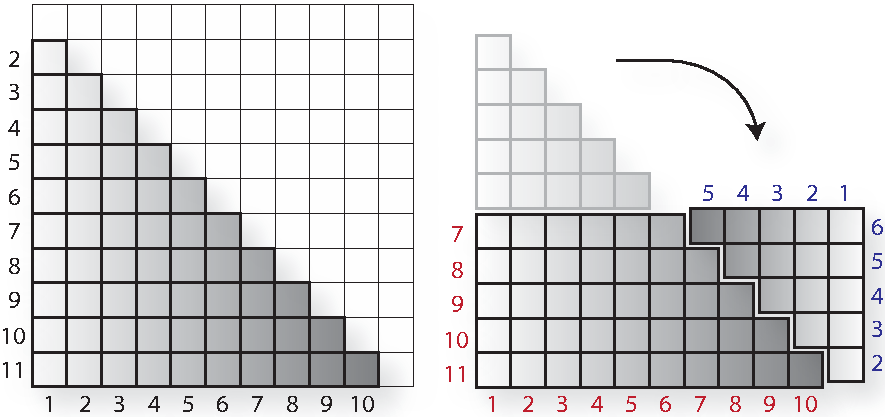
\includegraphics[width=4in]{Chapter2/tri_to_rect.pdf}
\caption[Distribution of triangular matrix work load]{Example of the recoding of the search space coordinates from a triangular to rectangular grid for efficient distribution across multi-core CPU clusters for 11 SNPs, as detailed in algorithm \ref{algo:rectangularisation}. The upper and lower triangular matrices are symmetrical, so only the shaded area is scanned (left). As the scan proceeds through the rectangular grid (right) iterating through rows $i = \{7,...,11\}$ and columns $j = \{1,...,11\}$. If $i > j$ then the SNPs tested are chosen according to the corresponding coordinates in red. If $i \leq j$ then the coordinates in blue are chosen.}
\label{fig:tri_to_rect}
\end{center}
\end{figure}


While the LPT achieves good efficiency, particularly with a very large number of available cores, it can be improved further. Here an alternative algorithm is devised that restructures the search grid to enable a computationally tractable and theoretically balanced work load across an arbitrary number of cores. First, the lower triangular matrix is partitioned into two sections by bisecting along the row $i = \lceil p / 2 \rceil$. By rotating the upper section (triangular matrix), and adjoining its diagonal with the diagonal on the lower section, a new rectangular matrix $R$ is created with dimensions $\lceil p / 2 \rceil$ rows and $p + l$ columns, where $l$ is 1 if $p$ is even, and $0$ otherwise (figure \ref{fig:tri_to_rect}).The search space is then simply distributed amongst cores by evenly partitioning the rows. Algorithm \ref{algo:rectangularisation} maps from the refactored rectangular matrix $R$ back to the coordinates of the original triangular matrix $F$, where the function
\begin{equation}
u(p, c, C) = \lceil cp/C(\lfloor p/2 \rfloor + 1) \rceil
\end{equation}
defines the row position of $R$. 

\begin{algorithm}
\caption{Rectangularisation and parallel distribution of triangular matrix}
\label{algo:rectangularisation}
\begin{algorithmic}

\IF{$c = 1$}
  \STATE $b_i := \lfloor p/2 \rfloor + 1$
  \STATE $e_i := u(p, c, C)$
\ELSIF{$c = C$}
  \STATE $b_i := u(p, c-1, C)+1$
  \STATE $e_i := p$
\ELSE
  \STATE $b_i := u(p, c-1, C)+1$
  \STATE $e_i := u(p, c, C)$
\ENDIF
\IF{$odd(p)$}
  \STATE $l := 1$
\ELSE
  \STATE $l := 0$
\ENDIF

\FOR{$i := b_i$ to $e_i$}
  \FOR{$j := 1$ to $p-l$}
    \IF{$j < i$}
      \STATE $F_{ij} := R_{ij} := f(y, x_i, x_j)$
    \ELSE
      \STATE ${i}' := p - i + 2 - l$
      \STATE ${j}' := p - j + 1 - l$
      \STATE $F_{{i}'{j}'} := R_{ij} := f(y, x_{{i}'}, x_{{j}'})$
    \ENDIF
  \ENDFOR
\ENDFOR

\end{algorithmic}
\end{algorithm}

\subsection{GPU optimisation}

The scan follows a single instruction-multiple data (SIMD) model, such that a fairly intensive kernel (the F test) is performed repeatedly on a large grid of data. The OpenCL (open source computing language) has been developed to allow multi-core architectures to generically parallelise such analyses. Of particular use is the ability of OpenCL to harness the massively multi-core architecture of modern graphics processing units (GPUs). Another such API, CUDA (compute unified device architecture), can also be used, however it is restricted to NVIDIA devices only. OpenCL was chosen for use in {\tt epiGPU} because it is open source and avoids the problem of being hardware vendor specific.

While most GPUs have hundreds of cores, performance doesn't necessarily scale proportionally, and not all algorithms will benefit from GPU parallelisation (\emph{e.g.} \citealp{Davis2011}). The main performance limiting factor is the memory input/output (I/O) bandwidth between processing cores and video memory. The computational kernel that runs on the GPU cores restructures the regression algorithm, making efficient use of the video memory hierarchies and this was necessary for achieving significant speed improvements. Several steps were necessary to limit the kernel I/O operations whilst maximising its efficiency, as outlined below.

\paragraph{Distribution strategy} The processing cores of the GPU are divided into groups of 8, known as streaming multiprocessors (SMs). These spawn and enqueue multiple threads for the execution of the kernel function, each thread being an F test for a different SNP pair. Ideally the number of threads per SM should be made as large as possible in order to minimise communications between CPU and GPU, and to reduce the number of kernel initialisations. However, for most operating systems the SM must not be occupied for more than 5 seconds (to allow other graphical devices to function), so the number of possible threads is restricted. The lower triangular $p \times p$ search grid must, therefore, be partitioned into a dense grid, such that each grid element can be sent to the GPU and executed within the allotted time.

\paragraph{Memory layout} GPUs partition their memory into four sections (in decreasing order of size, increasing order of speed): RAM, cache, local memory (L2), and private (L1). It is of primary importance to minimise time in piping data from various memory regions to the processing cores in order to achieve efficiency. The genotype data comprises the bulk of the information for performing the scan. This had to be mapped to the video random access memory (RAM), which is hierarchically the largest memory space but also the slowest to access. The phenotype is read only and, comprising a single vector of single precision floating point values, is stored in a smaller section of RAM that has faster access. Ideally this would be stored in L2 or L1 memory because it is accessed by every core for every F test, however these sections are extremely small, restricting this possibility. L2 and L1 share 16 kilobytes (kb) within each SM, effectively allowing 2kb per core. This was used to accrue the calculations for the nine genotype class means, $x_{ij}$, in $e.g.$ equation (\ref{eq:nullfull}) for each concurrent thread.

\paragraph{Use of on-line algorithms} Calculating the sum of squares of $y$ is conventionally done as
\begin{equation}
SS(y) = \sum^n (y - \bar{y})^2 \label{eq:ssy}
\end{equation}
where $n$ is the number of individuals. However, this would be problematic because of the requirement to first calculate the mean value of $y$ before being able to calculate its sum of squares. This isn't a problem when there are no missing values in the genotypes, because these values would not change, and they could be passed as precalculated values to the kernel. However, with missing values existing (as is often the case) an alternative method was devised. On-line algorithms are such that they can process the data incrementally in the order that the input is fed to them. In contrast, equation (\ref{eq:ssy}) is an off-line algorithm because it requires to have had access to all data prior to the calculation in order to calculate $\bar{y}$. This calculation was restructured to be made on-line based on \cite{Welford1962}, where $\bar{y}$ and $SS(y)$ for the entire cohort were passed to the kernel (calculated once for the whole scan on the CPU), and for every missing genotype value the individual's contribution was omitted according to Algorithm \ref{algo:on-line}, where the function $missing(X_{ik})$ tests if the $k$th individual's genotype at SNP $x_i$ is missing, and $\tilde{n}$ is the number of individuals with no missing genotypes for the pair of SNPs under test.

\begin{algorithm}
\caption{On-line algorithm for updating $SS(y)$ and $\bar{y}$}
\label{algo:on-line}
\begin{algorithmic}

\STATE $\tilde{n} := n$
\STATE $\tilde{SS(y)} := SS(y)$
\STATE $\tilde{\bar{y}} := \bar{y}$
\FOR{$k := 1$ to $n$}
\IF{$missing(X_{ik}) \cup missing(X_{jk})$}
\STATE $\tilde{SS(y)} := \tilde{SS(y)} - (y_k - \tilde{\bar{y}})(y_k - (\tilde{n}\tilde{\bar{y}} - y_k)/(\tilde{n}-1))$
\STATE $\tilde{\bar{y}} := (\tilde{n}\tilde{\bar{y}} - y_k)/(\tilde{n}-1)$
\STATE $\tilde{n} := \tilde{n} - 1$
\ENDIF
\ENDFOR

\end{algorithmic}
\end{algorithm}


\paragraph{Vectorising phenotype reads} The two major hardware vendors of graphics cards, ATI and NVIDIA, have both implemented hardware level vectorisation capabilities. Theoretically this means that 4, 8 or 16 array elements can be fetched from video RAM to L2 memory in the time that fetching a single array element would take using the non-vector form. These memory channels were used to read the phenotype values by the kernel.

\paragraph{Bit-packing genotype data} Each genotype is encoded as 0, 1, 2 to denote the number of minor alleles, or 3 to denote a missing value. Therefore only two bits are required to store a single genotype, such that even by storing them as $char$ data types, the smallest native data type in ANSI C at 8 bits, is relatively wasteful of bandwidth when the kernel fetches the data from RAM to L2. A beneficial trade-off could be made whereby encoding the genotype array to bit-pack 16 genotypes into an $int$ data type (32 bits) would increase transfer rates sufficiently even with the small cost of the kernel having to unpack the data upon its arrival for processing. For example, say the genotypes for an individual are $\{0, 1, 2, missing\}$, when encoded as normal, using an array of $char$ data types this would be stored as $\{ 00000000, 00000001, 00000010, 00000011 \}$, but the corresponding encoding when bit-packed would be a single $char$ element comprising the last two bits of each array element, $\{ 00011011 \}$. Another obvious benefit is that the genotype data requires much less space in video RAM, so even extremely large datasets could be comfortably accommodated on most GPUs.


\section{Results}

The software produced geometrically parallelises exhaustive searches for pairwise epistatic associations with quantitative traits. Large scale analyses were performed on simulated data, typical in scale of those that would be expected based on GWASs already published, on several different software and hardware systems. The performance tests show that against the baseline system (serial code running on a modern CPU) graphics cards can perform the same analysis almost two orders of magnitude faster and at minimal expense (Table~\ref{tab:parallel}), such that an analysis that would take over 4 days to complete using {\tt episcan} in serial mode could be performed in just over an hour by using software utilising a graphics card. It is demonstrable that to achieve comparable speeds using CPU cores would require a large compute cluster, for which the cost to acquire and administer could be prohibitively expensive.

Compared to existing software, these implementations appear to perform favourably. Comparing {\tt episcan} against {\tt FastEpistasis}, both running in serial, {\tt episcan} runs approximately $3.5\times$ faster, performing $128200$ tests per second. Both programmes scale almost linearly with the number of cores. {\tt EPIBLASTER} is the most efficient GPU based implementation currently available, and {\tt epiGPU} (using the values from the Nv GTX285, a similar card to the one used by \cite{Kam-Thong2010}) performs almost $4 \times$ faster in terms of tests per second.

\renewcommand{\arraystretch}{1.2}
\begin{table}[!t]
\rowcolors{3}{tableShade}{white}
\begin{threeparttable}
\caption{\label{tab:parallel}Parallelisation performance and cost comparison}
\begin{tabular}{llrrrr} \toprule 
Parallelisation & Hardware & \multicolumn{1}{c}{Cost} & \multicolumn{1}{c}{Time} & \multicolumn{1}{c}{Relative} & \multicolumn{1}{c}{Cost} \\
& & \multicolumn{1}{c}{/ \textsterling \tnote{d}} & \multicolumn{1}{c}{/ min \tnote{e}} & \multicolumn{1}{c}{Speed \tnote{f}} & \multicolumn{1}{c}{benefit \tnote{g}}\\ \toprule
None 	& Baseline CPU \tnote{a} & - & 5860 & 1.0 & -\\
%& & & & \\
%\midrule
Multi-core CPU	& 6-core CPU \tnote{b} & 760 & 986 & 5.9 & 1.6\\
		& 8-core CPU \tnote{c} & 1600 & 763 & 7.7 & 1.0\\ 
%& & & & \\
%\midrule
CPU cluster \tnote{c}	& 16-core cluster & - & 398 & 14.7 & -\\ 
		& 32-core cluster & - & 195 & 30.0 & -\\ \
		& 64-core cluster & - & 96 & 61.0 & -\\ 
%& & & & \\
%\midrule
GPU	& Nv Fermi GTX580 & 367 & 63 & 91.6 & 51.9\\
		& ATI Radeon 6970 & 300 & 86 & 68.1 & 47.2\\
		& Nv Tesla S1070 & 960 & 146 & 40.1 & 9.0\\
		& Nv GTX285 & 230 & 145 & 40.1 & 36.2\\
		& Nv 8800GT & 72 & 613 & 9.6 & 27.7\\ \bottomrule
\end{tabular}
\begin{tablenotes}{\footnotesize
\item[a] Baseline equipment, Intel i7 970 3.2GHz, running in serial
\item[b] Intel i7 970 3.2GHz
\item[c] Dual Intel Xeon E5472 3.0GHz
\item[d] Approximate cost for equipment above baseline. Cost estimates for large compute clusters are too subjective for realistic comparisons
\item[e] Total user time to complete the analysis (300,000 SNPs, 1000 individuals)
\item[f] Time relative to baseline time
\item[g] Cost benefit calculated as Speed / Cost, figures shown are adjusted relative to the cost of the best performing desktop CPU alternative (8-cores).}
\end{tablenotes}
\end{threeparttable}
\end{table}

The use of graphics cards as tools for scientific research is a rapidly emerging industry that has manifested staggering improvements in performance over the last few years. However it is still in its infancy, and as reflected in figure \ref{fig:gpuoptimisation}, the level of manual optimisation required by developers to harness this power is considerable. Furthermore, while a very heterogeneous array of devices can be used for OpenCL applications, differences in their architectures inevitably results in different responses to optimisation strategies. Figure \ref{fig:gpuoptimisation} shows that without careful optimisation, even the most recent GPUs will appear to offer little to no advantage over CPU implementations.

\begin{figure}
\begin{center}
\includegraphics[scale=0.7]{Chapter2/gpuoptimisation.pdf}
\caption[Assessment of GPU optimisation techniques]{Incremental improvements in performance by incorporating different GPU optimisation methods. For reference, the CPU speeds for {\tt episcan} are shown as horizontal lines (serial and parallelised on Dual socket Intel Xeon E5472). Speeds are for calculating 8 d.f. F tests with 1000 individuals.}
\label{fig:gpuoptimisation}
\end{center}
\end{figure}


\section{Discussion}

Quantitative genetics has long been occupied with the theoretical contribution of genetic variants to complex traits. The last decade has seen a global effort to start investigating this empirically on a large scale, yet epistasis remains largely unexplored. Computing exhaustive pairwise epistatic scans is an important step in making tractable the understanding of non-additive genetic effects in complex traits. Shown in this study, this can be achieved efficiently by using consumer level graphics cards, an established technology that is cheap and widely available. In its current implementation, {\tt epiGPU} is limited to performing linear regression on quantitative traits, but the parallel decomposition framework is sufficiently generic to allow its extension to other pairwise statistical analyses relatively easily, such as Chi-square testing for case-control data.

Another central problem with epistasis scans is the heavy multiple testing penalty incurred by stringent significance thresholds. Computationally straightforward methods such as the Bonferroni correction are likely to penalise for an overestimated number of independent tests, and this is particularly problematic with epistasis where the dimensionality of the search is increased. However, with the growing availability of GPU clusters (\citealp{Fan:2004:GCH:1048933.1049991}), it is now becoming feasible to perform two-dimensional genome-wide permutation analyses to generate more accurate estimates of family-wise false discovery rates (\citealp{Churchill1994a}), a potentially critical step toward understanding the contribution of epistasis towards complex traits.

It should also be noted that there is no consensus on how traditional brute force techniques might compare against the emerging machine learning methods, based on techniques such as random forests or support vector machines. To effectively evaluate statistical performances of these methods, computational problems must be minimised in order to perform meaningful simulations and to generate accurate family wise false discovery rates.




\chapter{Significance thresholds for exhaustive two dimensional testing}
\label{Results3}
\lhead{Chapter 4. \emph{Significance thresholds for exhaustive two dimensional testing}}

\section{Abstract}
\setstretch{1}
Genome wide association studies impose a heavy multiple testing penalty which is detrimental to their power, so the question of significance thresholds is important. In one dimensional scans this has been explored deeply, and it can be demonstrated that because of correlation between the SNPs being tested, the effective number of tests is much lower than the actual number performed. But the degree to which this is the case in two dimensional searches for epistasis has been difficult to determine because of computational obstacles. With the emergence of GPGPU clusters, such investigations are now feasible and using the {\tt epiGPU} software (described in chapter \ref{Results2}) thousands of permutations were performed to estimate empirically the effective number of tests in two dimensional scans and a function to estimate thresholds for arbitrary SNP densities and sample sizes was derived. It is shown that previous estimates of the effective number of tests have been overestimated, and that while statistical parameterisation used in the analysis has little influence on the empirical threshold for significance, population sample size and SNP density are important. Through simulation it is also shown that inflation of the type 1 error rate as a consequence of non-normality of the response variable is a function of allele frequencies, with liability increasing as the smallest class sizes of SNP pairs decrease.

\section{Introduction}
\setstretch{1.6}
The aim of this chapter is to investigate the distribution of test statistics produced by exhaustive two-dimensional searches for very large sets of parameters. Specifically, it seeks to examine the effects of different conditions on the 5\% significance level for association between pairwise epistatic loci and phenotypes of interest.


\subsection{Multiple testing and the curse of dimensionality}

The human genome is approximately 3 billion base pairs in length. This comprises around 20 thousand genes, and while in European populations each individual is likely to differ from some reference sequence at around 3 million positions \citep{Durbin2010}, there are probably over 12 million common (with $>1\%$ allele frequency) single nucleotide polymorphisms (SNPs) within populations \citep{Altshuler2010}. So in the context of genome wide association studies (GWASs), which aim to give equal weight to all genomic loci, even when the number of observed SNPs in the study are a fraction of those that might be segregating in the population there are an extremely large number of features to evaluate for association with the trait of interest. Herein lies the problem of multiple testing. In the frequentist sense, a $p$-value denotes the probability of obtaining a test statistic at least as extreme as the one obtained from the data sample, given that the model assumptions and the null hypothesis are true. Therefore when testing a large set of SNPs for departure from the null hypothesis, that the variance of the phenotype explained by the SNP is zero, extreme $p$-values will necessarily be obtained as multiple draws are taken from the underlying distribution of the test statistic. One of the challenges of the multiple testing problem is in defining a statistical threshold whereby those signals that we deem to be significant are truly associated with the phenotype at a reasonable level of certainty.

Ultimately, employing a strategy that tests for everything has been costly for power. To significantly reject the null hypothesis an association must comprise an extremely large effect, its magnitude being a function of the effective number of tests being performed. While expanding the density of a GWAS to improve genome coverage ostensibly the effect size required for significance will increase also and this is particularly problematic for highly polygenic traits. Supposing that a very large number of variants have real effects, it may be the case that it would be impossible for any of them to have a significant effect because the amount of variance that they can explain is constrained by the number of effects that exist. Such a phenomena is fairly robust to the distribution of causal effect sizes \citep{Daetwyler2008}, and the unexpectedly poor performance of GWAS has often been attributed to this hypothesised infinitesimal model of polygenicity \citep{Park2010}.

This problem is magnified in the case of epistasis. By increasing the search space to two or more dimensions, the accompanying inflation in multiple testing results in extremely stringent thresholds. This problem, the so-called `curse of dimensionality' \citep{Bellman1957}, is intrinsic to many aspects of data mining and machine learning. With multiple statistical testing the issue is clear, the exponential increase in the multiple testing with the increase in dimensionality calls for an exponential increase in the magnitude of test statistics in order to confidently reject the null hypothesis. It is entirely possible that the current mode of study of the highly polygenic architecture underlying complex traits is rendered intractable by this. Another common problem is in the relationship between testing dimensionality and sample size. For typical sample sizes in GWAS most pairwise genotype-phenotype maps will comprise sufficient individuals per genotype class to ascertain a reasonable estimate of class effect, but for lower frequency SNPs this will not be the case. With missing genotype classes in the sample estimates cannot be made, and therefore the utility of such an approach for prediction is diminished. While pairwise SNPs only comprise nine genotype classes, this problem becomes universal to all SNP frequencies as the dimensionality increases - there being 27 genotype classes for three-way maps and 81 genotype classes for four-way maps. Known as the Hughes effect \citep{Hughes1968}, the only solution is to have extremely large sample sizes and while extremely costly for some traits, for others there may not even be sufficient numbers in the population.

The stark reality is that the search for epistatic variants is truly cursed by the problem of dimensionality. Simulations show that marginal effects are often insufficient to detect epistatic variants even when the multiple testing correction is at a lower dimension (\citealt{Marchini2005}; Chapter \ref{Results1}), and with the problem of polygenicity causing even one dimensional scans to be intractable then two dimensional searches may be out of the question. Understandably, there has been extensive investigation into the question of how to suitably define significance thresholds in one dimensional GWASs, with a view to optimise the balance between false positives and false negatives. With the advances in computational methods described in Chapter \ref{Results2} it is now possible to translate these methods to two dimensional searches.

\subsection{Threshold strategies in one-dimensional studies}

Consider a dataset upon which a family of tests are performed, each of which seeking to test the same hypothesis. Given some nominal type 1 error threshold, $\alpha = 0.05$, assuming that all the tests are independent, the probability of incorrectly finding at least one of the tests from the family to be significant is $(1 -$ the probability that none of the tests in the family are significant$)$, or $\alpha_{F} = 1 - (1 - \alpha)^{t}$, where $t$ is the number of tests (or SNPs) in the family. The \v{S}id\'{a}k correction \citep{Sidak1967} rearranges this equation to deliver a significance threshold such that the family-wise error rate, $\alpha_{F}$, is equal to the initial nominal type 1 error,
\begin{equation}
\alpha_{sidak} = 1 - (1 - \alpha_{F})^{\frac{1}{t}}. \label{eq:sidak}
\end{equation}
A common approximation to this is the Bonferroni correction, which can be derived from equation \ref{eq:sidak} as the first linear term of its Taylor expansion \citep{Holm1979}, is marginally more stringent,
\begin{equation}
\alpha_{bonf} = \frac{\alpha}{t} \leq \alpha_{sidak},
\end{equation}
but much more widely used, most likely because of historically being computationally simpler. Both of these approaches are threshold measures, they design a significance level at which a reasonable family-wise error rate is permitted, such that the probability of a false positive from within a family of tests is $\alpha_{F}$. An alternative approach is to control the expected proportion of errors amongst the tests that reject the hypothesis, or to calculate the false discovery rate for the treatment of a family of tests. A popular method, the Benjamini-Hochberg correction \citep{Benjamini1995a} details a procedure whereby all $p$-values from the family of tests are sorted into ascending order $P = \{p_{1} \leq p_{i} \leq ... \leq p_{t}\}$, and the largest $i = i^*$ that satisfies
\begin{equation}
p_{i} \leq \frac{i}{t}\alpha
\end{equation}
denotes the set of $P_{1 ... i^*}$ amongst which the probability that a hypothesis is falsely rejected is $\alpha$. This approach may be particularly useful where there are expected to be a reasonably large number of true positives.

However, both adjustment styles are lower bound estimates of the true $\alpha_{F}$ when the assumption of independence between tests is violated. Although commonly used in GWAS, the correlation structure between markers in a SNP panel is strong, and so using a correction based on $t$ alone is overly stringent. This is intuitive because if two SNPs are in complete LD then in effect only one hypothesis is being performed. Similarly, if LD is incomplete but greater than $0$ then a proportion of the variance in the first SNP is being included as part of the hypothesis in the second SNP, so it can be supposed that somewhere between 1 and 2 tests are effectively being performed. Many attempts have been made to adapt multiple testing correction methods to take into consideration the correlation structure within SNP panels. They can be broadly divided into three groups - controlling the false discovery rate, calculating the effective number of tests, and calculating the underlying distribution of family-wise test statistics.

Building on the philosophy of the Benjamini-Hochberg method, the proportion of false positives (PFP) method \citep{Fernando2004} also aims to calculate what proportion of significant hits in a family of tests are false positives for some family-wise threshold $\alpha$. Theoretically it is an extension of the posterior type 1 error rate (PER) method \citep{Morton1955} which was designed to find the probability of non-linkage between a causal locus and a marker given that linkage was declared. PFP avoids explicitly correcting for multiple tests by constructing a probability of all significant hits based on the expected power of the experiment and the proportion of tests which are true negatives. Thus, provided that these parameters can be calculated (\emph{e.g.} \citealt{Mosig2001}; \citealt{Allison2002}; \citealt{Storey2001}) thresholds can be adjusted accordingly.

Alternatively, if the effective number of tests being performed in a GWAS were known, then more appropriate family-wise significance thresholds could be imposed simply by replacing $t$ with the effective number of tests in the Bonferroni or \v{S}id\'{a}k approaches, and there have been several attempts to do this. Localised permutation analysis of the HapMap data showed that on average in CEU populations approximately 150 independent tests were being performed for every 500kb region of the genome, thus suggesting a family-wise threshold of $5.5\times10^{-8}$ for the entire genome \citep{TheInternationalHapmapConsortium2005}. A less stringent threshold of $5\times10^{-7}$ was used by \citet{TheWellcomeTrustCaseControlConsortium2007}, where the posterior odds of hits being true associations were calculated to be 10:1 in favour, however such a statistical framework requires accurate estimates of power and underlying trait architectures (as with the PFP method), and these may not be easily ascertained. The threshold of $5\times10^{-7}$ was based on there being $1\times10^6$ independent regions in the genome, there being 10 underlying genes per trait, and estimated power for detection at 50\%, but assuming a highly polygenic model or a smaller sample size would elevate this threshold. Numerical approaches can also be used, for example \citet{Patterson2006} proposed a method where the effective number of tests were calculated by summing the moment estimators for the chromosomal eigenvalues. Similar methods have also been proposed \citep{Nyholt2004, Li2005, Gao2008, Moskvina2008}, however \citet{Dudbridge2008} and \citet{Salyakina2005} have shown that although these methods are useful and computationally efficient indicators of the correlation structure, generally they are not sufficiently robust to be used to derive consistent thresholds.

What is widely regarded as being the most robust method to find family-wise significance thresholds for non-independent parameters, permutation analysis, is also the most computationally intensive. Initially introduced by \citet{Fisher1935} and adapted to linkage studies by \citet{Churchill1994a}, permutation analysis seeks to sample from the tail of the distribution of test statistics for a family of tests. This is achieved by performing the genome-wide analysis $N$ times, randomly shuffling the response variable for each set of tests, and recording the most extreme $p$-value achieved each time. These are sorted into ascending order and the family-wise threshold is then set to be the $p$-value found at the $(\alpha N)^{th}$ position in the list. Critically, it has the feature of preserving the structure within the genome and the distribution of the phenotype but severing the biological link between the two, giving an empirical estimate of how extreme the test statistics are likely to go by chance alone. Although designed with the intention for use on a per-experiment basis, permutation analysis has since been invoked to attempt to uncover the effective number independent regions in the entire genome. By resampling SNPs across a continuum of densities \citet{Dudbridge2008} inferred the point at which introducing more SNPs no longer increased the permutation based thresholds to be 693138 independent regions. To be specific, this is not to say that this many SNPs will provide full coverage of the genome, rather it means that in general as SNP density increases the coverage of these regions will tend towards completion. Thus it is argued that all one-dimensional scans should use the corresponding family-wise threshold of $7.2\times10^{-8}$ because even though certain studies might use sparser panels, the intention is always to achieve genome-wide coverage, and a standardised threshold allows the comparison between different marker panels and the extension to imputed SNPs.


\subsection{Extensions to two-dimensional searches}

All of these methods invoke different philosophies and their merits can be debated. Yet it is unknown how accurately or easily they can be applied to two dimensions. The consensus approach is to simply use the conservative Bonferroni correction, but recently an attempt has been made to calculate the effective number of tests being performed in an exhaustive pairwise scan. \citet{Becker2011} used permutation analysis on Monte Carlo simulations where the family of tests are partitioned into two types: the correlation structure between interactions comprising a single SNP against an independent region of correlated SNPs (type A), and between two independent regions of correlated SNPs (type B). Using 5600 individuals genotyped at 495000 SNPs with minor allele frequencies greater than $0.05$, permutation analysis in one dimension resulted in an effective number of tests to be approximately 250000, giving a scalar correction factor of $\frac{250000}{495000} \approx 0.5$. Assuming the same correlation structure exists between type A and type B tests they initially speculated that the expected number of tests to be $0.5 \times 0.5 \times t(t-1)/2$, however it was shown that while type A correlations are identical to the correlation structures in one-dimensional tests, type B are much less correlated, leading to an estimated number of effective tests of $0.44 \times t(t-1)/2$.

Philosophically this is at odds with most of the one dimensional non-independence procedures, because it simply scales the Bonferroni correction without considering the increased correlation structure amongst SNPs as the density increases. In addition there are a few other concerns that an inference method will fail to address. One possibility is that as the search increases in dimensionality, particularly for small sample sizes the combinatorial enumeration of the partitioning of phenotype values across genotype classes reaches exhaustion. That is to say that the most extreme assortment of individuals into genotype classes will inevitably occur eventually if the number of genotype combinations is sufficiently large, such that any true biological signal will be at best only as good as the combinatorially optimum configuration. At which point this may start to happen is difficult to calculate, as it depends on several factors including the distribution of class sizes and the dimensionality of the test. Nonetheless, small class sizes amongst small sample sizes are likely to maximise the chance of this occurring.

Another important issue is the impact on the distribution of $p$-values should violations in the assumptions of the test statistic occur. Many studies have documented the problems associated with departure from parametric assumptions for parametric tests and of particular interest in exhaustive searches is the extent to which such violations will impact results under different conditions (\emph{e.g.} \cite{Boneau1960, Sawilowsky1992, Cribbie2003}). A major concern is that there may exist an inflation in the type 1 error, and this can result in two possible outcomes. Firstly, without knowledge of the behaviour of test statistics when violating parametric assumptions experiments are liable to return a higher rate of false positive results. Secondly, with correction for type 1 error inflation, for example by adjusting experiment wise significance thresholds, the power may be affected, causing an increase in type 2 errors. An interesting conundrum that may arise with high dimensional searches often occurs when significant effects are discovered where genotype classes with few observations but extreme effects explain most of the genetic variance. One might be inclined to accept the validity of such a result from an evolutionary perspective because extreme effects are expected to be rare in the population. But there may also be skepticism regarding the artificial inflation of test statistics involving small genotype class sizes. This can be problematic because for example if the most `believable' 
result from a biological perspective is the least believable from a statistical perspective then the objective of an exhaustive search comes into question. Resolution in this area is required.

With the growing availability of GPGPU clusters {\tt epiGPU} can be used to begin exploring genome wide permutation tests for two dimensional scans. This study attempts to explore empirically the `gold standard' of significance thresholds, permutation analysis, in two dimensional tests, and attempts to understand the impact of violating the assumptions of normality in such searches.

\section{Methods}

This study is divided into two parts. The first part seeks to explore the impact of using non-normalised response variables in two dimensional searches through simulation, with respect to allele frequency dependent behaviour. The second part uses GPGPU clusters to enable the calculation of permutation based false discovery thresholds under differing sample sizes and SNP densities.

\subsection{Monte Carlo simulations}

A simple Monte Carlo simulation was performed to ascertain the impact on the distribution of $p$-values for two dimensional scans as a function of the minor allele frequencies at both loci. The simulation proceeded as follows:
\begin{enumerate}
\item Two SNPs, $x_{1}$ and $x_{2} \in \{0, 1, 2\}$, are simulated in Hardy-Weinberg equilibrium with allele frequencies drawn from the set of pairwise frequency bins $f_{1} = f_{2} = \{0.05, 0.10, ..., 0.50\}$.
\item A normally distributed phenotype $y$ is simulated with $\sigma = 1$ and the mean adjusted such that $min(y) = 2$.
\item An 8 d.f. F-test is performed to calculate the $p$-value for association between the SNP pair and the phenotype.
\item The test is repeated, this time using $\log_{10} y$ as the response variable, to simulate non-normality. This generates skewness such that the third standardised moment $\approx 0.015$, a similar value to the skewness in the raw BMI values described below.
\end{enumerate}
This procedure is performed for sample sizes of $n = \{500, 1000, 2000\}$ individuals, and each simulation is repeated $10^5$ times. The resulting distribution of $p$-values from each pairwise frequency bin is summarised as the $95^{th}$ percentile most extreme test statistic.

\subsection{Permutation based thresholds of two-dimensional searches}

\subsubsection{Data} \label{bmi_data}

The data used for the empirical permutation analysis combines three cohorts from genetically isolated populations and has been previously described by \citet{Vitart2008}. Recruitments were made from the Croatian islands of Vis and Korcula (approved by the Ethical Committee of the Medical School, University of Zagreb and the Multi-Centre Research Ethics Committee for Scotland), and the Italian villages in the South Tyrol province (approved by the ethical committee of the Autonomous Province of Bolzao). All participants gave written informed consent.

Body mass index (BMI) was calculated from their height and weight measurements. Outliers from the sample (BMI $> 50kg/m^{2}$) were removed from the study and the BMI values were corrected for age and sex, and normalised using rank transformation. To correct for polygenic effects, following the method developed by \citet{Aulchenko2007}, a linear model fitting the kinship matrix as a random effect was performed, using the {\tt polygenic()} function in {\tt R/GenABEL} \citep{Aulchenko2007}. The residual values from this model were used for all subsequent analysis.

The Illumina Infinium HumanMap300v1/v2 SNP bead microarrays were used to genotype DNA samples and BeadStudio software was used for their processing. Following quality control, where the criteria for inclusion were 98\% SNP call rate, 95\% individual call rate, within population Hardy-Weinberg equilibrium confidence of $p \leq 10^{-10}$ and minor allele frequency $\geq 2\%$, there remained 2476 individuals and 283971 autosomal SNPs (polymorphic in all cohorts). The sample sizes are outlined in table \ref{tab:samplesizes}. To obtain sample sizes of 1250 and 625 individuals they were randomly sampled (without replacement) from the initial pool of 2476.

\begin{table}
  \begin{center}
%  \rowcolors{3}{tableShade}{white}
  \begin{threeparttable}
  \caption{\label{tab:samplesizes}Cohort sizes}
    \begin{tabular}{lrr}
    \toprule
Cohort & Sex \tnote{a} & Count \tnote{b} \\
\midrule
Vis & 0.43 & 1083 \\
Korcula & 0.36 & 876 \\
South Tyrol & 0.44 & 513 \\
\midrule
\emph{Total} & 0.41 & 2476 \\
\bottomrule
\end{tabular}
\begin{tablenotes}{\footnotesize
\item[a] Ratio of males to females in the sample
\item[b] Sample size after quality control}
\end{tablenotes}
\end{threeparttable}
\end{center}
\end{table}


\subsubsection{Imputation}

The chip used for the genotyping comprised 300k SNPs, and with denser genotype data being unavailable one way to assess the relationship between density and thresholds is to perform the permutation analysis on imputed genotype data. The reference data used was HapMap Phase II release 21 \citep{Frazer2007}, and the original dataset was imputed to a density of approximately $3.1$ million SNPs using {\tt MaCH} software \citep{Li2009,Li2010}. Subsequently all imputed SNPs with $r^2 < 0.30$ (as calculated by {\tt MaCH}) were excluded and the remaining SNPs were trimmed to 600k by sampling to keep chromosome proportions and minor allele frequency distributions consistent with the original 300k dataset. Similarly, to obtain the 150k dataset 150000 SNPs were sampled randomly from the original 300k dataset.


\subsection{Permutations}

The software {\tt epiGPU}, described in chapter \ref{Results2}, was used to perform the permutation analyses, applying the method developed by \citet{Churchill1994a} to two dimensional scans. Nine different conditions were considered, wherein population size and SNP density varied for each condition as summarised in table \ref{tab:perm_results}. For each condition the permutation analysis proceeded as follows.

\begin{enumerate}
\item The phenotype is randomly reordered.
\item An exhaustive two dimensional scan is performed against the reordered phenotype.
\item The most extreme pairwise interaction was recorded.
\item Repeat from step 1 until 1000 different permutations are performed.
\end{enumerate}

The 100 top hits from each scan typically represent a very small proportion of all tests performed (\emph{e.g.} $100 / (300000^2 / 2) = 2.2 \times 10^{-9}$), and these are used to evaluate the allele frequency distribution of the interactions that comprise the tail of the test statistic distribution. 

To generate a threshold accounting for the effective number of tests being performed in the scan, the lowest $p$-value for each permutation is listed in ascending order and the 50$^{th}$ ($5^{th}$ percentile) value becomes the threshold estimate.

Permutations were performed for two different statistical tests, parameterising for full genetic effects (8 d.f.) or interaction terms only (4 d.f.). These are described in detail in chapter \ref{Results2}. While 8 d.f. tests can be applied for any range of allele frequencies, the 4 d.f. test is restricted to SNP pairs where there are individuals representing all 9 pairwise genotype classes because the algorithm depends on estimates of all homozygote classes to accurately calculate the marginal effects of the pairwise interaction.


\subsection{Compute resources}

Performing multiple exhaustive searches on dense SNP sets with large sample sizes was a significant computational undertaking. Two GPGPU clusters were used for the majority of the analysis: {\tt cseht} at Daresbury Laboratory, comprising thirty-two NVIDIA S1070 cards; and {\tt eddie}, provided by the Edinburgh Compute and Data Facility (ECDF), comprising eight NVIDIA S2080 cards. The average time taken for each of the tests for the different cards is shown in table \ref{tab:perm_results}. For the scans with the highest SNP density, although a reasonable number of permutations are performed, there are fewer than might be desired simply due to time constraints.


\section{Results}

\subsection{The impact of non-normalised phenotypes on false discovery rates}

Many studies have documented the problems associated with departure from parametric assumptions for parametric tests and of particular interest in exhaustive searches is the extent to which such violations will impact results under different conditions (\emph{e.g.} \cite{Boneau1960, Sawilowsky1992, Cribbie2003}). A major concern is that there may exist an inflation in the type 1 error, and this can result in two possible outcomes. Firstly, without knowledge of the behaviour of test statistics when violating parametric assumptions experiments are liable to return a higher rate of false positive results. Secondly, with correction for type 1 error inflation, for example by adjusting experiment wise significance thresholds, the power may be affected, causing an increase in type 2 errors.

A recurring problem in biology is that phenotype distributions are seldom exactly normal, most commonly due to skewness. Figure \ref{fig:mc_af} shows the results from Monte Carlo simulations that were performed to acquire the distribution of test statistics for two dimensional tests both in accordance and in violation of the assumption of normality. Here it is evident that the tail of the distribution of test statistics is more extreme as allele frequencies become rare when outliers in the distribution are introduced through skewness, but that under normality there is no such inflation of the type 1 error. Further exploration of this trend demonstrates that type 1 error inflation occurs more specifically when there are genotype classes with few samples while regressing against a non-normal phenotype (figure \ref{fig:mc_classsize}). The results indicate that when there are at least 40 observations in the smallest genotype class size then the test statistic inflation due to this level of deviation from normality is eliminated. However, the required minimum class size is likely to be a function of the skewness of the data.

\begin{figure}
\begin{center}
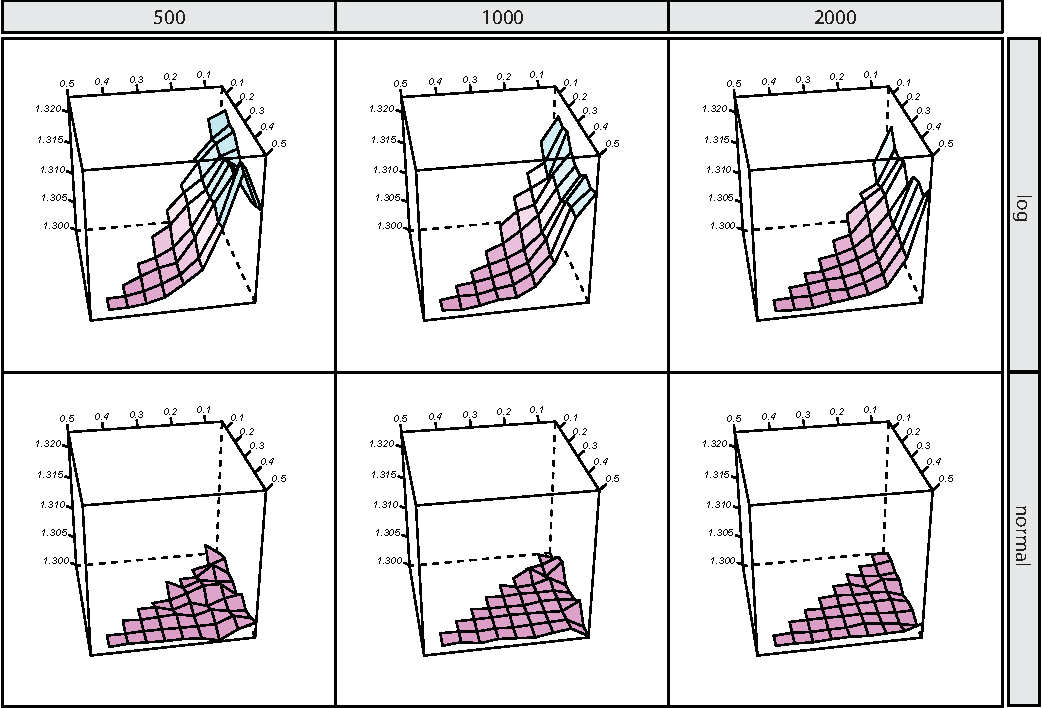
\includegraphics[width=5in]{Chapter3/fdr_5pc_wireframe.pdf}
\caption[Violation of assumptions of normality]{Results from Monte Carlo simulations showing the effect of allele frequency ($x$- and $y$-axes) on the inflation of test statistics ($z$-axis) when assumptions of normality are violated. The values of the wireframe plot are the $5^{th}$ percentile of the most extreme $-\log_{10}p$ values from $10^{5}$ pairwise tests with null models simulated at two loci with frequencies corresponding to the $x$- and $y$-axes. The top row of boxes shows the effect of using a log-normally distributed phenotype, and the bottom row when using a normally distributed phenotype. Columns of boxes represent different sample sizes.}
\label{fig:mc_af}
\end{center}
\end{figure}

\begin{figure}
\begin{center}
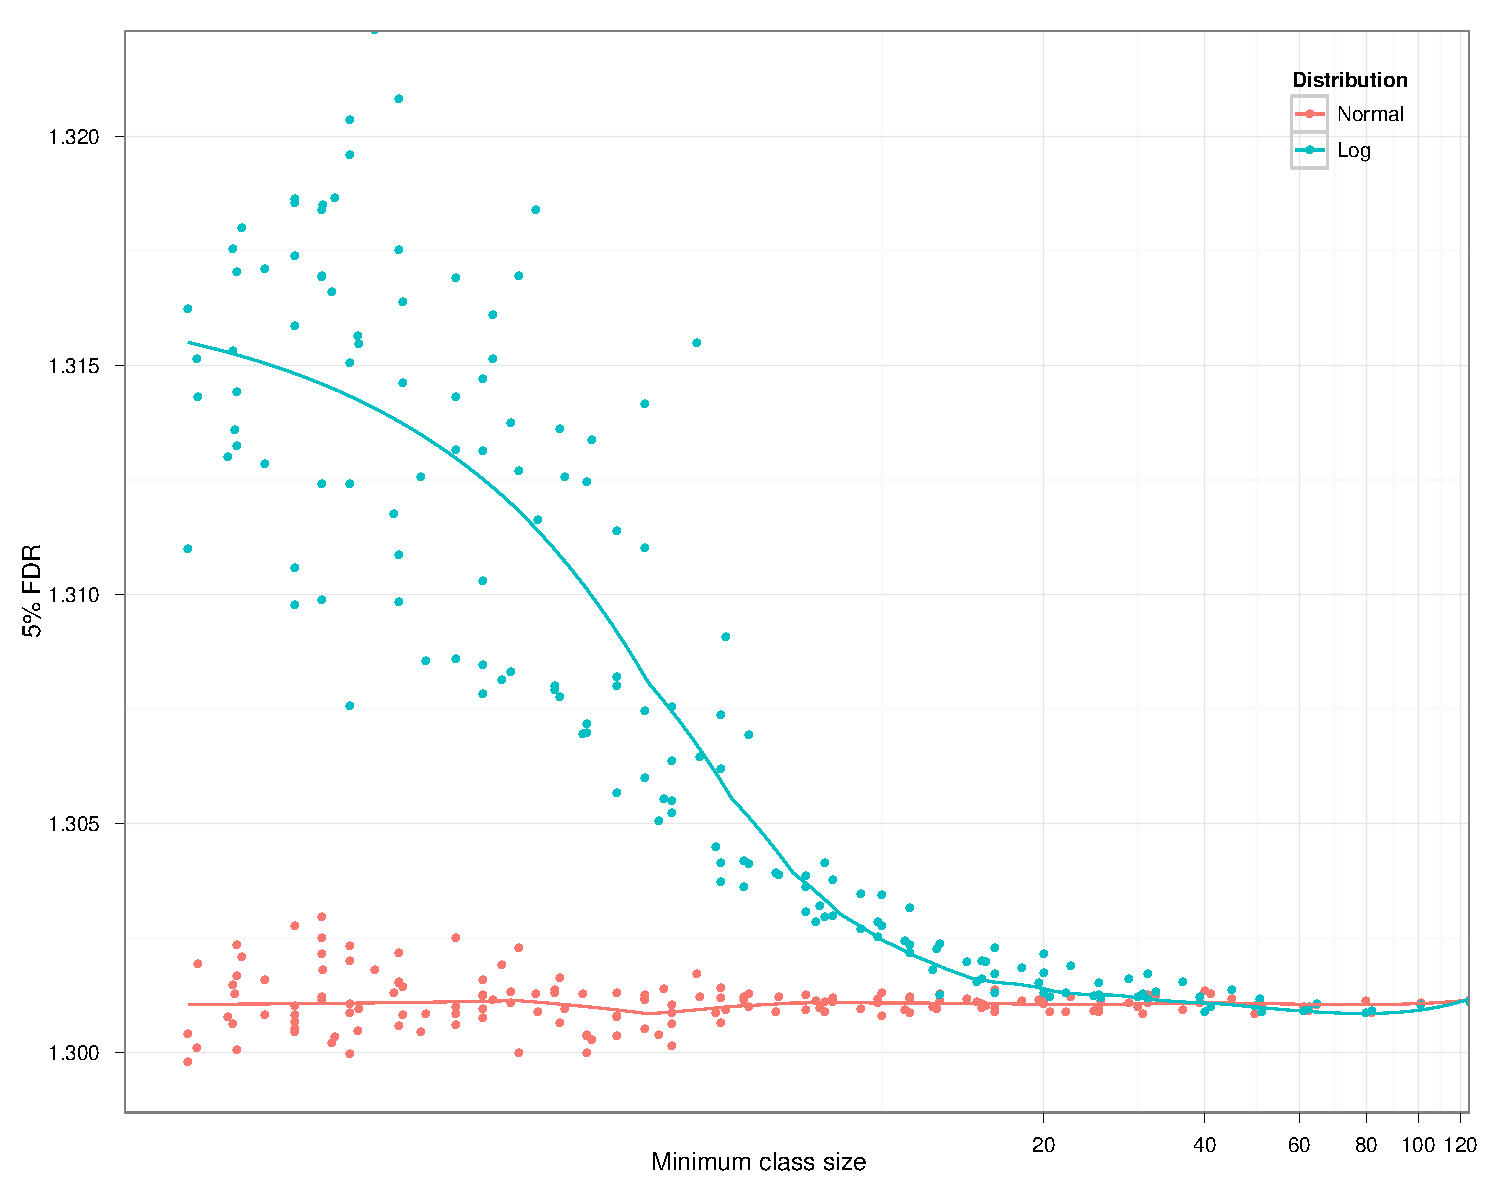
\includegraphics[width=5in]{Chapter3/inflation_vs_n.pdf}
\caption[Effect of minor class size on inflation]{The effect of the minimum non-zero genotype class size ($x$-axis, log scale) on the inflation of the test statistic for 8 d.f. epistatic tests. Data is taken from figure \ref{fig:mc_af}, demonstrating a clear trend between small class sizes and inflated test statistics for non-normal phenotypes.}
\label{fig:mc_classsize}
\end{center}
\end{figure}


The original dataset used for the permutation analysis (described in section \ref{bmi_data}) has been extensively analysed for genetic variation in BMI (Wei \emph{et al.} 2011, in preparation), and the results from these simulations may be important in their interpretation. Raw BMI values are generally skewed, resembling the log transformed distributions that were used as an example for the violation of normality in figure \ref{fig:mc_af}, and in general the most robust method to correct for non-normality is to use the method of rank transformation. Table \ref{tab:bmi_results} demonstrates the liability for false positives to occur when normality is violated in this manner. Most notably, many pairwise interactions were mined with $- \log_{10}p$-values sufficiently extreme to surpass the stringent Bonferroni correction of $11.95$. However, upon reanalysis following rank transformation of the phenotype these test statistics are significantly diminished. While few observations in certain genotype classes result in inflation, as in this case, it is important to note that under conditions of normality there is no such liability.

\begin{table}
  \begin{center}
  \rowcolors{3}{tableShade}{white}
  \begin{threeparttable}
  \caption{\label{tab:bmi_results}False positives from epistatic searches in BMI}
    \begin{tabular}{rrrrr}
    \toprule
SNP 1 & SNP 2 & MGC \tnote{a} & Raw $p$-value ($-\log_{10}$) \tnote{b} & Corrected $p$-value ($-\log_{10}$) \tnote{c} \\
\midrule
rs10789450 & rs1857985 & 6 & 13.82 & 9.87 \\
rs1217394 & rs826911 & 7 & 12.47 & 8.59 \\
rs9809255 & rs1857985 & 3 & 12.23 & 7.79 \\
rs10758713 & rs1857985 & 3 & 12.06 & 8.74 \\
rs1857985 & rs7342676 & 3 & 12.60 & 8.56 \\
rs1857985 & rs12927233 & 6 & 12.74 & 9.60 \\
rs755647 & rs2267271 & 4 & 12.61 & 8.08 \\
\bottomrule
\end{tabular}
\begin{tablenotes}{\footnotesize
\item[a] Minimum genotype class size (non-zero)
\item[b] Returned from scan using non-normalised phenotype
\item[c] Returned from scan using rank transformed phenotype}
\end{tablenotes}
\end{threeparttable}
\end{center}
\end{table}


\subsection{Permutation analyses}

Currently, there are very few exhaustive searches for epistasis being performed, and when they are being used they typically employ very conservative significance thresholds, such as the Bonferroni correction. Some efforts have been made to adjust this based on the estimated number of effective tests being performed \citep{Becker2011}, but in reality the behaviour of the extreme tail of the distribution when a very high number of multiple tests is being performed is unknown, nor is the true genomic correlation structure amongst these tests. Here, permutation analysis was used as the most direct way for answering these questions. 

The results from the permutation analysis are shown in figures \ref{fig:perm_density} and \ref{fig:thresh_error}, and table \ref{tab:perm_results}. There are several important conclusions that can be drawn from this analysis. Most importantly, the Bonferroni correction is shown to be overly conservative, and that using a scalar correction factor as in \citet{Becker2011} does not fully account for the asymptotic behaviour of the effective number of tests as SNP density increases (as shown in \citet{Dudbridge2008}).

\begin{figure}
\begin{center}
\includegraphics[width=5in]{Chapter3/thresh_error.pdf}
\caption[Empirical estimates of 2D search thresholds]{As depicted in figure \ref{fig:perm_density}, the 5\% family-wise FDR based threshold can be calculated from the distribution of maximum values from permutations (central dots). Through bootstrap analysis (10,000 resamples per permutation set) two-tailed 5\% confidence intervals were obtained for each threshold estimate.}
\label{fig:thresh_error}
\end{center}
\end{figure}

\begin{sidewaysfigure}
\begin{center}
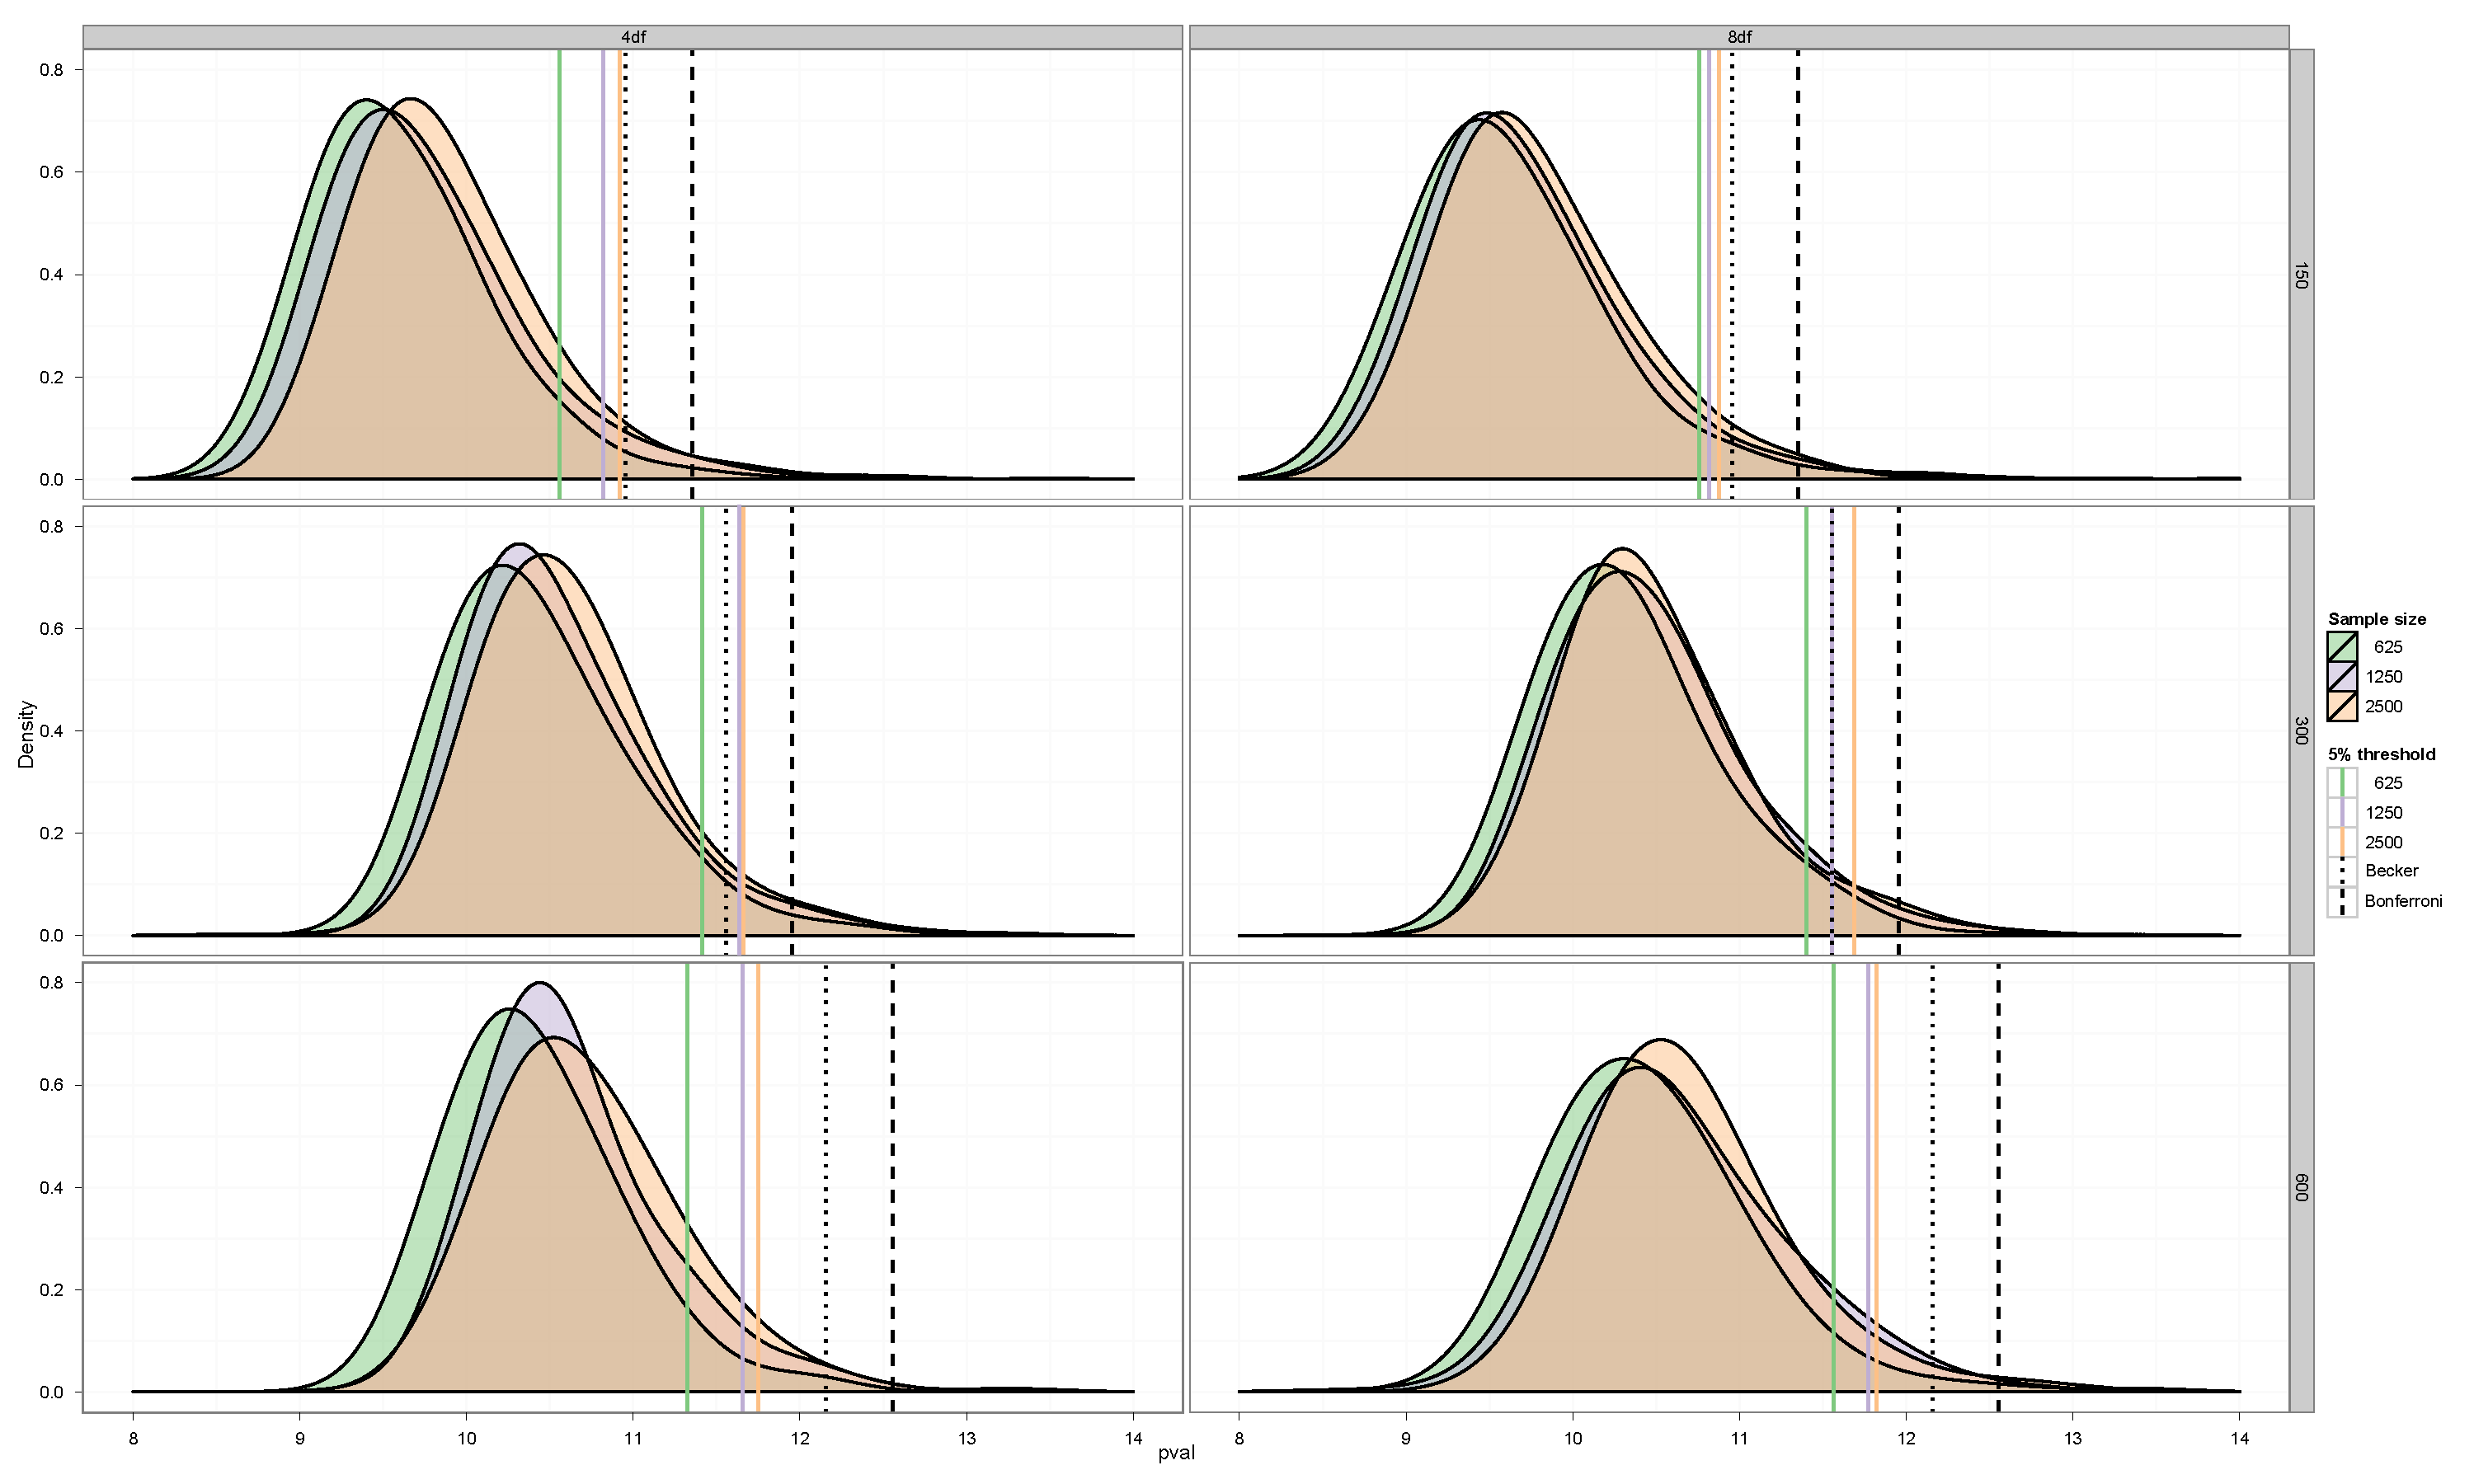
\includegraphics[width=8in]{Chapter3/perm_density.pdf}
\caption[Distribution of test statistics from permutation analysis]{Hundreds of permutations (table \ref{tab:perm_results}) were performed for two dimensional scans under varying testing conditions of SNP chip density (rows of boxes), sample size (distribution fill colour), and test parameterisation (columns of boxes). Each curve is a smoothed density of the top test statistics retrieved from each permutation representing its testing conditions. Vertical lines represent $5\%$ family-wise false discovery thresholds calculated for different sample sizes (colours), or for the extant methods of the Becker correction (dots) \citep{Becker2011} or Bonferroni correction (dashes).}
\label{fig:perm_density}
\end{center}
\end{sidewaysfigure}

\begin{sidewaystable}
  \begin{center}
%  \rowcolors{3}{tableShade}{white}
  \begin{threeparttable}
  \caption{\label{tab:perm_results}Summary of permutation results}
    \begin{tabular}{rrrrrrrrrrr}
    \toprule
Density & Sample size & Permutations & Tesla S1070 \tnote{a} & Tesla S2080 \tnote{a} & \multicolumn{4}{c}{5\% threshold} & \multicolumn{2}{c}{Effective SNPs \tnote{c}}  \\
& & & & & Bonferroni & Becker & 4 d.f. \tnote{b} & 8 d.f. \tnote{b} & 4 d.f. & 8 d.f. \\
\midrule
\multirow{3}{*}{150000} & 2476 & 1000 & 1:48 & 0:45 & \multirow{3}{*}{11.35} & \multirow{3}{*}{10.95} & 11.10 & 11.07 & 112762 & 109441 \\
& 1250 & 1000 & 0:56 & 0:22 & & & 11.05 & 11.10 & 105947 & 112472 \\
& 625 & 1000 & 0:28 & 0:11 & & & 10.97 & 10.90 & 96596 & 89496 \\
\midrule
 \multirow{3}{*}{283971} & 2476 & 1000 & 6:05 & 2:43 &  \multirow{3}{*}{11.95} &  \multirow{3}{*}{11.56} & 11.66 & 11.69 & 213480 & 221229 \\
& 1250 & 1000 & 3:08 & 1:20 & & & 11.65 & 11.55 & 212468 & 188973 \\
& 625 & 1000 & 1:35 & 0:39 & & & 11.41 & 11.40 & 160929 & 159168 \\
\midrule
 \multirow{3}{*}{600000} & 2476 & 500 & 29:42 & 11:57 & \multirow{3}{*}{12.56} & \multirow{3}{*}{12.16} & 11.77 & 11.79 & 243439 & 249695 \\
& 1250 & 500 & 15:10 & 6:04 & & & 11.67 & 11.77 & 216002 & 241078 \\
& 625 & 500 & 7:45 & 3:12 & & & 11.33 & 11.55 & 145732 & 189233 \\
\bottomrule
\end{tabular}
\begin{tablenotes}{\footnotesize
\item[a] Timings shown as \emph{hours}:\emph{minutes} per permutation as performed by {\tt epiGPU} using different hardware.
\item[b] Empirical thresholds for 5\% family-wise false discovery rates calculated from permutation results.
\item[c] Effective number of SNPs being tested based on empirical thresholds from permutation analysis.
}\end{tablenotes}
\end{threeparttable}
\end{center}
\end{sidewaystable}

Secondly, there is no significant inflation of low frequency SNPs among the permuted searches. Figure \ref{fig:mafdens} shows that the distribution of allele frequencies comprising the top 100 SNP pair hits from each permuted scan is similar to the distribution of all SNPs in the SNP panels. This is an important result, because it allows researchers to have equal confidence in hits comprising SNPs with rare frequencies as with those with intermediate frequencies, at least from the perspective of there being no artificial statistical inflation.

\begin{figure}
\begin{center}
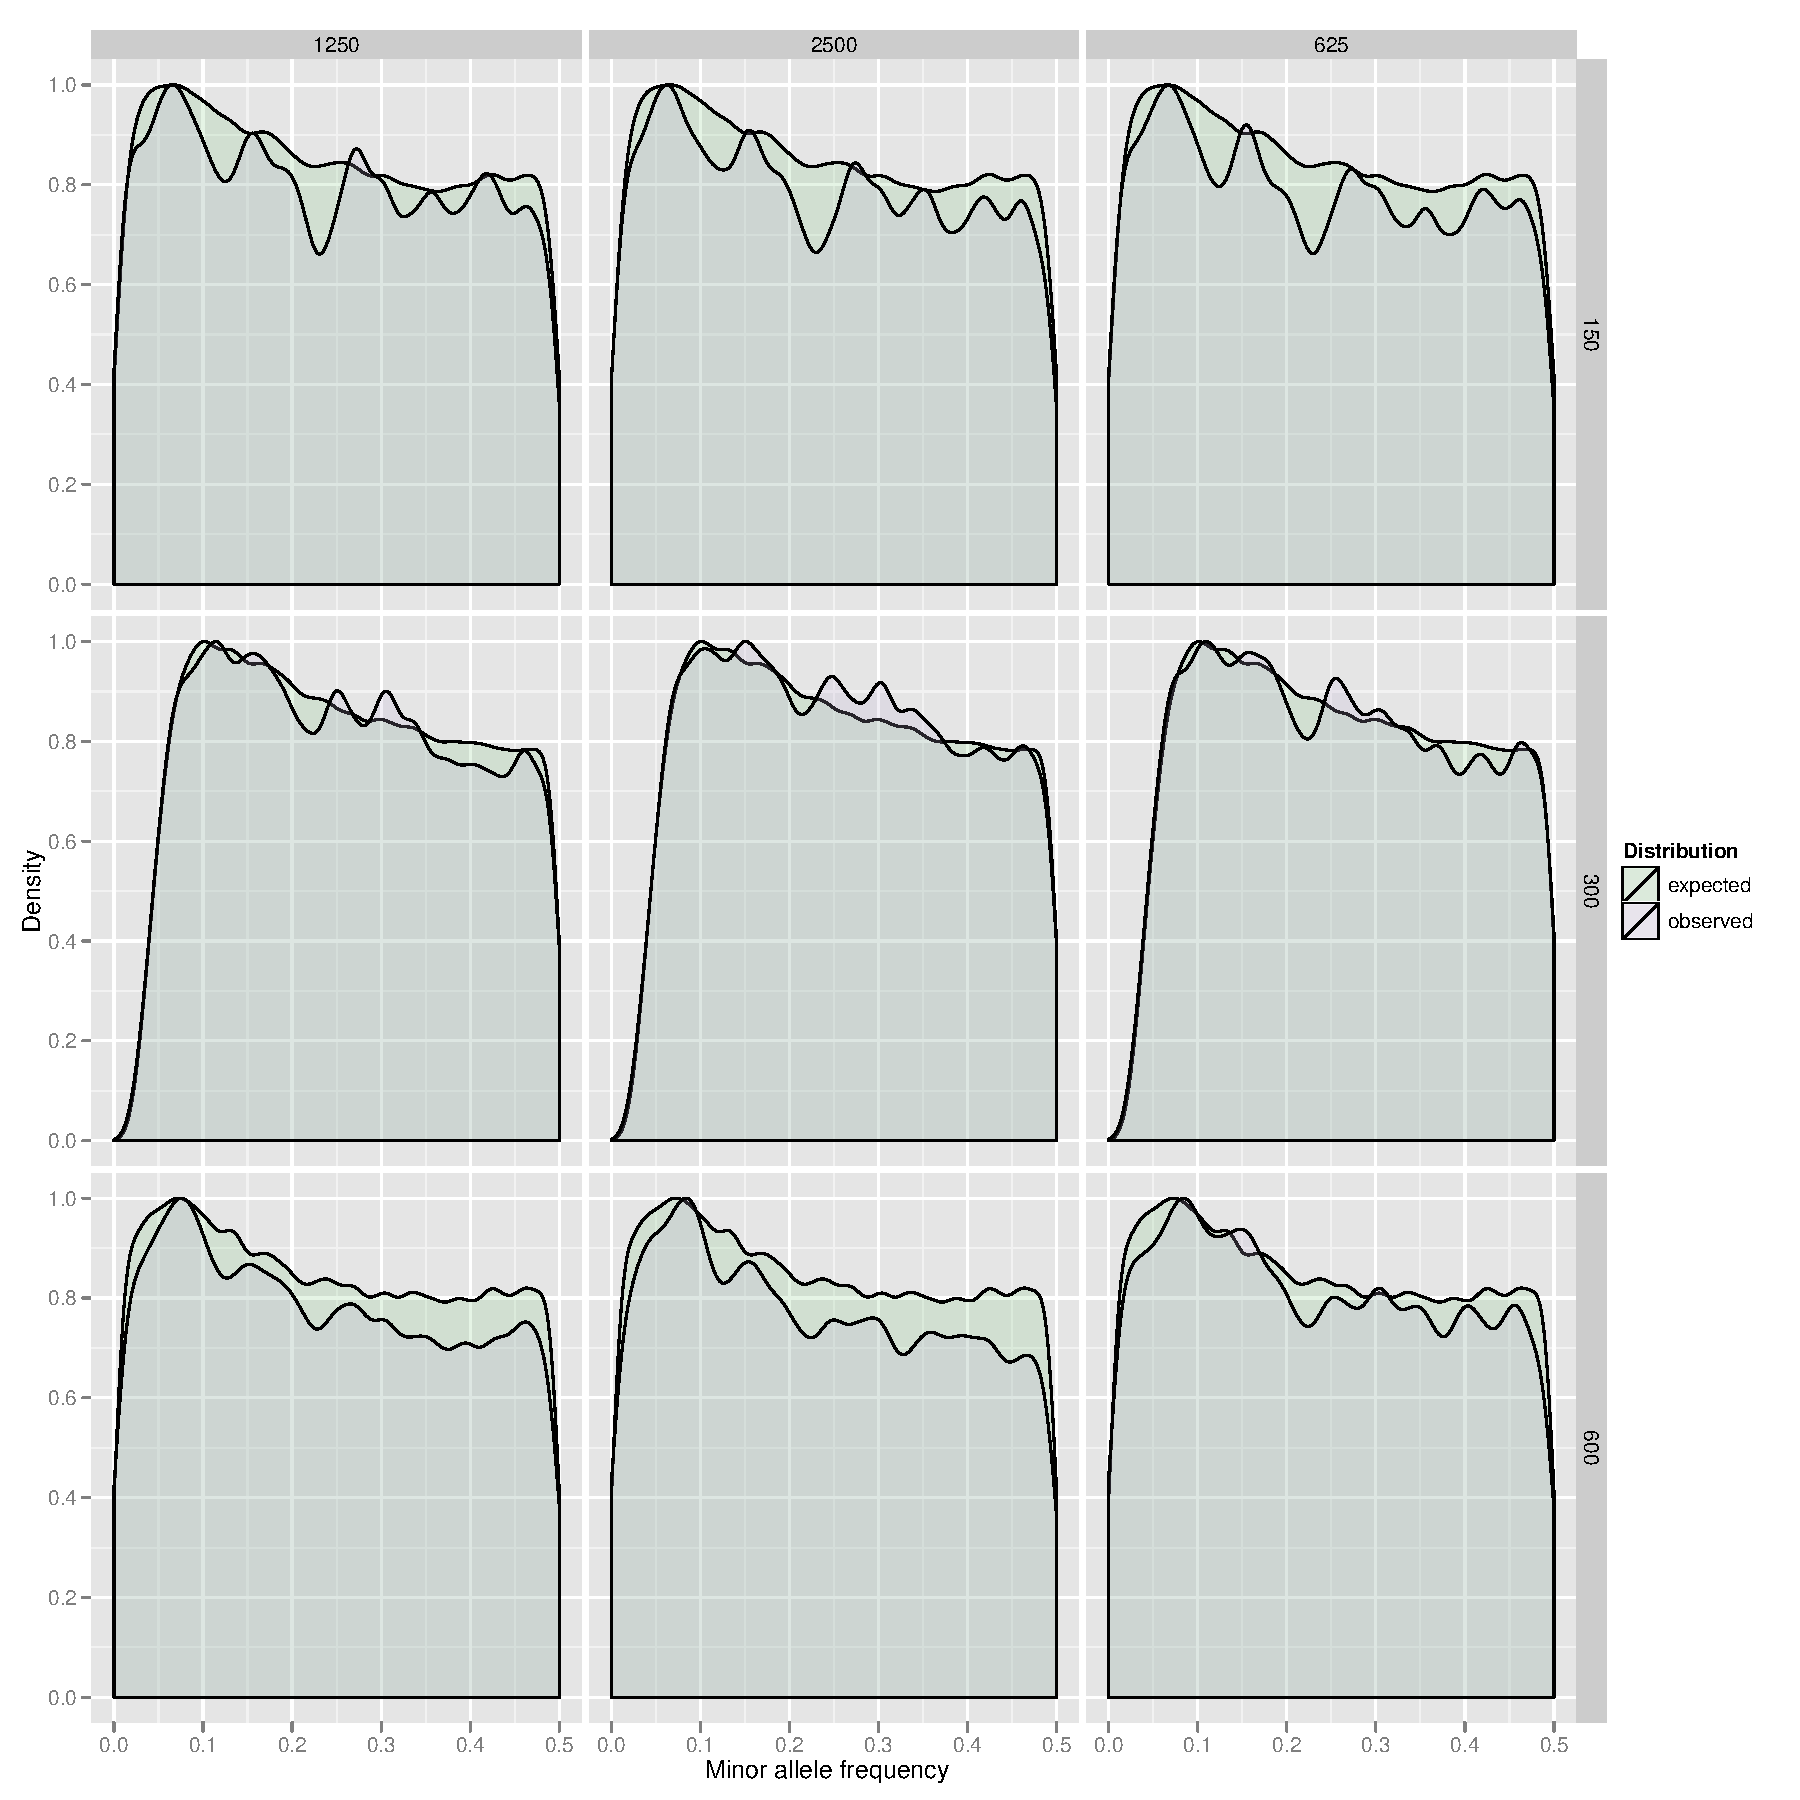
\includegraphics[width=5in]{Chapter3/mafdens.pdf}
\caption[Observed vs expected SNP frequency densities]{The frequency density of the SNP chip (red) is plotted along with the density of frequencies of the 100 most significant SNPs obtained from each permutation for 8 d.f. tests. Columns of boxes represent sample size, and rows represent SNP density ($\times 1000$).}
\label{fig:mafdens}
\end{center}
\end{figure}

Thirdly, in most cases there is no discernible impact of the test parameterisations on the thresholds. When the sample size is smallest there is a slight decrease in the estimated threshold for 4 d.f. tests. This is expected because the actual number of tests performed is expected to drop because SNP pairs that do not have observations for all 9 genotype classes are omitted from the scan for 4 d.f. tests, but not for 8 d.f. tests.

Finally, increasing sample size has an increasing effect on the threshold. While the data is insufficient to make a strong statement about this, there is a tendency for the elevation of the threshold from 625 to 1250 observations to be larger than from 1250 to 2476, and this may indicate an asymptotic relationship (figure \ref{fig:thresh_error}). To speculate on the reason for this relationship is difficult, but the following observations can be made regarding the three variables involved in the test statistic: the actual sample size $n$, the average variance explained by all tests in the scan $SS_{W} / (SS_{W}+SS_{B})$, and the average number of parameters per test $g$ (this will vary when small sample sizes have more missing genotype classes). In a background of two factors remaining fixed, the \emph{approximate} behaviours of the third factors can be described as:

\begin{eqnarray}
-\log \left ( f \left (
\frac{
 SS_{W}  (g - 1)^{-1}
}
{  SS_{B} (n - g)^{-1}
}; g - 1, n - g
\right ) \right )
& \propto &
 n \\
& \propto &
SS_{W} / (SS_{W} + SS_{B}) \\
& \propto &
-\log(g)
\label{eq:ftest_n}
\end{eqnarray}
where $f(x; d_{1}, d_{2})$ is the probability density function for some random $F$-distributed variable $x$ with numerator and denominator degrees of freedom $d_{1}$ and $d_{2}$ respectively. First of all smaller values of $n$ require more extreme data in order to achieve the same level of significance as those from larger sample sizes, however the actual distribution of $SS_{W} / (SS_{W} + SS_{B})$ from an exhaustive scan with respect to sample size is unknown, although one could intuitively suggest an inverse correlation. Secondly, the relationship between sample size and the number of parameters will follow an asymptotic function 
\begin{equation}
\lim_{n \to \infty} \bar{g} = 9
\end{equation}
so as sample size increases, the increase in $\bar{g}$ will oppose the propensity to achieve extreme $p$-values due to increased sample size. The relationship is complex and without knowing the underlying distribution for each variable it is difficult to deterministically support the empirical observation of the effect of sample size on the threshold. For the purposes of the following analysis it is assumed that it is indeed a product of some asymptotic function, although further analysis will be required to confirm this.

Although the relaxation of significance thresholds when calculated from permutation is fairly modest in these examples, the conclusion may have a further reaching utility. For each of the 18 permutation sets (3 sample sizes $\times$ 3 SNP densities $\times$ 2 test parameterisations; table \ref{tab:perm_results}) bootstrap analysis was performed to ascertain confidence intervals for the 5\% family-wise FDR (figure \ref{fig:thresh_error}). Naturally, the number of permutations performed here are constrained by computational resources, and so the results provide an approximation to the effective number of tests that will become more robust with more permutations. Nevertheless, it may be useful to attempt to derive an empirical relationship between the threshold, SNP density, and sample size. Assuming that the effect on the threshold from SNP density and sample size are independent of one another, and that they each follow an exponential asymptotic relationship toward some theoretical maximum number of tests given infinite SNP density, non-linear least squares (NLS) were performed to ascertain the parameters to the model, using the data from the $10000$ bootstrap samples for each of the 18 permutation sets.

The limit to the asymptote (the maximum number of tests with infinite SNP density and sample size) was estimated theoretically (rather than as a parameter in the NLS calculation). From the result in \citet{Dudbridge2008} the effective number of independent regions in a one dimensional GWAS is estimated to be $693138$, therefore the effective number of independent tests in a two dimensional GWAS at infinite SNP density is $\frac{693138 \times 693137} {2} = 2.4 \times 10^{11}$, giving a theoretical maximum $-\log_{10} p$-value of $12.68$. From this, for $n$ sample size and $M$ SNPs in the array the family-wise threshold $p_{T}$ was modelled as 

\begin{equation}
-\log_{10}(p_{T}) = a - a \left ( 
 s_{1} \exp \left ( 
  \frac {\ln(n) } { s_{2} } \right )
 + s_{3} \exp \left (
  \frac{ \ln(M)} {s_{4}} \right ) 
\right )^{-1}
\label{eqn:general_threshold}
\end{equation}
where the asymptotic limit was set to $a = 12.68$, and the following parameter estimates from NLS were obtained:
\begin{eqnarray}
s_{1} & = & 0.0258 \nonumber \\
s_{2} & = & 1.72 \nonumber \\
s_{3} & = & 0.0379 \nonumber \\
s_{4} & = & 2.33. \nonumber
\end{eqnarray}
This relationship is depicted in figure \ref{fig:threshold_function}.

\begin{figure}
\begin{center}
\includegraphics[width=5in]{Chapter3/threshold_function.pdf}
\caption[Estimation of 2D thresholds in the general case]{The wireframe maps the empirically derived relationship obtained in equation \ref{eqn:general_threshold}. The $z$-axis represents the estimated threshold for some given combination of sample size ($x$-axis) and SNP density ($y$-axis), and tending towards an asymptotic limit of $12.68$.}
\label{fig:threshold_function}
\end{center}
\end{figure}

% why is becker wrong?

\section{Discussion}

The question of where to set significance thresholds for whole genome searches is a long standing problem, and while the solutions are still perhaps incomplete in the one dimensional case, very little attention has been directed specifically to the context of epistasis. This chapter assesses the impact of non-normality on the inflation of type 1 errors in epistatic scans, presents the results from permutation analyses on exhaustive two dimensional searches, and attempts to derive significance thresholds that accurately reflect the effective number of tests being performed.

The first main conclusion is that it is imperative that a normal phenotype is used in order to be confident of avoiding type 1 error inflation. Specifically, the simulations here were concerned with the impact of outliers on the distribution of test statistics mainly because this was representative in the case of searches for epistatic variants contributing to the BMI variance in populations (Wei \emph{et al.} 2011, in preparation). It was shown that SNP pairs with low genotype counts were susceptible to type 1 error inflation, but such was not the case when the distribution of the phenotype was normalised using rank transformation.

In terms of the permutation analysis, the broad conclusion that can be based on these results is that the correlation structure between SNPs, as well as between pairwise tests, is relatively high, with the most extreme case showing a reduction in the threshold from the Bonferroni by almost an order of magnitude. However, although the Bonferroni approach is most conservative, the magnitude of multiple testing as estimated through permutation is still extremely high. It is perhaps not until the SNP array becomes very dense (\emph{e.g.} $>300000$ SNPs), and permutation thresholds become constrained by the asymptote (figure \ref{fig:threshold_function} and equation \ref{eqn:general_threshold}), that the use of permutation thresholds will constitute a significant advantage in power as the Bonferroni thresholds will continue to grow quadratically. Indeed, at lower SNP densities the approximate thresholds derived by \citet{Becker2011} that simply scale the number of multiple tests linearly (by 0.44) are reasonably accurate. Incidentally, the permutation results that most closely matched the Becker threshold came from the 300000 SNP density, however the Becker threshold was based on a 500000 SNP array. It could be argued that the method of performing Monte Carlo draws on relatively small sections of the genome resulted in an underestimate of the long range correlation structures, where although each long range SNP pair will be lowly correlated, there is an extremely large volume of these pairs in total.

Performing the permutations, even with the availability of GPU compute clusters, was extremely computationally demanding, and most researchers will not have access to this type of hardware. Furthermore, even with such hardware, as the SNP density increases the computational time required becomes unmanageable, and ostensibly at the higher densities the permutation based thresholds are of most utility. By using the general function (equation \ref{eqn:general_threshold}) to estimate significance thresholds for larger sized studies, it should be possible to impose a meaningful statistical threshold that takes into consideration the effective number of tests being performed in the scan as well as the impact of sample size. However there are some potential issues with using an empirically derived function. First, there are significant differences in LD structure between species, SNP manufacturers (\emph{e.g.} Affymetrix and Illumina \citep{Gao2010, Becker2011}, tagging or non-tagging SNPs \citep{Stram2004, Halperin2005}), and human ethnicities \citep{TheInternationalHapmapConsortium2005}. Second, imputation was used for the acquisition of the 600000 SNP array, and one potential issue that might arise from this is that the imputation algorithm may not capture local recombination events or population specific polymorphisms, and therefore cause an overestimation of the between-SNP correlation structure. Although the estimate of the asymptotic limit is unlikely to increase, the overestimation of correlation will result in a gentler growth toward the limit, and systematically underestimate thresholds for all densities above $\sim$ 300000 SNPs. While the latter problem can be resolved simply by using more data points and using only directly genotyped data rather than imputed data, the former problem is less easily amenable. Perhaps the most direct method would be through extensive permutation analyses under the varying conditions. Finally, the threshold estimates from the permutations are unlikely to be particularly accurate because they are based on only 1000 (or 500) randomisations. Desirable would have been to increase these numbers by an order of magnitude, and then perhaps the assumed asymptotic relationships within sample size (should they be real) and SNP densities would become more robust.

A third potential issue is that the estimate of the asymptotic limit $a=12.68$ may be overly stringent, because as alluded to in \citet{Becker2011} the effective number of tests being performed in a two dimensional scan depends on two principles - the number of independent regions, and the correlation between tests that involve one SNP, $i$, against $M$ other SNPs. The estimate of $a$ accounts for the first principle, but it does not consider the second. Intuitively this may be quite significant, because for example the marginal effect of SNP $i$ will be tested $M$ times. Although the correction factor for this was estimated to be fairly close to $1$ (\emph{i.e.} relatively insignificant correlations), a more formal investigation into this could be made. For example, a Monte Carlo based simulation that compared the Bonferroni threshold against a permutation based threshold using a panel of completely uncorrelated SNPs should find no difference if this latter type of correlation is low.

From a different perspective, one concern with high dimensional testing is that of exhausting the possible combinations of genotype-phenotype maps. For example, in the example of canalisation, where there are ostensibly two groups of individuals - those homozygous mutant at both loci (\emph{e.g.} high phenotype), and those who are not (low phenotype) - in a sample size of $n = 100$ where $r = 10$ are the double homozygotes the possible number of combinations is $C_{(100,10)} = 1.73 \times 10^{13}$, where
\begin{equation}
C_{(n,r)} = \frac{n!}{r!(n-r)!}.
\end{equation}
so given sufficient effective number of tests, the most extreme assortment of phenotypes into high and low groups will inevitably occur, such that no true biological interaction of the same map could possibly be more statistically extreme. Counteracting this is straightforward, as sample size increases the number of combinations expands rapidly, for example $C_{(1000,10)}  = 2.63 \times 10^{23}$, but this may remain a problem for very high dimensional searches (\emph{e.g.} with four way interactions, $500000^4 = 6.25 \times 10^{22}$), and several approaches that do attempt to explore higher order interactions, albeit not exhaustively, may be liable to such an issue. Relatedly, to partition the phenotypes according in the most extreme manner, such that the highest values are in one group and the lowest in another group, there is only one unordered arrangement where this could occur. But the number of arrangements with only a certain proportion of the more extreme phenotypes being assorted, rather than the exact set of the most extreme, into a single group will be large, so the combinatorial eventuality of `good' evidence for interaction may still be present. If such a process were at work, it would be most visible in the situation with the densest SNPs and the smallest sample size where one would expect to see many extreme results elevating the threshold, however there is clear evidence that the permutation threshold is actually reduced when sample size is reduced, suggesting that the search is not becoming saturated in combinatoric terms. The estimation of threshold values based on sample size has been discussed previously \citep{TheWellcomeTrustCaseControlConsortium2007}, where the logic has been that as sample size decreases then power decreases, so evidence for association should be more conservative. The results from these permutations suggest otherwise, that as sample size decreases the most extreme $p$-values that occur by chance are smaller. Further work is required to ascertain the underlying cause for this.

Anecdotally, the most extreme result from all permutations gave a $p$-value of $3.9 \times 10^{-16}$, and many were an order of magnitude more extreme than even the Bonferroni correction. It should be noted that family-wise thresholds only promise that from a set of multiple comparisons the chance of finding exactly one more extreme result is some value of $\alpha$, and they do not inform the distribution of $p$-values that comprise the $\alpha$ false discoveries. Therefore, in this context further calculation is required in order to believe a particularly extreme result with any greater level of confidence than the nominal $\alpha$ value. 

To summarise, the computations performed here demonstrate that Bonferroni corrections are overly conservative, and the \citet{Becker2011} approximation is only valid at low SNP density. Yet, the presumably more accurate empirical distributions of test statistics from exhaustive pairwise scans are still very stringent. Although their use will improve power to some extent over existing practices, particularly with sequence data, the most effective direction is to increase sample sizes, and to focus on improving the power of the statistical methodology.

\chapter{Methods of haplotype parameterisations for statistical detection of epistatic variants}
\label{Results4}
\lhead{Chapter 5. \emph{Haplotype methods in epistasis}}

\section{Abstract}
\setstretch{1}
Perhaps the biggest challenge in detecting epistatic variants is in garnering sufficient statistical power to exceed the strict significance thresholds that result from high dimensional testing. In genome-wide association studies haplotype methods have been employed in an additive context to rescue detection of causal variants when linkage disequilibrium (LD, $r^{2}$) between causal variants and observed SNPs is incomplete. While additive variance decreases linearly with incomplete LD, non-additive variance suffers exponentially, so methods that alleviate the problem of incomplete LD are likely to be particularly effective when applied to epistasis. Here, haplotype methods are tested in two broad contexts, using unsupervised clustering methods to improve LD between SNP panels and unknown causal variants, and by using supervised parameter reduction techniques for diploid haplotypes to alleviate the cost of extremely high numbers of degrees of freedom for improved variance. Overall, the unsupervised methods do not improve upon single SNP methods, but a significant improvement in power over standard single SNP testing is achieved when a LASSO feature selection method is used in a two dimensional sliding window search strategy.

\section{Introduction}
\setstretch{1.6}
The previous chapters have demonstrated that although two dimensional scans using single SNPs generally exhibit more power than one dimensional approaches, and that they can now be considered computationally tractable, the overall power of epistatic detection is still likely to be low. This chapter presents the results from simulations that test various haplotype-based methods designed to improve the power to detect epistatic variants over the standard `single SNP' approach. Where `single SNP' is mentioned in this chapter, it refers to the typical two dimensional scan wherein one SNP from each locus is used to test for interaction. This section introduces the theoretical challenges of detecting non-additive variance, the advantages of using haplotypes in hypothesis testing and their applications in additive variance detection, and finally the strategies employed to extend these methods to the epistatic case. Brief introductions to the various machine learning approaches used in the simulations are presented in the methods section.


\subsection{Assaying natural variation}

The detection of additive variants in genome-wide association studies is routinely performed using single SNPs. This testing framework depends on there being sufficient linkage disequilibrium between observed SNPs in the panel of markers and unknown causal variants for the observed SNPs to confer significant association. Otherwise, even though the causal variant itself may have a large effect it will remain undetected.

When estimating the variance of mutations that affect a trait additively it is directly proportional to the linkage disequilibrium between the marker SNP and the causal mutation \citep{Weir2008}. However, non-additive variance diminishes more rapidly. \cite{Weir2008} demonstrated that the fall in dominance variation was quadratically related with the fall in linkage disequilibrium, and this may have important consequences on how we view the overall landscape of natural variation. For example, while a large number of SNPs have been shown to be associated with complex traits through GWAS, and the majority of these have been deemed to act additively (\emph{e.g.} \citealp{Hindorff2010}), without knowing the true causal variants there will be a tendency to overestimate the abundance of purely additive variants compared to other forms.

The relationship between the genotype-phenotype map between causal variants, and the observed genotype-phenotype maps observed between SNPs in incomplete LD with with the causal variants was derived in chapter 2. It is employed here to qualify the changes in epistatic pattern estimates with varying degrees of LD, and it can be shown that two important biases are introduced (figure \ref{fig:gpmaps_ld}). Firstly, the higher order variance components (rows 3-5) rapidly haemorrhage genetic variance, such that even at a fairly reasonable LD of 0.5 the genotype class means are close to identical. This means that detection is strongly dependent upon high LD, even when effect sizes are large, so most epistatic mutations will remain undetected and their prevalence underestimated. Secondly, with the patterns of canalisation (rows 1-2), while some genetic variance is maintained it appears entirely additive. Thus functional maps that confer epistatic effects that can be detected at relatively low LD are likely to be assayed as additive.

\begin{figure}
\begin{center}
\begin{center}
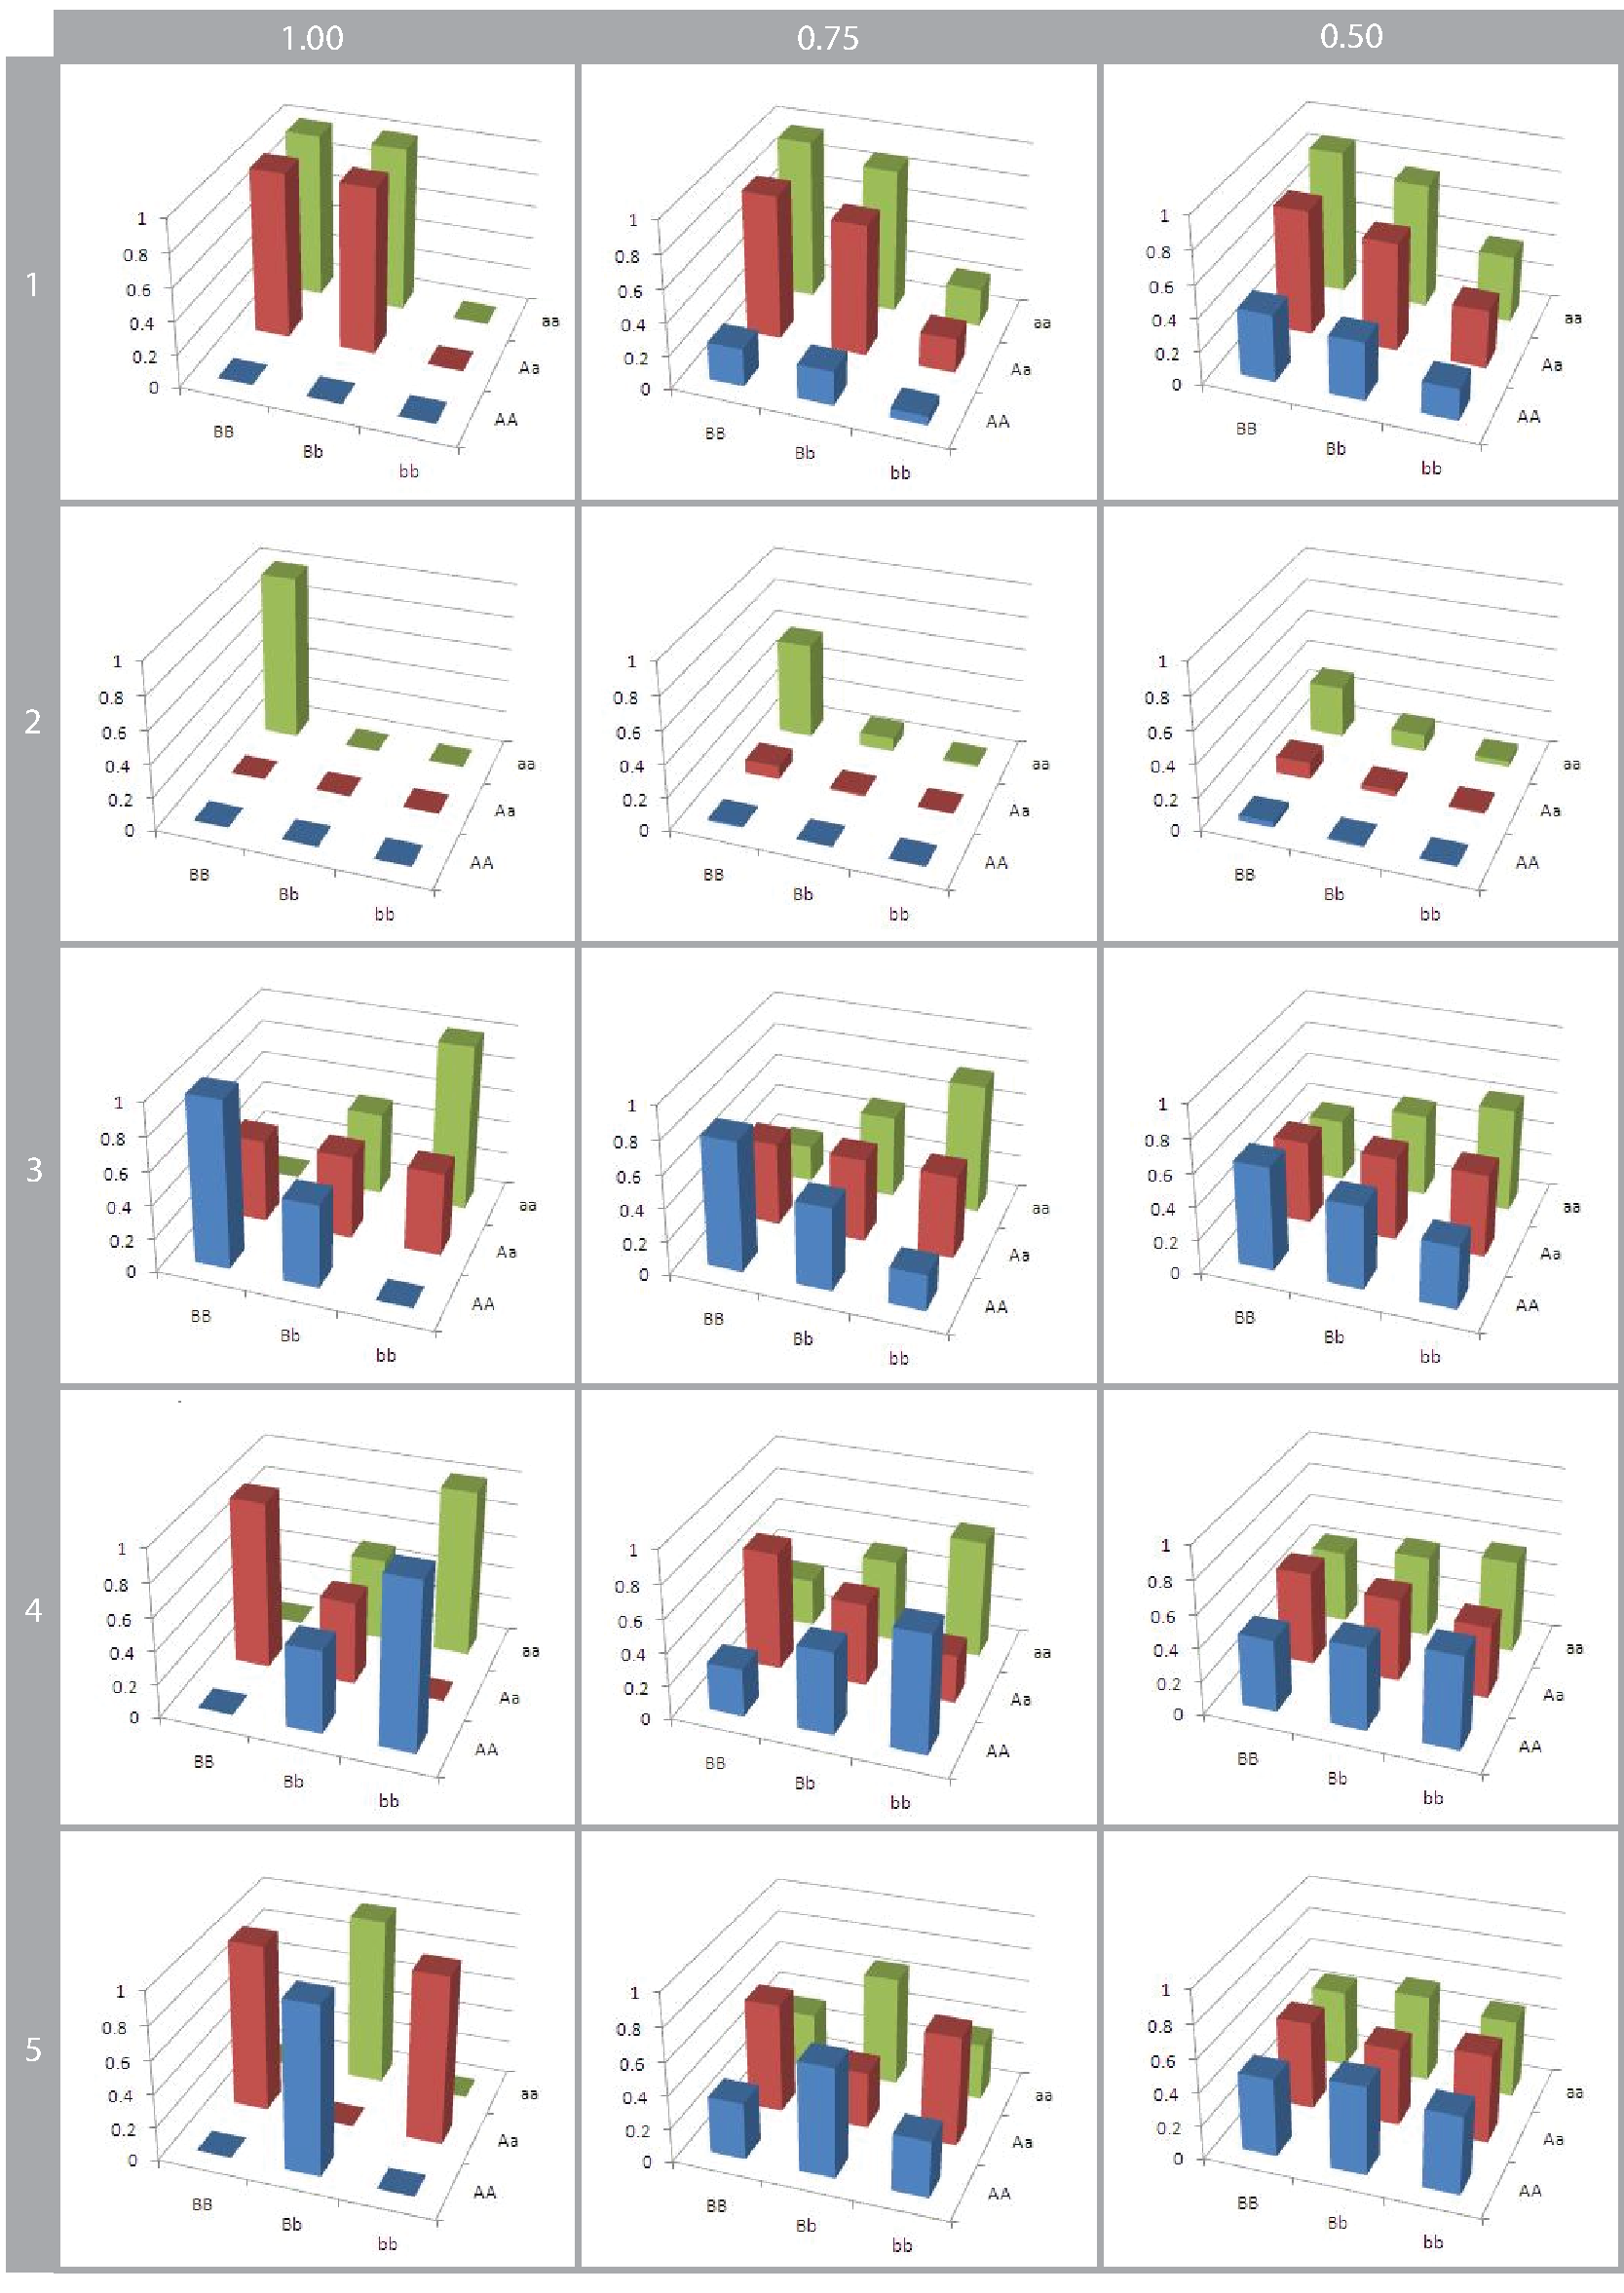
\includegraphics[width=4.5in]{Chapter4/gpmaps_ld.pdf}
\caption[Effect on LD on GP map estimation]{Different genotype-phenotype maps of causal variants (rows of graphs) deterministically calculated from neighbouring SNPs in different levels of linkage disequilibrium (columns of graphs). All SNP and causal variant frequencies are set to 0.5. Rows 1-2: Canalisation; 3: $A \times A$; 4: $A \times D$; 5: $D \times D$.}
\label{fig:gpmaps_ld}
\end{center}
\end{center}
\end{figure}

A general point that can be made from these observations is that a realistic understanding of the abundance and diversity of natural variation is strongly biased by the methods that are routinely employed for the detection of causal variants, particularly through genome-wide association studies. Using single SNPs as proxies for causal variants exposes these types of assays to the risk of missing most non-additive effects, while the few non-additive effects that might be detected are likely to be interpreted as additive. This chapter explores the potential of constructing haplotypes from phased SNPs to bridge the gap between causal variants and marker panels in searches for epistasis.


\subsection{Functional and evolutionary principles of haplotypes}

Haplotypes, strings of consecutive alleles that comprise chromosomal segments, have the property of encoding genetic information in the form in which they are inherited. This is in contrast to using raw SNP data because the loss of phase partially scrambles the information between SNPs. Maintaining the phase for analysis is intuitively useful because under certain scenarios the absence of a causal variant from a SNP panel may not necessarily preclude it from being accurately captured by the incomplete information available. For example, if the causal variant is an ancestral mutation then it will likely be unambiguously present on one or several haplotypes in the population and absent from the rest. Such segregation allows for the causal variant to be explicitly included in a statistical model, whereas relying on independent SNPs alone creates a model based on proxies that are incompletely correlated to the causal variant. The only way that informative segregation will not occur amongst haplotypes in this situation is through a double recombination event, or through a restorative mutation. Unfortunately, mutations that have arisen more recently are unlikely to segregate so informatively. For example, if the mutation occurred on a common haplotype then in the absence of a recombination event carriers and wild type individuals will be indistinguishable. In this case haplotypes are unlikely to confer an advantage over single SNPs, however neither approach is likely to be particularly powerful.

A second way in which haplotype parameterisations may have advantages over independent SNPs is through the implied inclusion of non-additive terms in the statistical models. By considering a string of alleles jointly, not only is each allele's independent effect being modelled jointly, but also included are all interactions amongst alleles, as well as the phase of the allele. As postulated in several publications (\emph{e.g.} \citealp{Haig2011}; \citealp{Schaid2004}; \citealp{Clark2004}), because haplotypes are functional units of genes, the tertiary structures that they ultimately form as proteins are directly related to the primary structures comprising those chromosomal segments. Interactions between non-synonymous mutations in these primary structures may be critical in protein folding, stability or function of the proteins and they are explicitly encoded as units of inheritance in the form of haplotypes. Such interactions could have interesting effects on the gap between pedigree-derived heritability estimates and those based on SNP-based relationship matrices in unrelated populations, because while the pedigree approach will consider the inheritance of a pair of interacting SNPs to be effectively a single additive allele, should low LD exist between those mutations then the SNP-based approach will fail to capture such terms when treating them independently. Indeed, many examples of such \emph{cis}-epistasis exist in the literature. They have been demonstrated in the human lactase gene \citep{Hollox2001}, human lipoprotein lipase \citep{Clark1998}, \emph{apoE} in association with cardiovascular disease \citep{Fullerton2000}, and for association between the risk of prostate cancer and the \emph{HPC2/ELAC2} gene \citep{Tavtigian2001}. In each of these cases haplotypes behave like `super alleles', explaining significantly more variation than the SNPs that comprise them do alone. In addition, other evolutionary features support the case for the existence of \emph{cis}-epistasis, such as population specific linkage disequilibrium clines of the major histocompatibility complex region \citep{Cavalli-Sforza1994} and the \emph{RET} region \citep{Chattopadhyay2003}. In general, statistical models become more complex when dealing with haplotypes because of the increased number of parameters, but as discussed in the following section this may be a reasonable trade off for an evolutionarily or biologically more realistic solution.


\subsection{Haplotype methods in current practice}

A wide range of haplotype association methods have been successfully developed for one dimensional scans. A convenient approach is to use a `sliding-window' framework. Here the haplotype test is sequentially applied to one fixed length of SNPs after another, with the `window' sliding to a new position (often one SNP at a time) after each test is performed. In general the window size is restricted to around 12 SNPs for two reasons, firstly the computational burden for haplotype methods often grows exponentially; and secondly, haplotypes that extend over long distances begin to incorporate SNPs in low linkage disequilibrium with the others. Thus chromosome structures are no longer represented, and extra parameters merely add noise. From a modelling point of view the advantages of haplotypes over independent SNPs (and even multiple SNPs considered jointly) are clear. However, from a statistical aspect and in a GWAS context it is slightly more ambiguous because there will always exist a trade-off between the variance explained by the model and the number of degrees of freedom used to explain it. Although many different methods have been published in the literature, there are ostensibly three main categories of haplotype testing: standard haplotype regression, haplotype clustering, and ancestral haplotype inference. These methods are discussed below.

It is technologically impractical to record haplotypes from DNA samples directly, rather single SNPs are typically measured independently with the heterozygotes among them having unknown phase, and haplotype reconstruction becomes a numerical problem. \cite{Excoffier1995} developed an expectation-maximisation (EM) algorithm that estimates haplotype frequencies in unrelated diploid populations, that were then applied in a case-control context through the construction of likelihood ratio statistics. This method has subsequently been adapted to quantitative traits by \citet{Powell2011} and \citet{Floyd2011}. In this context, the treatment of each haplotype is analogous to the treatment of an allele in an additive parameterisation of a multi-allelic ($>2$) marker. 

Because with the EM algorithm approach uncertainty generally exists as to an individual's true haplotype state at heterozygous markers, the $X$ matrix in the regression is encoded to be a set of quantitative features, with each parameter representing the sum of the probability of each individual having that haplotype at each chromosome. This approach does not include haplotype phase because there is no distinction made between opposing haplotype heterozygotes, but it will incorporate the \emph{cis}-epistatic interactions, in addition to potentially improving the association with untyped variants. An important breakthrough in phasing algorithms was developed by \citet{Kong2008}, which allows the rapid and accurate estimation of SNP phase over much longer distances through an entirely heuristic method. With the availability of tools that rapidly phase entire genomes using this method \citep{Hickey2011} it is now more computationally practical and statistically straightforward to employ haplotype-based methods in GWAS.

Particularly in the context of binary traits, a parallel cohort of methods exist that sidestep the issue of multiple degrees of freedom through clustering methods. An example of such a method was developed by \citet{Browning2006} in the form of the widely used {\tt BEAGLE} software \citep{Browning2007}. Here, rather than defining a fixed width window, a variable length markov chain is employed to grow the window size until a `sensible' haplotype block is defined, such that too many parameters in low LD are not included (reducing noise), and the model is not restricted to too few parameters in high LD (insufficient information content). A Fisher's exact test is then performed on the clustered haplotypes for case-control status. This method builds on several other similar clustering methods that use graphical models \citep{Thomas2005}, or hidden markov models \citep{Greenspan2004}, but has the advantage of adaptive window sizes and relative computational efficiency.

Another clustering approach is to exploit the evolutionary structure of haplotypes. \citet{Durrant2004} used a cladistic approach, whereby the inferred evolutionary history of the haplotypes of a particular window in the population are reconciled into a single rooted cladogram, with each branching point representing a time point where a new haplotype (or haplotype ancestor) arose. The inferred haplotypes at each time point are then tested for association with the trait. This multiplies the already high multiple testing penalty by the sliding window size, but for a one dimensional scan this will not impart a significant impact on the order of magnitude of multiple tests. Because the within-clade haplotypes are structured there is likely to be redundancy between the tests and a Bonferroni correction will be overly stringent, however the most robust way to estimate the effective multiple testing penalty, through permutation, may become computationally difficult. Nevertheless, even with the Bonferroni correction this evolutionarily cogent approach imparts significant power improvements over independent single SNP methods. Other methods that cluster based on ancestry also exist. \citet{McPeek1999}, for example, used a hidden markov model, and \citet{Zollner2005} used MCMC to sample from the space of possible coalescent paths. Although these clustering methods are generally designed with case-control studies in mind, they can be adapted for use on quantitative traits relatively easily. 


\subsection{Extensions to epistasis}

How can haplotype methods be extended to improve the power to detect epistatic variants? This simulation study tries to address the problem from two different angles. Ideally, a haplotype method, when employed for epistasis, should take into consideration the following attributes:
\begin{description}
\item[Computational efficiency] Haplotype methods tend to be computationally intensive, so one way to employ haplotypes in a computationally tractable manner would be to use a strategy where haplotype procedures can be implemented independently at each locus.
\item[Degrees of freedom] It is important to avoid a negating trade-off of increased association with causal variants against many extra degrees of freedom.
\item[Locus specific window sizes] If interacting loci are in independent genomic regions then it is unlikely that a single haplotype window size will perform best in both locations.
\item[Unsupervised learning] Using the response variable to inform haplotype procedures may result in an inflated false discovery rate.
\item[Multiple testing] Many haplotype methods designed for additive effects perform multiple tests per haplotype window (\emph{e.g.} \citealp{Durrant2004}). This is impractical for epistasis because the multiple testing penalty will increase quadratically, as will computational demand.
\item[Statistical interpretability] Translating haplotype parameters in order to reconstruct the underlying genotype-phenotype map is of particular importance for purposes of prediction and biological understanding.
\end{description}

The first approach attempts to fulfil all these guidelines. It uses a sliding window scan whereby unsupervised clustering is applied to the haplotypes in each window to reduce the high dimensional chromosomal segments to a binary vector that can then be treated as a single phased `latent SNP'. If this latent SNP has a higher correlation with the hidden causal variant than any individual SNP in the SNP panel, then theoretically an improvement in power will be achieved when applying to a two-dimensional `latent SNP' scan.

The second approach is quite different, as it uses haplotype information in the statistical models directly. One problem with haplotype information in an epistatic context is that it is analogous to a multiallelic genetic marker, in the sense that each diploid individual will have two haplotypes at a particular window of SNPs, and to encode this information one simply parameterises the test based on the additive effect of each haplotype. Thus, extending this framework to two dimensions to search for epistasis, it is impossible to parameterise for anything other than the $additive \times additive$ effects (thus ignoring the other 3 interaction terms, and restricting the search to a rather narrow range of possible epistatic effects). To parameterise for whole genotype effects, pairs of haplotypes are coded into a diploid state \citep{Schaid2004}, thus creating sliding windows of diplotypes. Two locus diplotypes are then synthesised to model for \emph{trans}-epistasis. The other major challenge is the number of degrees of freedom in each test. Naturally, such an encoding will lead to an explosion in the number of degrees of freedom, particularly in the general case where the interacting loci are unlinked. To overcome this a feature selection method is used to shrink the high dimensional design matrix to an optimum level of sparsity. Extensive simulations are performed to assess the potential benefits of such approaches over the single SNP method in a two-dimensional genome-wide context.

\section{Methods}

The simulations described here operate in a fairly standard manner, with the purpose of creating population-genomic scenarios where different tests can be applied and compared for their efficacy at detecting ungenotyped (or in the case of simulation, artificially `hidden') causal variants. For the parametric reduction methods (section \ref{sec:methods_supervised}) two chromosomes are simulated, and from these chromosomes a set of SNPs are chosen to be the SNP panel and a mutually exclusive second set of SNPs form a panel of QTLs to sample from. For various testing conditions a SNP is chosen from each chromosome to form an interacting QTL pair, and the SNPs comprising the SNP panel are used to scan for the absent epistatic interaction. A similar procedure is used for the clustering methods except all simulations are performed on a single chromosome in one dimension (section \ref{sec:methods_unsupervised}).

\subsection{Genome simulation}\label{sec:genome_simulation}

The two main methods for the simulation of population level genomic data, forward-in-time and coalescent based, have been widely compared \citep{Carvajal-Rodriguez2008, Cyran2008, DiVentura2006}. In general it is considered more computationally efficient to use coalescent approaches, but more evolutionarily accurate to use forward-in-time simulation. Of principle concern in this study is the evolutionarily realistic construction of haplotypes for a large number of individuals at sequence level resolution. To this end, the forward-in-time {\tt FREGENE} software tool \citep{Chadeau-hyam2008, Hoggart2007} was used. {\tt FREGENE} simulates the evolution of a monoecious, diploid single chromosomal population over non-overlapping generations, allowing parameters for mutation, recombination, and demographic and selection processes to be defined by the user. The simulation template involves a list of sites on the chromosome at which polymorphisms exist, such that a sequence level resolution of mutations in the population can be achieved. For this study two 20 megabase chromosomes were simulated over two rounds of evolution. First, for 300 generations, beginning from a `null' population with no diversity, with no recombination hotspots and all sites neutral. This was then repeated, but this time with the output from the first round comprising the base population for the second round.

A SNP chip comprising two chromosomes was generated from this output, with each chromosome comprising 6670 SNPs to achieve the effective density of a million SNPs across the genome ($\frac{1000000}{3000/20} \approx 6670$). SNPs were selected such that a uniform distribution of minor allele frequencies (MAFs) $\geq0.05$ comprised the panel. An exclusive QTL panel was also generated for each chromosome in the same manner, with the underlying frequency distribution also being uniform. SNP and QTL panels had no missing values, and phase was known.


\subsection{Methods in unsupervised haplotype clustering} \label{sec:methods_unsupervised}

An advantage of unsupervised machine learning methods is that by avoiding training the parameters with a response variable there is no inflation of the type I error rate, and there is no further increase in the multiple testing penalty. Both features are particularly desirable in the context of epistasis as the consequences of these issues are likely to hamper power quadratically. Here, clustering methods were applied to haplotype data with the purpose of reducing the large number of parameters involved in testing haplotypes to a binary vector that can be treated as a single `latent SNP'. If the clustered haplotype is more closely correlated with untyped causal variants than single SNPs in the panel then both the power of their detection and the accuracy of genotype-phenotype map estimation will improve. This hypothesis was tested using simulations where a single SNP in a SNP panel was selected as an unknown variant, and its correlation against other SNPs in the panel was compared against its correlation with clustered haplotypes.

So to clarify the intention of this approach, if a causal SNP is absent from the SNP panel in a GWAS, the ability to detect the true effect of the SNP is related to the maximum LD between the causal SNP and the observed SNPs. In the context of non-additive variance components, in particular higher order epistatic components, this dependence increases (figure \ref{fig:gpmaps_ld}). While single SNPs may be out-performed at capturing the variance of the causal variant by haplotypes, this is at the cost of many more degrees of freedom. This section seeks to employ unsupervised clustering methods to reduce haplotypes to binary variables. If these binary variables are more strongly correlated with the missing causal variants than single SNPs then both single and two dimensional GWASs will have improved power.

Many established unsupervised clustering methods exist for continuous data, but there are fewer available for categorical data, with many of those that do exist designed with a focus on specific scenarios that are not necessarily applicable to haplotype clustering.

\subsubsection{$k$-modes algorithm}

Perhaps the most widely used clustering algorithm is $k$-means. This takes a non-hierarchical, partitioning approach, such that for a set of continuous variables comprising the matrix $\mathbf{X}$, and a desired number of clusters $k$, the rows of $\mathbf{X}$ are grouped to form $k$ partitions, or clusters \citep{MacQueen1967}. Each row of $\mathbf{X} = \{X_1, X_2, ... , X_n \}$ is called an `object' (or in this case a haplotype), each element of the object $X_i = \{x_{i, 1}, x_{i, 2}, ... , x_{i,m}\}$ is termed an `attribute' (or a SNP allele), and each column of $\mathbf{X}$, $\{A_1, A_2, ..., A_m\}$, is an attribute of length $n$ (the total number of unique haplotypes in the sample). The basic objective is to cluster all of these objects into just $k < n$ classes, where the classification is performed by choosing some way to stratify objects according to some measure of similarity (or dissimilarity).

In the traditional $k$-means case, each object's distance from all other objects' distances are calculated to compose a $n \times n$ distance matrix $D$. Most commonly, the distance metric used is the Euclidean distance, such that $D$ is calculated by

\begin{equation} \label{eq:Dmatrix}
D_{i_{1}i_{2}} = d(x_{i_{1}, j}, x_{i_{2}, j})
\end{equation}
where
\begin{equation}
d(x_{i_{1}, j}, x_{i_{2}, j}) = \sqrt{\sum^{m}_{j=1} ( x_{i_{1}, j} - x_{i_{2}, j}} ) ^{2}.
\end{equation}

The clustering is then performed on $D$, such that given a hypothetical set of $k$ new objects, $\mathbf{Q}$, a matrix of size $k \times m$, the expression
\begin{equation}
\sum^{k}_{l=1} \sum_{X_{i} \in \mathbf{C}_l} d(X_i, Q_l)
\end{equation}
is minimised, where $\mathbf{C}_l$ is the set of objects in cluster $l$.

While this framework can be used as a reasonable approximation for nominal categorical variables, like those comprising haplotypes, the treatment of discrete values as continuous can have significantly detrimental impacts on the clustering accuracy. An alternative formulation, the $k$-modes algorithm, deals with some of the limitations directly \citep{Huang1998}. Firstly, $D$ is calculated using a dissimilarity measure, rather than a numerical function such as the Euclidean distance. The dissimilarity measure used here is simply
\begin{equation}
\delta(X_{i,l}, X_{j,l}) = \left\{
\begin{array}{cc}
0 &  X_{i,l} \neq X_{j,l}\\
1 & X_{i,l} = X_{j,l},
\end{array}\right.
\end{equation}
with $\delta(\cdot, \cdot)$ replacing $d(\cdot, \cdot)$ in equation (\ref{eq:Dmatrix}). This simply measures the number of mismatches between two haplotypes, if there are fewer mismatches then the haplotypes are more similar, and more likely to be clustered together.

Secondly, in $k$-means $Q_l$ is calculated to be the geometric centre of the objects within each cluster $\mathbf{C}_l$, and naturally this results in a set $\mathbf{Q}$ comprised of continuous attributes. Alternatively, $k$-modes calculates $Q_l$ to be the mode of the set of objects in $\mathbf{C}_l$, thus preserving the categorical meaning of each cluster.

Thirdly, the goodness-of-fit of the clusters in $k$-means is obtained by treating the attributes as continuous by estimating the within group sum of squared errors. However the $k$-modes formulation treats the attributes as categorical by instead using a frequency based minimisation, such that the clusters are optimal when the inequality is satisfied for all $j = \{1, 2, ..., m\}$ and where $q_{j} \neq c_{l,j}$:
\begin{equation}
f_{r}(A_{j} = q_{j} \mid \mathbf{X}) \geq f_{r}(A_{j} = c_{l, j}	 \mid \mathbf{X})
\end{equation}
where
\begin{eqnarray}
F_{r}(A_{j} = q_{j} \mid \mathbf{X}) = \frac{n_{q_{j}}} {n}, \\
F_{r}(A_{j} = c_{l,j} \mid \mathbf{X}) = \frac{n_{c_{l,j}}} {n}, \\
\end{eqnarray}
and $n_{q_{j}}$ and $n_{c_{l,j}}$ are the counts of allele $A_{j}$ in matrix $\mathbf{Q}$ and $\mathbf{C_{l}}$, respectively.

As the goal of the clustering is to reduce a large number of haplotypes to a single phased SNP, the number of clusters $k=2$. Clustering the $D$ matrix, even to only two clusters is NP-hard \citep{Aloise2009}, and the algorithm used, described in \citet{He2006}, is an iterative approximation whose results depend upon the randomly selected starting conditions. To avoid random artefacts, the algorithm is repeated five times, taking the best fitting clustering set as the solution. This is unlikely to be the optimal solution, and as is the nature of NP-hard problems it is difficult to validate the accuracy, but nevertheless it is a reasonable approximation \citep{He2006}.


\subsubsection{Modified ROCK algorithm}

Another approach for clustering categorical data is the ROCK algorithm \citep{Guha2000}. Developed to cluster categorical data from large scale market transactions, it addresses the problem where if there are a large set of possible categories, but each transaction chooses only a very small proportion of these, the similarity in all truly related transactions may be very low. Following the premise that while two transactions may have very few chosen items in common, a third transaction could share transactions with both of the first two, thereby linking them indirectly, the ROCK algorithm judges similarity not on pairwise distances, but extended to consider how many global \emph{links} between transactions exist.

While the translation to haplotype data is not immediately possible the concept applies well. For example, recent mutations are likely to generate divergent haplotypes, but these can be linked by recombination events to unify ancestral haplotypes. In its original form, the algorithm is concerned with how many of the chosen items from a large set of attributes are the same between transactions and uses the Jaccard similarity coefficient as the initial distance calculation, however with genotype data the informative value of each genotype allele is equal. For a window of $w$ phased SNPs from a sample of $2n$ chromosomes there will exist $m$ unique haplotypes, $\mathbf{H} = \{H_{1}, H_{2}, ..., H_{m}\}$, where $h_{1,...,w} \in \{0, 1\}$ such that $1$ represents the major allele, and $0$ the minor. A weighted distance matrix is calculated as
\begin{equation}
D_{ij} = \sum^{w}_{l=1}\gamma(H_{il}, H_{jl})
\end{equation}
where
\begin{equation}\label{eq:gammadist}
\gamma(H_{il}, H_{jl}) = \left\{
\begin{array}{cc}
0 &  H_{il} \neq H_{jl}\\
q & H_{il} = H_{jl} = 1\\
1 - q & H_{il} = H_{jl} = 0
\end{array}\right.
\end{equation}
where $q$ is the minor allele frequency of SNP $l$. Subsequently, a matrix of global relatedness $L$ is created first by reducing $D$ to a matrix of `links' such that
\begin{equation}
\tilde{D}_{ij} = \left\{
\begin{array}{cc}
0 & D_{ij} < \bar{D}\\
1 & D_{ij} \geq \bar{D}
\end{array}\right.
\end{equation}
where $\bar{D}$ is the mean of the values in the lower triangle of $D$, and then summing the number of `links' shared between each pair of haplotypes $H$,
\begin{equation}
L = \tilde{D}\tilde{D}.
\end{equation}
Thus $L$ is a symmetrical matrix, where the lower (or upper) triangle values represent the number of haplotypes that each haplotype pair have `links' with in common. Grouping into two clusters is then performed in the standard manner of the original ROCK algorithm, maximising values of $L$ within clusters whilst minimising between clusters, such that the most connected haplotypes are grouped together.


\subsubsection{Latent class modelling}

An established method for the reduction of categorical data into $k$ categories is the latent class model, which seeks to relate the set of discrete multivariate variables to a set of orthogonal latent variables (or clusters), such that for each of the $k$ clusters the probability of membership to each cluster is assigned to each individual. Here the output is continuous, and therefore unfeasible to apply as anything other than additive (or additive by additive etc.) genetic parameters. To overcome this problem each individual was clustered according to their estimated mode latent class (\emph{i.e.} the latent class with the highest probability). The theory is described in \cite{Goodman1974}, and the implementation used was from the R package {\tt R/e1071}.


\subsubsection{Cladistic clustering}

It is possible to treat the evolutionary history of the haplotype diversity in a sample more explicitly by inferring an evolutionary path from the hypothetical common ancestor to all contemporary haplotypes (those that exist in the data). A cladistic approach described by \cite{Durrant2004} attempts to do this, such that the haplotypes are clustered backwards in time through $w$ clades so at each time point increasingly diverse haplotypes are clustered together and individuals are assigned a new set of ancestral haplotypes. The authors use each time point's cluster as an independent test, thus increasing the genome wide multiple testing penalty by $w$. However, in terms of power such an approach is unfeasible when increasing the dimensionality of the search to include epistasis, so in this case only the oldest ancestral clustering sets ($k = 2$) are used. This is achieved by using the distance metric in equation (\ref{eq:gammadist}) in the construction of the $D$ matrix through the $k$-modes method.


\subsubsection{Simulation strategy} \label{sec:unsupervised_methods}

The accuracy and power of GWAS is, ostensibly, constrained by the correlation between unobserved causal variants and observed SNPs in the panel. The simulations in this study were composed to compare the efficacy of the unsupervised haplotype clustering methods against single SNP markers.

SNP panels were simulated for a single 20 megabase chromosome to have the effective density of 100k, 300k, 500k, 700k or 900k SNP chips, and for each QTL panels were generated such that the maximum minor allele frequency was limited to 0.1, 0.2, 0.3, 0.4 or 0.5 (the minimum frequency for all scenarios was 0.05, and frequencies were uniformly distributed). Therefore, 25 different genomic conditions were assessed.

For each genomic condition, 500 QTLs were drawn from the QTL panel, and the different clustering strategies were tested. For each haplotype clustering method a sliding window comprising $\{2, 4, ..., 12\}$ SNPs were tested at 11 positions flanking the QTL, such that the central two SNPs in the window flank the QTL at the $6^{th}$ position. Similarly 5 markers up and down stream in the SNP panel were tested for the single marker analysis (figure \ref{fig:1Dscan}). The haplotypes were clustered to biallelic variables (SNPs) as described above, and the $r^2$ with the causal SNP recorded for each sliding window. The maximum $r^2$ between the causal SNP and the individual SNPs in the SNP panel was also recorded.

\begin{figure}
\begin{center}
\includegraphics[width=5.5in]{Chapter4/1Dscan.png}
\caption[Simulation strategy 1D scans]{Simulation strategy for unsupervised haplotype clustering methods. Causal variants are selected from the QTL panel, and the flanking SNPs in the SNP panel comprise the search space. Searches are performed in one dimension, and while the range changes according the size of the sliding window, the number of tests remains the same (11 sliding windows per search). In the graphical example blue motifs represent tests based on a 2 SNP sliding window, red motifs represent a 6 SNP sliding window, and green circles represent tests based on single SNPs. The greyscale gradient of the flanking SNPs represents the expected increase in LD with the causal variant as distance decreases.}
\label{fig:1Dscan}
\end{center}
\end{figure}


\subsection{Methods in supervised parameter reduction} \label{sec:methods_supervised}

The object of clustering is to reduce high numbers of parameters into smaller groups of parameters. Supervised parameter reduction approaches the problem from a different perspective, as it actually \emph{eliminates} variables that are uninformative. As discussed earlier, it is theoretically beneficial to use haplotype information as they may capture the variance of hidden variants more accurately than single SNPs alone, but parameterising epistatic searches using haplotype encodings may only serve to restrict the scope of the test. Therefore, the full genotypic information of the haplotypes is utilised by encoding them as diplotypes. The resultant high number of parameters is then reduced by one of two methods, using penalised parameter reduction (LASSO), or treating the diplotypes as a single genetic variance components (REML). 

The power of these two methods are tested using through simulation against the standard approach of single marker based two-dimensional scans (as in the software implementations in chapter 3, using the 8 d.f. parameterisation), or against the raw diplotype parameters (with no parameter reduction applied, and therefore with very high degrees of freedom).

\subsubsection{Encoding phased SNPs into diplotype parameterisation}

For a three dimensional array, $\mathbf{X} \in \{0,1\}$, if $x_{isk}$ is the $s^{th}$ SNP for the $i^{th}$ individual on chromosome $k$, where $k=1$ represents the paternal and $k=2$ the maternal chromosomes, then haplotypes are classed into discrete, non-heirarchical categories that effectively take the binary sequence of alleles in the haplotype and convert into a base 10 integer:
\begin{equation}
u_{ik} = \sum_{s=1}^{w} x_{isk}2^{w-s}
\end{equation}
where $w$ is the SNP window size, $i = \{1, 2, ..., n\}$ where $n$ is the number of individuals, and the haplotype class $u \in \{1, 2, ..., 2^{w}\}$. With relatively high LD between adjacent SNPs in a window, as is natural in SNP panels, there will likely be many fewer haplotypes than the number of possible combinations, such that the number of observed haplotypes $p_{u} \leq 2^w$. The design matrix $U$ with dimensions $n \times p_{u} \times 2$ can then be constructed from $u$. Fitting haplotypes will essentially parameterise for additive terms, to incorporate the full genetic effect of a locus (including dominance) the model must parameterise for diplotypes. There are theoretically $2^w(2^w+1) / 2$ possible diplotypes for a window of length $w$, so for example in the two locus case where the first and second loci comprise diplotypes from 6 SNP windows each, there are $2^{12} \times (2^{12} + 1) / 2 = 8390656$ possible diplotypes. Naturally the actual number of diplotypes is limited by the number of individuals $n$, and when linkage disequilibrium exists between SNPs within a window then this number reduces significantly again. Each individual's diplotype can be coded from their haplotypes as
\begin{equation}
v_{i} = \left\{
\begin{array}{ll}
u_{i1} > u_{i2} & u_{i1}(u_{i1}+1) / 2 + u_{i2} \\
u_{i1} < u_{i2} & u_{i2}(u_{i2}+1) / 2 + u_{i1} \\
u_{i1} = u_{i2} & (u_{i2}+1)(u_{i2}+2) / 2 -1,
\end{array}\right.
\end{equation}
such that
\begin{equation}
q_{j} = \frac{1}{n} \sum^{n}_{i=1} v_{i} \cap j
\end{equation}
where $q_{j}$ is the frequency of the $j^{th}$ diplotype. This diplotype encoding strategy can be used for various supervised statistical strategies.


\subsubsection{Treating diplotypes as fixed effects}
\label{sec:dip_fixed}

The diplotype design matrix $V$, of size $n \times p_{v}$ where $p_{v}$ is the number of observed diplotypes, is constructed for standard least squares regression such that the first column is $V_{.1} = \mathbf{1}^n$, and for the remaining columns $j = \{2, 3, ..., p_{v}\}$
\begin{equation}
V_{ij} = \left\{
\begin{array}{ll}
v_{i} = j & q_{j} \\
v_{i} \neq j & 1 - q_{j}.
\end{array}\right.
\end{equation}

The effect of each diplotype, treated as fixed, is then calculated through ordinary least squares
\begin{equation}
\mathbf{\hat{b}} = (\mathbf{V^{T}V})^{-1}\mathbf{V^{T}y}
\end{equation}
and analysis of variance is performed to obtain a $p$-value for the $F$-test
\begin{equation}
\left (
  \frac{1}{p_{v} - 1} \sum^{n}_{i = 1} (\hat{y}_{i} - \bar{y})^{2} 
\right )
\left (
  \frac{1} {n - p_{v}} \sum^{n}_{i = 1} (y_{i} - \hat{y}_{i})^{2}
\right )^{-1}
\sim F(p_{v}-1, n - p_{v})
\label{eq:ftest}
\end{equation}
where
\begin{equation}
\mathbf{\hat{y}} = \mathbf{\hat{b}V}
\end{equation}
and $\bar{y}$ is the mean of $y$.


\subsubsection{LASSO regression}
\label{sec:dip_lasso}

Of principal concern with performing fixed effects analysis with diplotypes is the large number of degrees of freedom employed to explain what is expected to be a very small proportion of the phenotypic variance. Ostensibly the power of such an approach is unlikely to be particularly high when analysed using ordinary least squares. One approach to overcome this problem is to use shrinkage methods that will reduce the $\mathbf{V}$ matrix to a sparse subset of parameters $\mathbf{V^{*}}$. LASSO regression (least absolute shrinkage and selection operator) is one such method that is widely used \citep{Tibshirani1996}. As a regularisation method, its objective is to perform feature selection without overfitting. The danger of overfitting in this case is that the data will effectively inform the hypothesis, inflating the probability of rejecting a true null hypothesis. LASSO achieves regularisation by constraining the coefficients with an $\mathcal{L}^{1}$-Norm, such that the ordinary least squares estimate

\begin{equation}
\hat{\beta} = \underset{\beta}{\operatorname{argmin}} \sum^{n}_{i=1} \left ( y_{i} - \alpha - \sum^{p_{v}}_{j=1} v_{ij} \beta_{j} \right )^2
\label{eq:lasso1}
\end{equation}
is constrained subject to 
\begin{equation}
\sum^{p_{v}}_{j=1} | \beta_{j} | \leq t
\label{eq:lasso_constraint}
\end{equation}
where $\hat{\beta}$ is the LASSO estimate and $t \geq 0$ is a tuning parameter. Such a procedure is useful in this context because it has the value of reducing a very large number of diplotypes to a much smaller subset of relevant diplotypes without bias, thus avoiding an inflation in the type I error rate while potentially increasing the power of the test. Equations \ref{eq:lasso1} and \ref{eq:lasso_constraint} can be reconciled for direct calculation as
\begin{equation}
\hat{\beta} = \underset{\beta}{\operatorname{argmin}} \left \{ \sum^{n}_{i=1} \left ( y_{i} - \alpha - \sum^{p_{v}}_{j=1} v_{ij} \beta_{j} \right )^2 + \lambda \sum^{p_{v}}_{j=1} | \beta_{j} | \right \}
\end{equation}
where $\hat{\beta}$ is the LASSO estimate and $\lambda \geq 0$ is a tuning parameter such that when $\lambda = 0$ then the LASSO estimate is identical to ordinary least squares, and $\hat{\beta} = \mathbf{\hat{b}}$. Otherwise, as lambda increases the parameters with the smallest coefficients are dropped from the model, and the remaining coefficients shrink towards 0. The entire shrinkage path can be calculated efficiently via coordinate descent using the {\tt R/glmnet} package \citep{Friedman2010}. Ultimately, a set of $n_{\lambda}$ estimates of $\hat{\beta}$ are made for $\Lambda = \{\lambda_{1}, \lambda_{2}, ..., \lambda_{n_{\lambda}} \}$, such that 
$\mathbf{\hat{B}} = \{ \hat{\beta}_{1}, \hat{\beta}_{2}, ..., \hat{\beta}_{n_{\lambda}} \}$. Ordinarily, to select the set of coefficients to be fitted in the final model $k$-fold cross validation is performed, using the element of $\Lambda$ that minimises the mean squares error. However, for the sake of computational efficiency this was approximated by choosing the value of $\Lambda$ that minimised the residual sum of squares,
\begin{equation}
\lambda^{*} = \underset{\lambda \in \{1, ..., n_{\lambda} \}}{\operatorname{argmin}} \sum^{n} (\mathbf{y} - \mathbf{V\hat{\beta_{\lambda}}})^2,
\end{equation}
thus the regularised least squares estimate can then be tested in the standard manner as in equation \ref{eq:ftest}, where $\hat{y}$ is replaced by
\begin{equation}
\hat{y}^{*} = \mathbf{V}\hat{\beta}_{\lambda^{*}}
\end{equation}
and the term $p_{v}$, the number of degrees of freedom denoting the number of parameters in the model, is replaced by
\begin{equation}
p^{*}_{v} = \sum^{p_{v}}_{j=1} \hat{\beta}_{\lambda^{*}j} \neq 0.
\end{equation}


\subsubsection{Random regression using REML}
\label{sec:dip_reml}

As an alternative to fitting each diplotype parameter as fixed effects, they can be treated as random effects that compose a single genetic variance component. This potentially circumvents the problem of high dimensionality in terms of statistical power, as an analysis of variance can be performed that treats the variance component as a single degree of freedom.

The random diplotype effect is tested for significance in a standard unbalanced random effects model. For the $i = \{1, 2, ..., p_{v} \}$ diplotypes in the sample, and $n = \sum^{p_{v}}_{i=1} n_{i}$ individuals, where $n_{i}$ is the number of individuals with the $i^{th}$ diplotype, the ragged matrix 
\begin{equation}
Y_{ij} = \begin{pmatrix}
y_{1,1}	& 	y_{1,j}	&	\cdots	&	y_{1,n_{1}} \\
y_{i,1}	&	y_{i,j}	&	\cdots	&	y_{2,n_{2}} \\
\vdots	&	\vdots	&	\ddots	&	\vdots \\
y_{p_{v},1} &	y_{p_{v},2} &	\cdots	&	y_{p_{v}, n_{p_{v}}}
\end{pmatrix}
\end{equation}
where $y_{ij}$ is the $j^{th}$ individual with the $i^{th}$ diplotype, is modelled as
\begin{equation}
Y_{ij} = \mu + U_{i} + W_{ij}
\end{equation}
where $U_{i}$ is the random effect of the diplotypes and $W_{ij}$ is the individual-specific error. Restricted maximum likelihood (REML) estimates of the variances for these terms, $\tau^{2}$ and $\sigma^{2}$ respectively, are made and these using the {\tt R/lme4} package, and can be tested for significance using a one degree of freedom F-test by
\begin{equation}
\frac{\sigma^{2} + n_{0} \tau^{2}}{\sigma^{2}} \sim F(1, n_{0}-1)
\end{equation}
where
\begin{equation}
% [ 1 / (k-1) ] * [ N - sum (n_i)^2 / N ]
n_{0} = \frac{1}{p_{v} - 1} \left (n - \frac{1}{n}\sum^{p_{v}}_{i = 1} n_{i}^{2} \right ).
\end{equation}

\subsubsection{Simulation strategy}

The object of these simulation is to test the performances of the different methods under varying conditions of epistatic patterns, genetic variances and genomic architectures in the context of two-dimensional exhaustive scans.

\begin{itemize}
\item Two patterns of canalisation and $additive \times additive$, $additive \times dominance$ and $dominance \times dominance$ patterns were simulated ($N_{P} = 5$, figure \ref{fig:gpmaps_ld}).
\item Each pattern was simulated such that they explained $V_{G} / V_{P} = H^{2}$ = \{0.5\%, 1\%, 2\%, 3.5\%, 5\%\} of the phenotypic variance, $N_{H^{2}} = 5$.
\item Genomic architecture varied according to
\begin{itemize}
\item Number of individuals = \{1000, 2000, 4000\}, $N_{n} = 3$.
\item QTL minor allele frequencies were uniformly distributed, with maximum frequencies = \{0.1, 0.2, 0.3, 0.4, 0.5\}, $N_{Q} = 5$.
\item Effective SNP chip density = \{100000, 300000, 500000, 700000\}, $N_{D} = 4$.
\end{itemize}
\end{itemize}
Enumerating all combinations listed above there are $N_{P}N_{H^{2}}N_{n}N_{Q}N_{D} = 1500$ different `scenarios' in total. Using the two simulated chromosomes (section \ref{sec:genome_simulation}), for each scenario 100 `causal variants' were sampled from each QTL SNP panel and a phenotype was simulated corresponding to the conditions of that scenario. The SNPs in the SNP panel that neighbour the sampled QTLs were then tested for association with the simulated phenotype using the following methods:
\begin{itemize}
\item Standard 8 d.f. standard pairwise test of association
\item Diplotypes of window size = \{2, 4, 6\} at each chromosome treated as fixed effects (section \ref{sec:dip_fixed})
\item Diplotypes of window size = \{2, 4, 6\} at each chromosome fitted using the LASSO method (section \ref{sec:dip_lasso})
\item Diplotypes of window size = \{2, 4, 6\} at each chromosome treated as random effects (section \ref{sec:dip_reml})
\end{itemize}
Each method/window size combination was treated as an independent `scanning method' ($3\times3+1=10$ scanning methods). Four neighbouring windows for each chromosome were scanned, such that for each causal variant a $5 \times 5$ neighbouring grid was scanned for association with the simulated phenotype and maximum $p$-values were recorded for each scan (figure \ref{fig:2Dscan}).

\begin{figure}
\begin{center}
\includegraphics[width=5.5in]{Chapter4/2Dscan.png}
\caption[Simulation strategy 2D scans]{Simulation strategy for supervised haplotype reduction methods. Causal variants are selected from the QTL panel from each chromosome, and the flanking SNPs in the SNP panel comprise the search space. Search grids change in size depending on the 2D sliding window size, but the number of tests per search remain the same ($5 \times 5 = 25$). Examples of search grids for $2 \times 2$ (red) and $4 \times 4$ (blue) SNP sliding windows are shown. As in figure \ref{fig:1Dscan} the greyscale gradient of the flanking SNPs represents the expected increase in LD with the causal variant as distance decreases.}
\label{fig:2Dscan}
\end{center}
\end{figure}

In addition to the above, for each causal variant simulated at each scenario a null test was also performed, such that all conditions remained the same except the genetic variance was set to 0. The distribution of $p$-values from these null models were used to generate thresholds based on false discovery rates for each scanning method, from which estimates of power can be made.


\section{Results}

\subsection{Unsupervised haplotype clustering}
\label{sec:unsupervised_haplotype_clustering}

Incomplete LD between causal markers and observed SNPs results in the rapid decay of estimated genetic variance, the misrepresentation of genotype-phenotype maps, and a prohibitory reduction in statistical power of detection (figure \ref{fig:gpmaps_ld}). To rescue this incomplete LD, unsupervised clustering methods were applied to haplotype data, and the large number of haplotypes were clustered into two groups to artificially create a binary variable that could be treated as a `latent SNP' in a (one or two dimensional) GWAS, with the hope that the it would be more highly correlated with unobserved causal variants than single SNPs in the SNP panel.

\begin{sidewaysfigure}
\begin{center}
\begin{center}
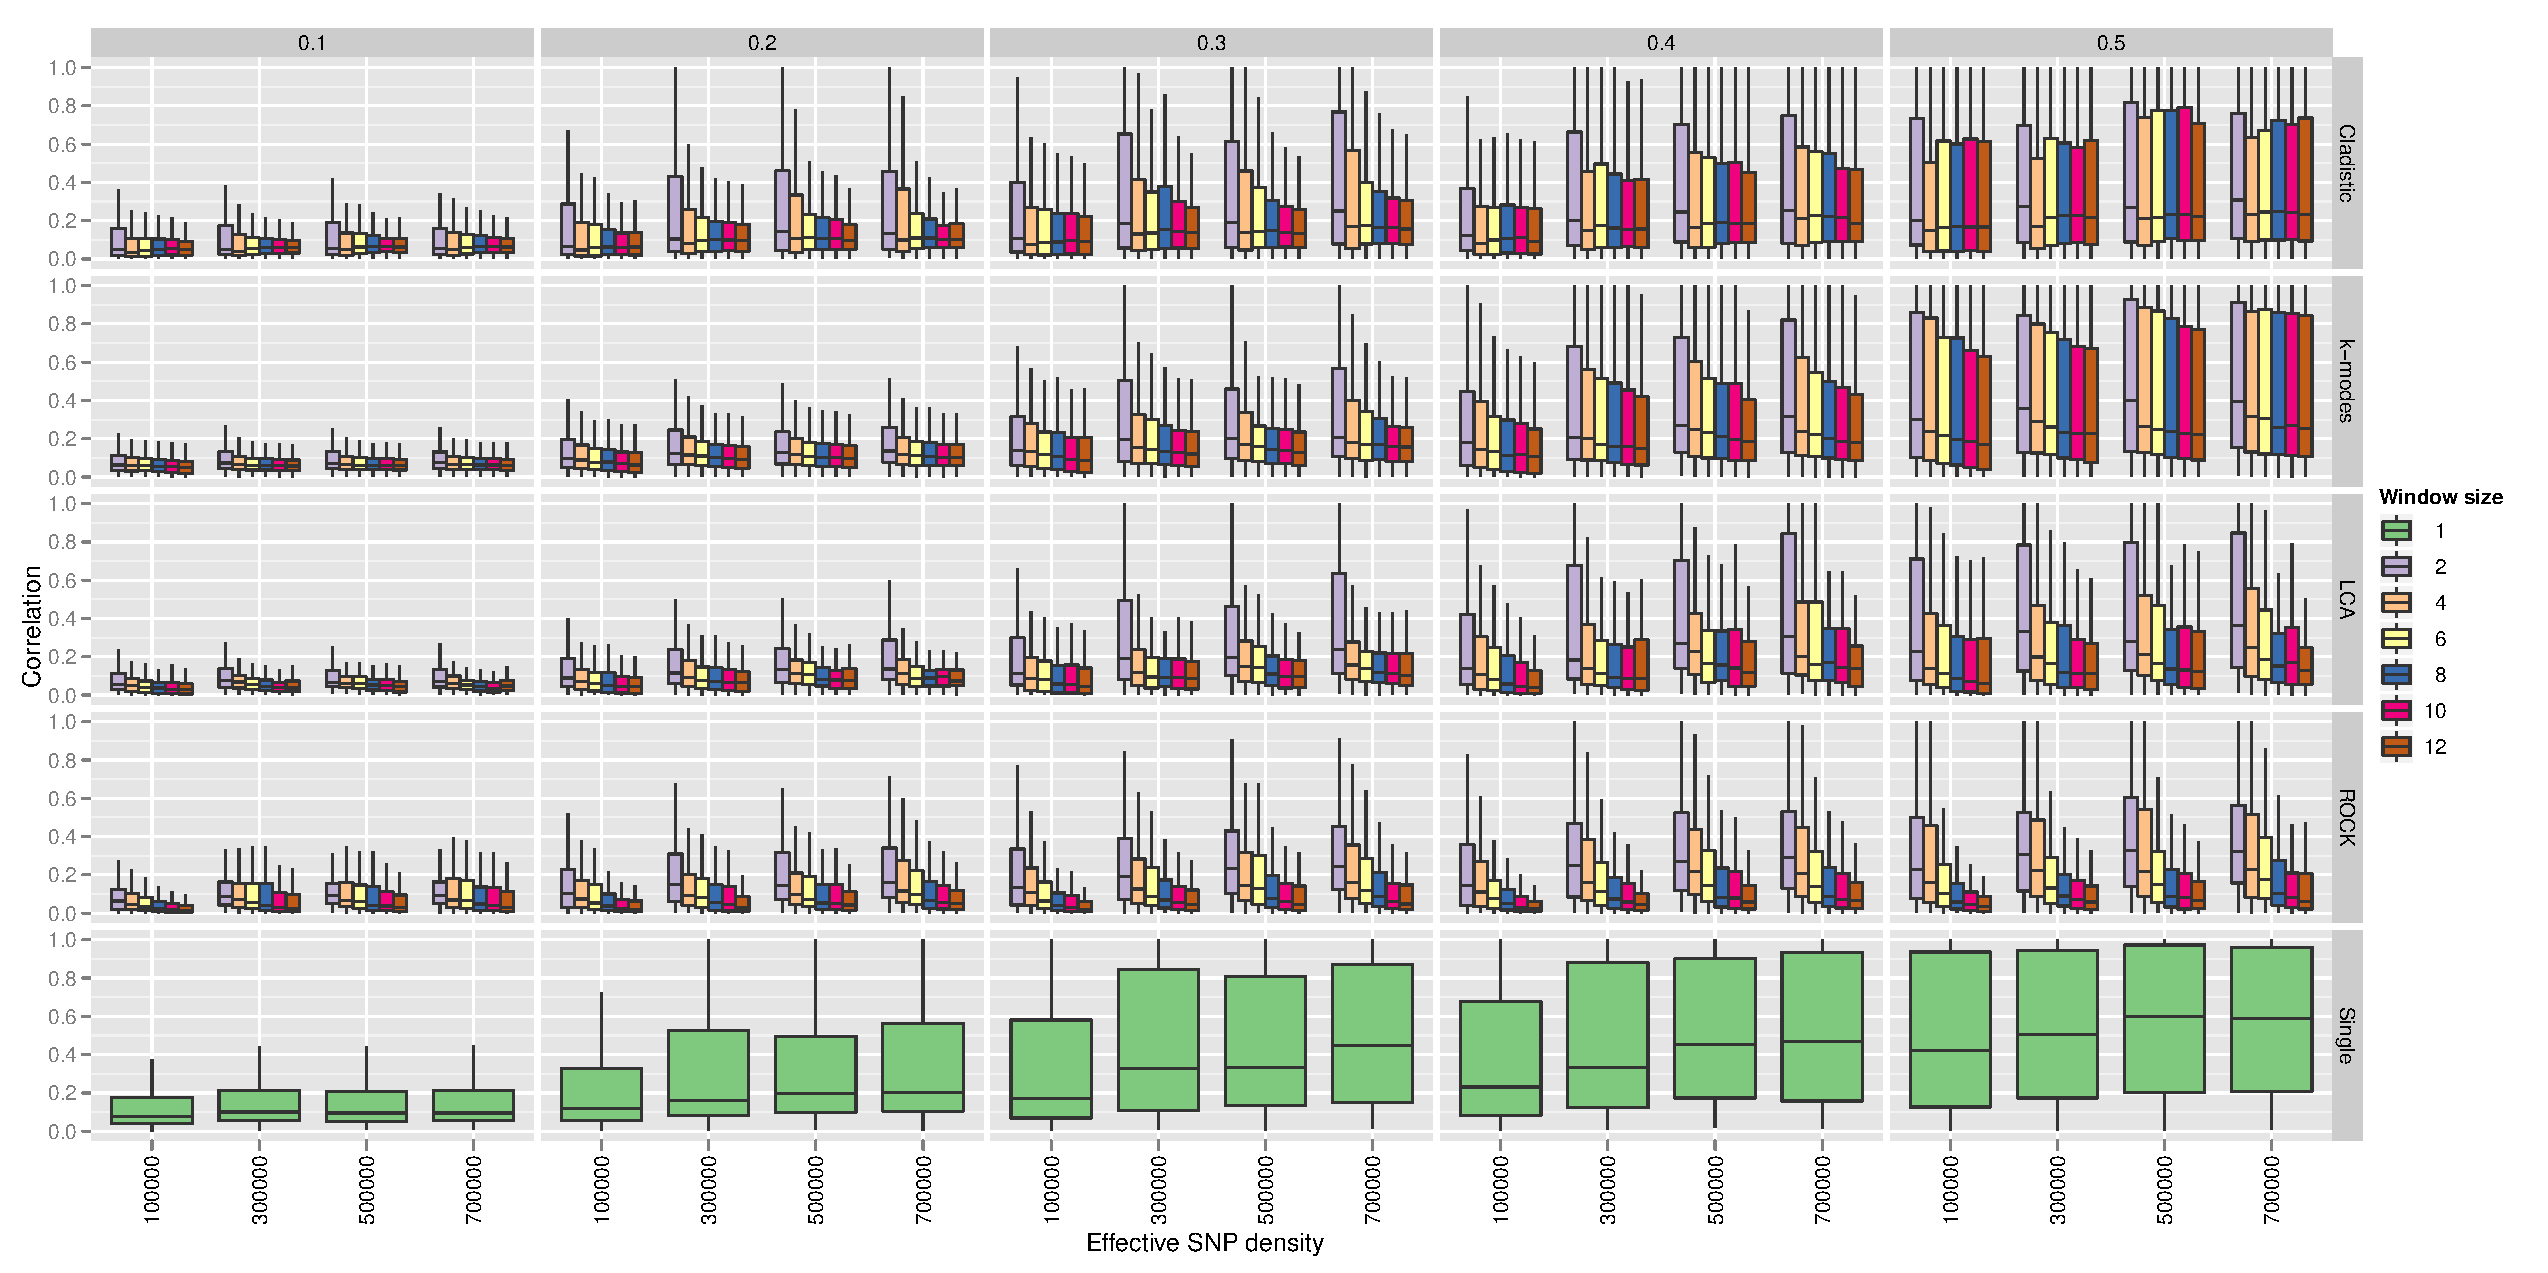
\includegraphics[width=8in]{Chapter4/compare_all_raw.pdf}
\caption[Detection of hidden variants using unsupervised haplotype clustering]{Detection of `untyped' causal variants in different genomic architectures. Box and whisker plots show the distribution of best correlations between causal variant and clustered SNPs (rows 1-4) or single SNPs (row 5), for different causal variant frequency distributions (columns of boxes), and different SNP chip densities ($x$ axis). Each distribution comprises 500 simulated causal variants. Box and whisper plots represent, from top to bottom, $95^{th}$, $75^{th}$, $50^{th}$, $25^{th}$ and $5^{th}$ percentile values for the distribution of correlation values.}
\label{fig:unsupervised_overall}
\end{center}
\end{center}
\end{sidewaysfigure}

The overall results of this simulation are shown in figure \ref{fig:unsupervised_overall}. There is no single clustering approach that captures the variance of untyped causal variants as consistently as simply using neighbouring single SNPs. A general trend can be seen across all methods of improved detectability as SNP panel density increases and as the distribution of causal variant frequencies becomes more similar to the distribution of SNP frequencies. While there is variation between the performances of different clustering methods, there is a tendency for haplotypes generated from smaller window sizes to perform better.

To assess the possible gain in detectability that could be achieved from the haplotype methods, the window size with the highest correlation with the causal SNP for each haplotype method was recorded. Figure \ref{fig:best_scenario} shows how much improvement in correlations could be gained if all window sizes were tested, including single SNPs, against using single SNPs alone. The ROCK algorithm has the best performance, and in particular when the distribution of frequencies of causal variants is most dissimilar to the distribution of SNP frequencies the largest gain is seen. While some extreme improvements are observed, the vast majority are fairly small, and it is unlikely that the increased multiple testing incurred would be offset by the performance gain, even in a one dimensional GWAS context.


% For discussion
% - biggest improvement where QTL frequencies are low - yang et al.
% - multiple testing is also used in durrant cladistic approach for 1D scans
% - SVM does not inform window size choice


\begin{figure}
\begin{center}
\begin{center}
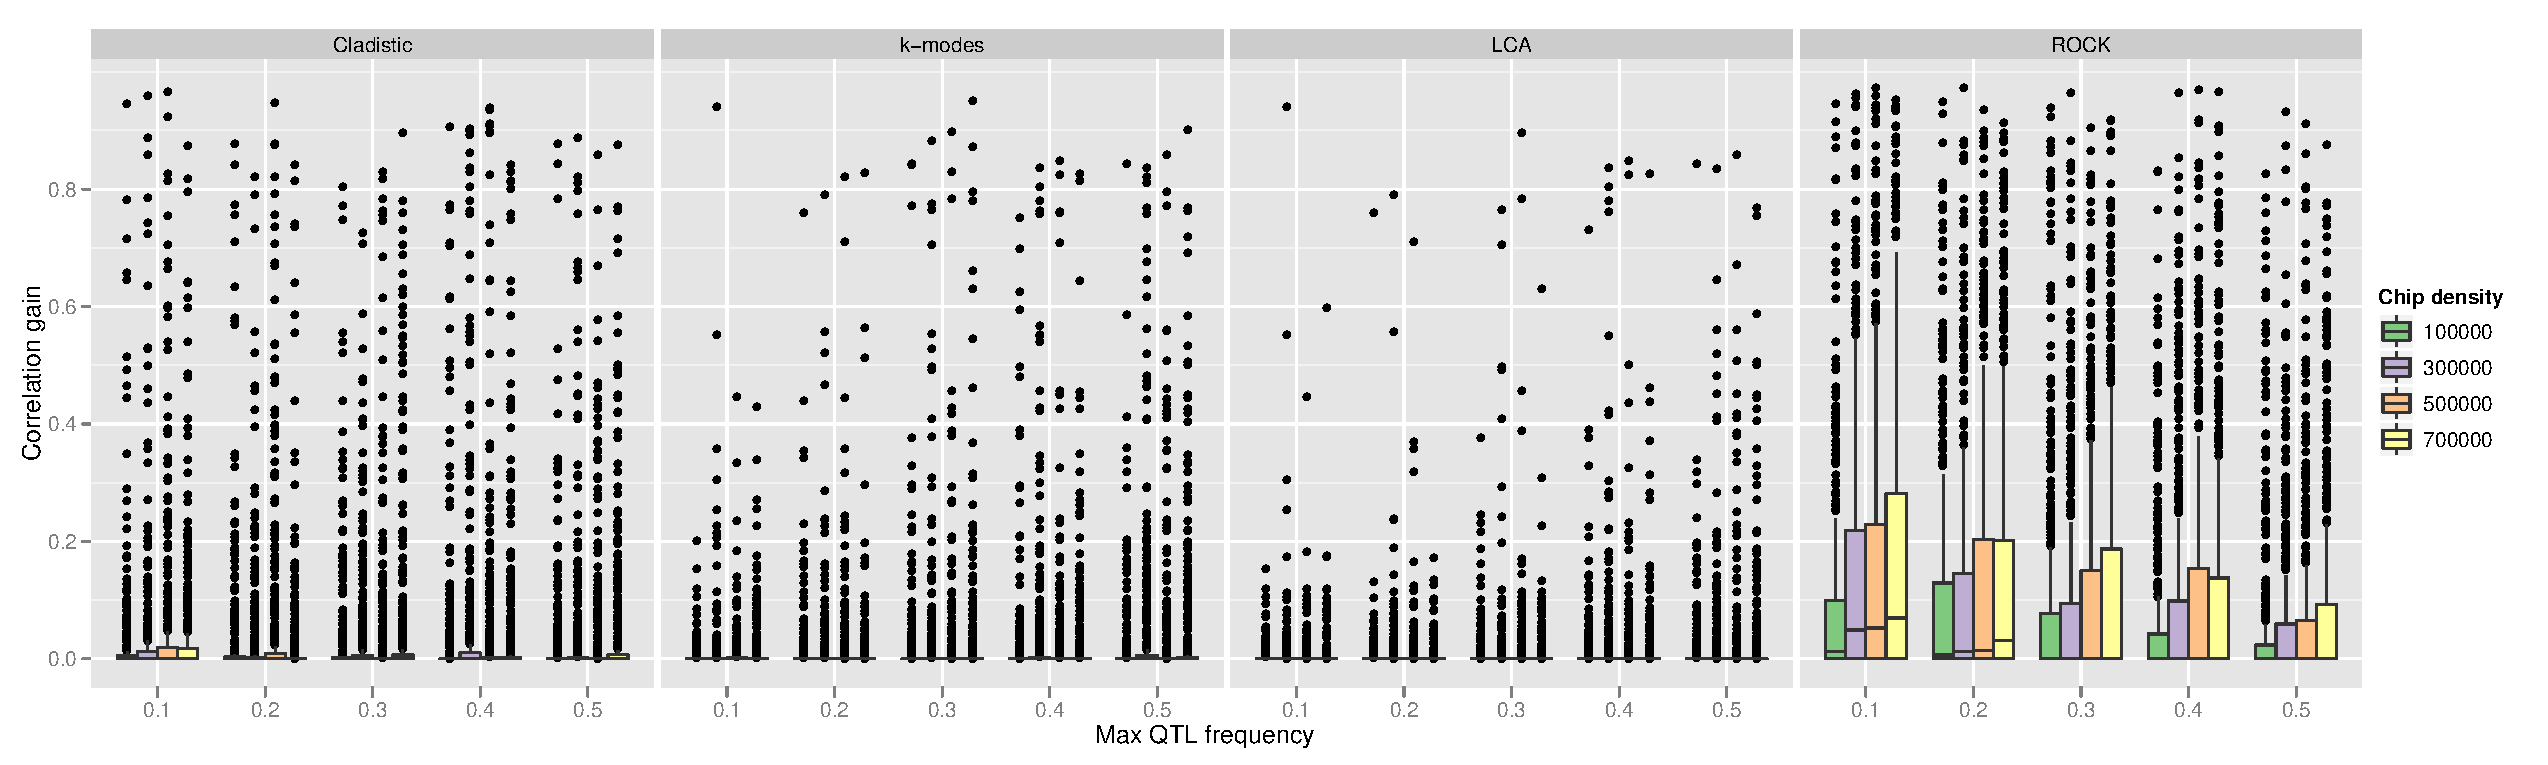
\includegraphics[width=5.5in]{Chapter4/best_scenario.pdf}
\caption[Maximum improvement in variant detection using unsupervised methods]{The improvement in correlation ($y$ axis) with `untyped' causal variants compared to single SNPs when using the `best' window size for a particular haplotype clustering method in a particular QTL setting. Boxes represent different clustering methods, and the frequency of causal variants is plotted against the $x$ axis. Box and whisker plots show the quartile bounds of 500 simulations, with midlines representing the median, whiskers representing the $95^{th}$ percentile value, and points representing outliers.}
\label{fig:best_scenario}
\end{center}
\end{center}
\end{figure}

\subsection{Supervised parameter reduction}

Overall the results from the simulations showed quite clearly that in almost all situations the power to detect epistatic associations was significantly improved by using the LASSO regression method on $2 \times 2$ sliding window diplotypes. This performance is sustained for most epistatic patterns and all tested genomic architectures, and power improvements are particularly pronounced when the genetic variance of the causal variants is lowest, approximately in the range that is likely to exist in real studies. The results are dissected in more detail below.

\subsubsection{False discovery rates for different methods}

% FDR as a function of Test, Window, N, Density
% Distributions of p-values for lasso 2
% Thresholds for power

The power of a scanning method, the rate of true associations discovered, can be calculated in a frequentist context through the use of thresholds. These thresholds are developed to impose a low family-wise false discovery rate, such that in practice, on a background of high multiple testing, the false positive rate is kept to some arbitrary low level. Because the different scanning methods employ varying methods that train parameters to the response variable, and then proceed to test the trained parameters for significance, it is possible that false discovery rates will vary and that different thresholds should be considered for different methods. Of particular concern is the LASSO, where although the feature selection process is regularised to avoid false positive inflation, the $\lambda$ selection step could risk the problem of using the data to inform the hypothesis test.

\begin{figure}
\begin{center}
\begin{center}
\subfigure[Test statistics from null models]{\label{fig:fdr_pvals}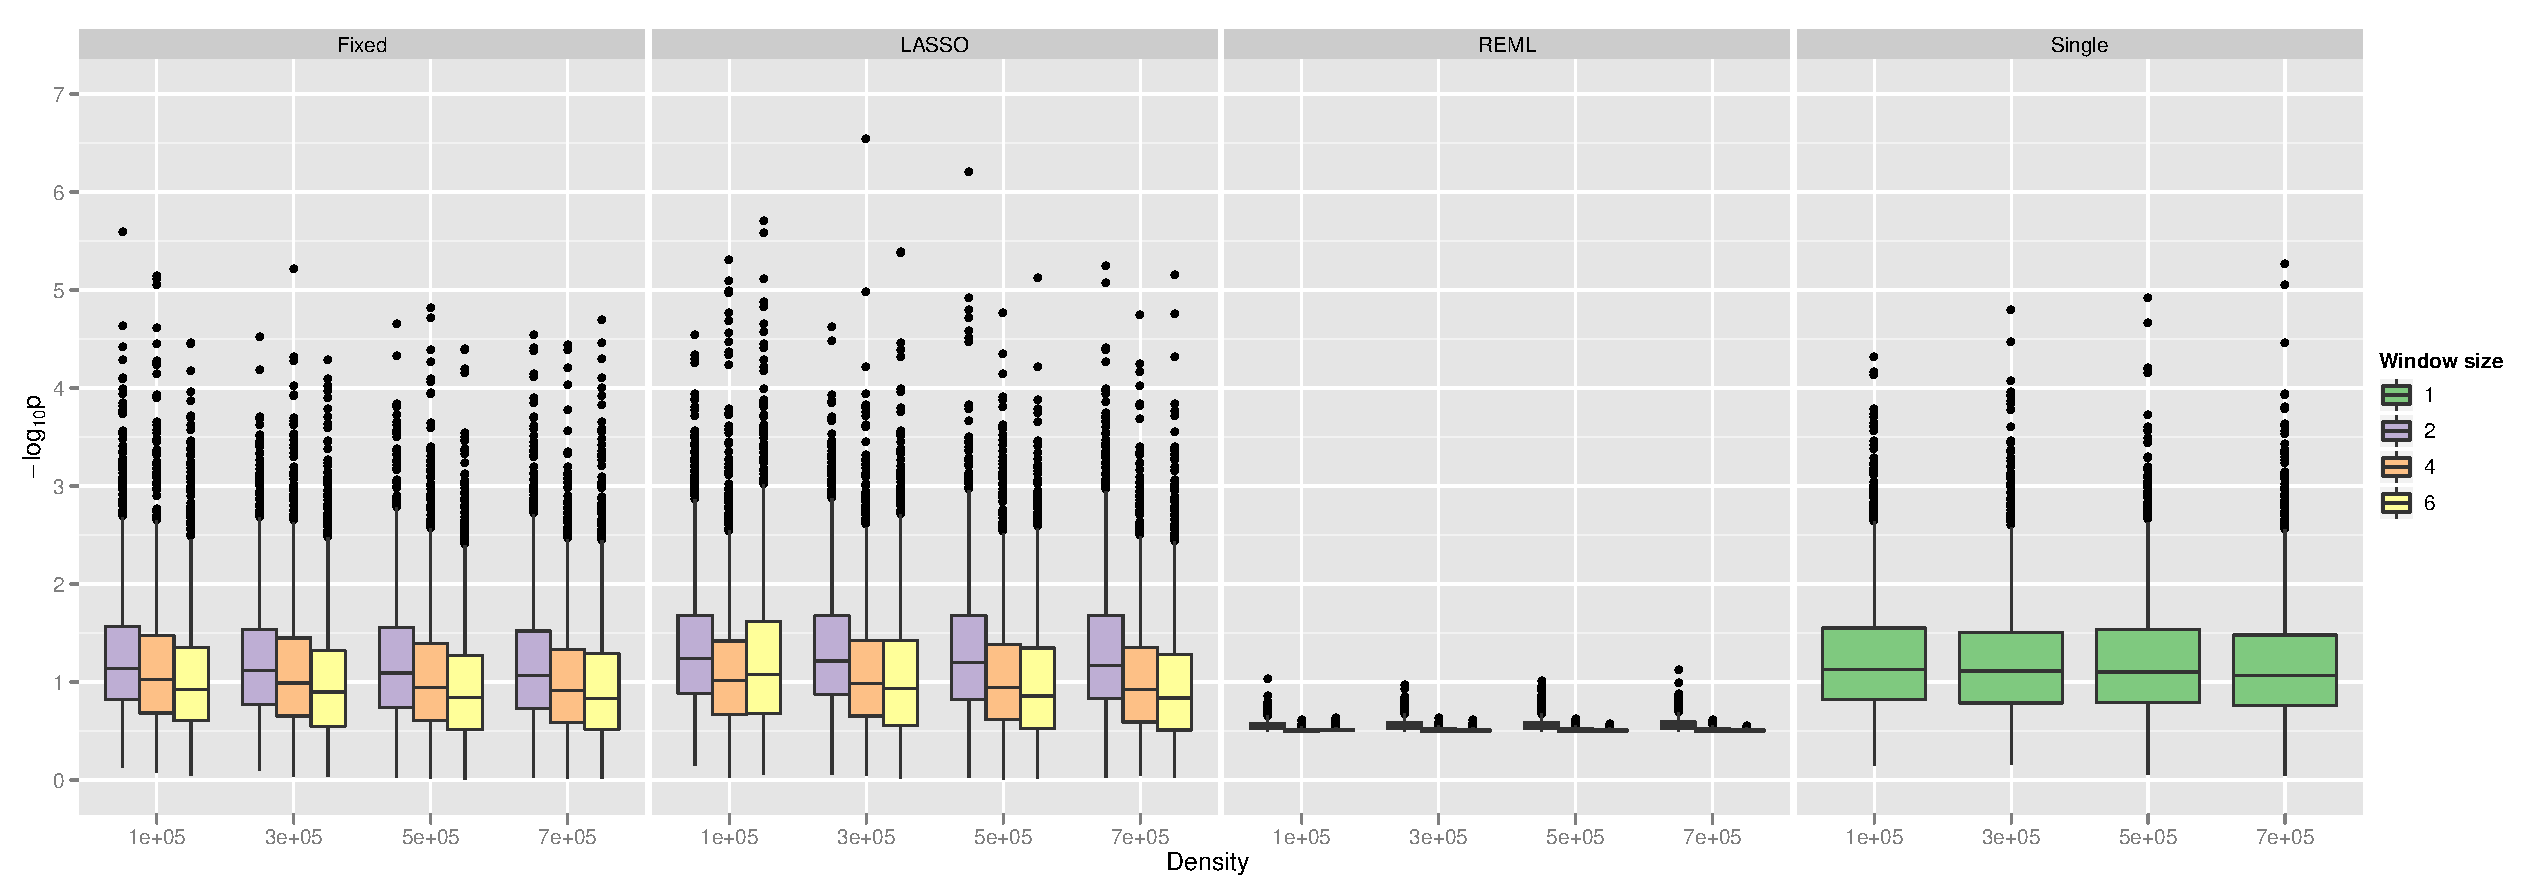
\includegraphics[width=5.5in]{Chapter4/fdr_pvals.pdf}} \\
\subfigure[Distribution of null $p$-values for LASSO]{\label{fig:fdr_lasso}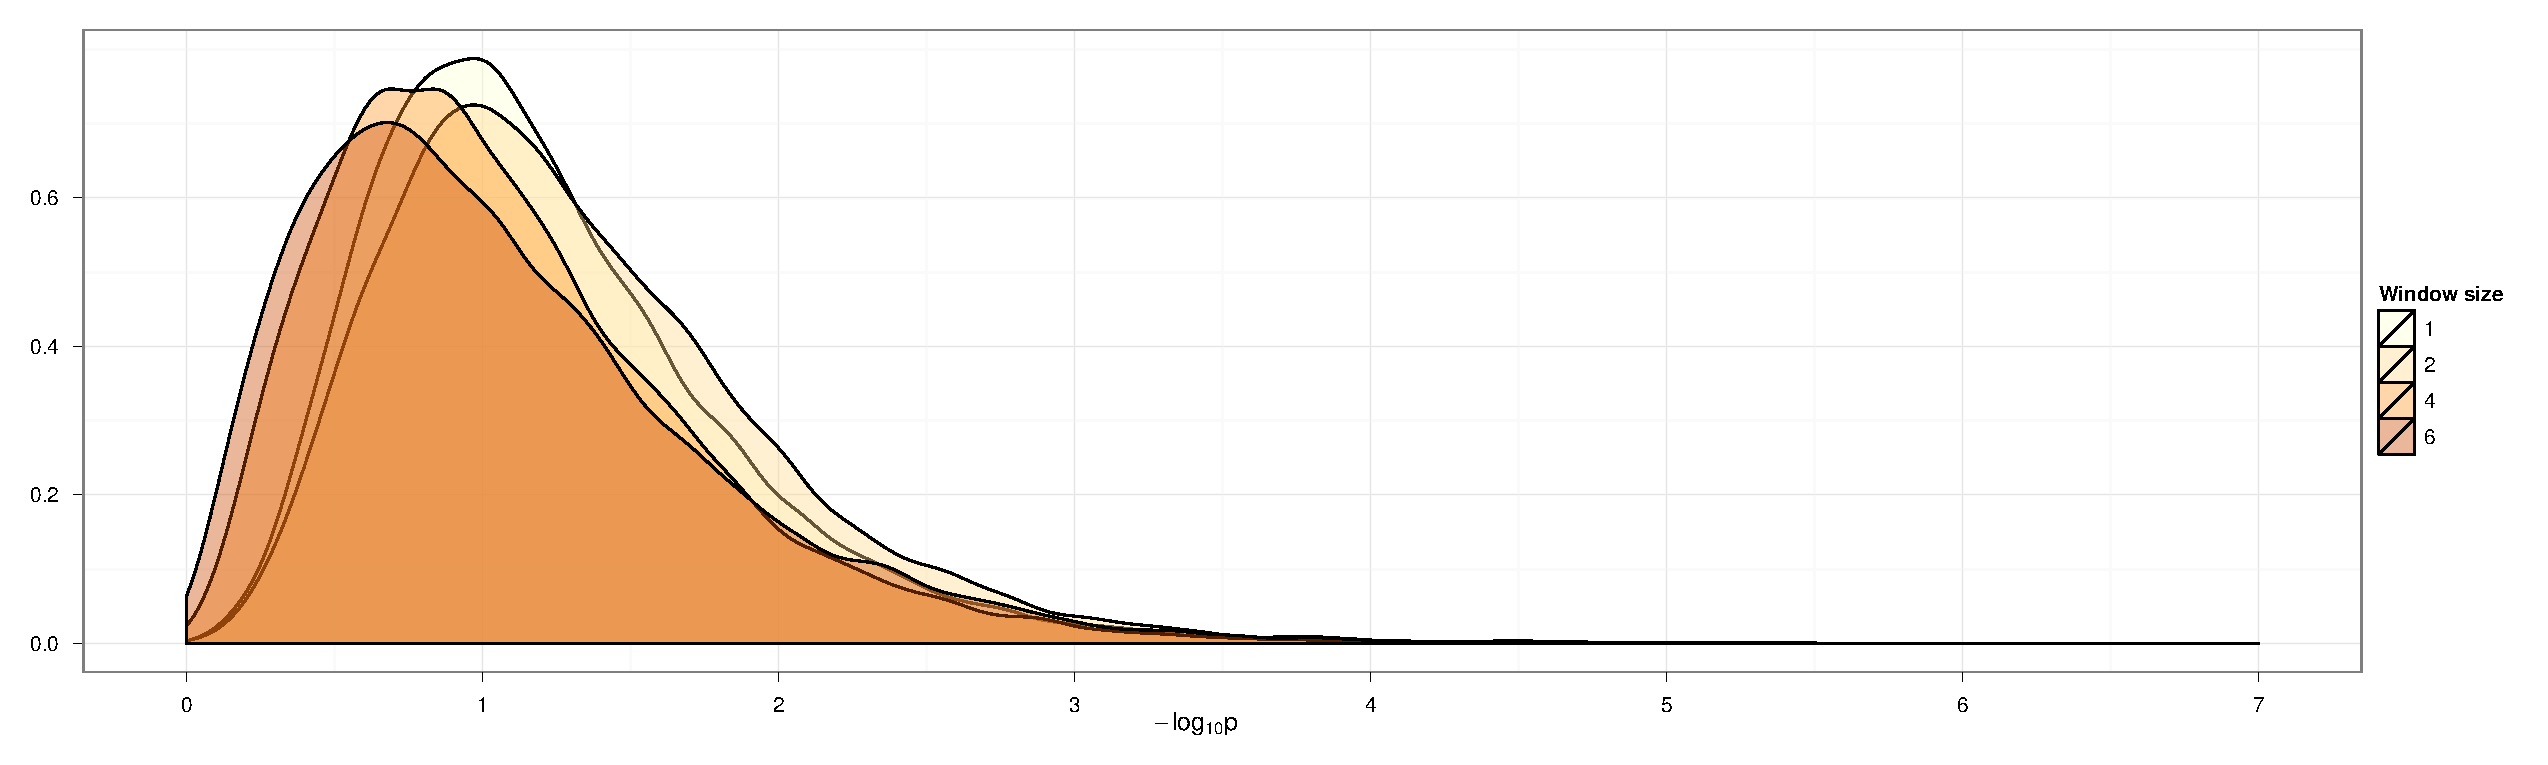
\includegraphics[width=5.5in]{Chapter4/fdr_lasso.pdf}} \\
\caption[False discovery rates for supervised methods]{(a) Box and whisker plots to show the distributions of $-\log_{10}p$-values for different scanning methods. Results are faceted by Test (large boxes), sliding window size (coloured boxes), and effective SNP chip Density ($x$-axis) as these factors had an impact on the distributions ($p < 0.05$). (b) $-\log_{10}p$ value densities for single SNPs (window size = 1) and different scanning window sizes for the LASSO method (windows 2, 4 and 6). Values are taken from simulations with effective SNP density of 500000. The sample size did not have a significant effect.}
\label{fig:fdr}
\end{center}
\end{center}
\end{figure}

For each scenario a repeat was performed where $H^{2} = 0$. A distribution of $p$-values from these null models was collated (figure \ref{fig:fdr_pvals}). The effective SNP chip density has a small effect on the distributions of all scanning methods. This is logical because as density decreases the effective number of independent multiple tests increases. For LASSO regression using $6 \times 6$ sliding window sizes this effect is more pronounced because as LD decreases the number of diplotypes increases, such that as $p_{v} \to n$ the LASSO shrinkage allows $(\mathbf{\hat{y}} - \bar{y}) \to (\mathbf{y} - \bar{y})$. As such the false discovery rate is inflated. However, in general there is relatively little difference between the fixed effects methods. $-\log_{10}p$ values from random effects estimates are, however, much lower. This could be partly due to most of the REML variance estimates converging at 0 for the null models.

The tails of the distributions are of principal concern for calculating thresholds for power estimation. While figure \ref{fig:fdr_pvals} shows that the median values of $p$-values are strongly affected by the sliding window size, closer examination of the distributions in figure \ref{fig:fdr_lasso} suggests that the tails are not so disparate. Correspondingly, the 0.05\% family-wise false discovery thresholds used for the power analysis are shown in table \ref{tab:thresholds}. Overall the impact of window size is very small.

\begin{table}
  \begin{center}
  \rowcolors{4}{tableShade}{white}
  \begin{threeparttable}
  \caption{\label{tab:thresholds}Thresholds calculated from 0.5\% false discovery rate}
    \begin{tabular}{llcccc}
    \toprule
Density \tnote{a} & Test	&	\multicolumn{4}{l} {Window size} \\
\cline{3-6} \noalign{\smallskip}
	& &	1	&	2	&	4	&	6	\\
\midrule
100000 & Single	&	3.45	& 	-	&	- 	&	-	\\
& Fixed   & - & 3.39 & 3.27 & 3.28 \\
& LASSO  &  - & 3.75 & 3.36 & 4.94 \\
& REML    & - & 0.78 & 0.58 & 0.72 \\
\midrule
300000 & Single& 3.29 &  - &  - &  - \\
& Fixed   & - & 3.35 & 3.46 & 3.23 \\
& LASSO  &  -& 3.60 & 3.48 & 3.82 \\
& REML &    - &0.80 & 0.59 & 0.66 \\
\midrule
500000 & Single & 3.33 &  - &  - &  - \\
& Fixed   & - & 3.53 & 3.09 & 3.12 \\
& LASSO  &  - & 3.80 & 3.23 & 3.27 \\
& REML   &  - & 0.84 & 0.60 & 0.61 \\
\midrule
700000 & Single & 3.45  & - &  - &  - \\
& Fixed   & - & 3.44 & 3.11 & 3.08 \\
& LASSO  &  - & 3.59  & 3.23 & 3.07 \\
& REML   &  - & 0.83 & 0.60 & 0.59 \\
\bottomrule
\end{tabular}
\begin{tablenotes}{\footnotesize 
\item[a] Effective SNP density}
\end{tablenotes}
\end{threeparttable}
\end{center}
\end{table}

\subsubsection{Power comparison of scanning methods}

% Power vs VarSim, colour = Test, grid = Pattern ~ Window size

There are many dimensions to the analysis under which causal variants were simulated and different testing methods were employed, comprising varying genotype-phenotype maps, QTL frequency distributions, SNP densities, sample sizes, genetic variance of QTLs and diplotype window sizes. Ultimately there was very little interaction between these facets, and so analysis of each factor is considered independently below.

\paragraph{Window size choice for diplotype methods}
Prior knowledge of the best window size to use for haplotype methods is difficult to ascertain. While perfect knowledge of the best window size would likely improve association performance, as in figure \ref{fig:best_scenario}, for the supervised methods on diplotypes considered in this section there is a clear demarkation in performance between different window sizes (figure \ref{fig:power_windows}). So for the remainder of the analysis only $2 \times 2$ SNP sliding windows are employed for the diplotype methods as they have a clear advantage over other window sizes.


\begin{figure}
\begin{center}
\begin{center}
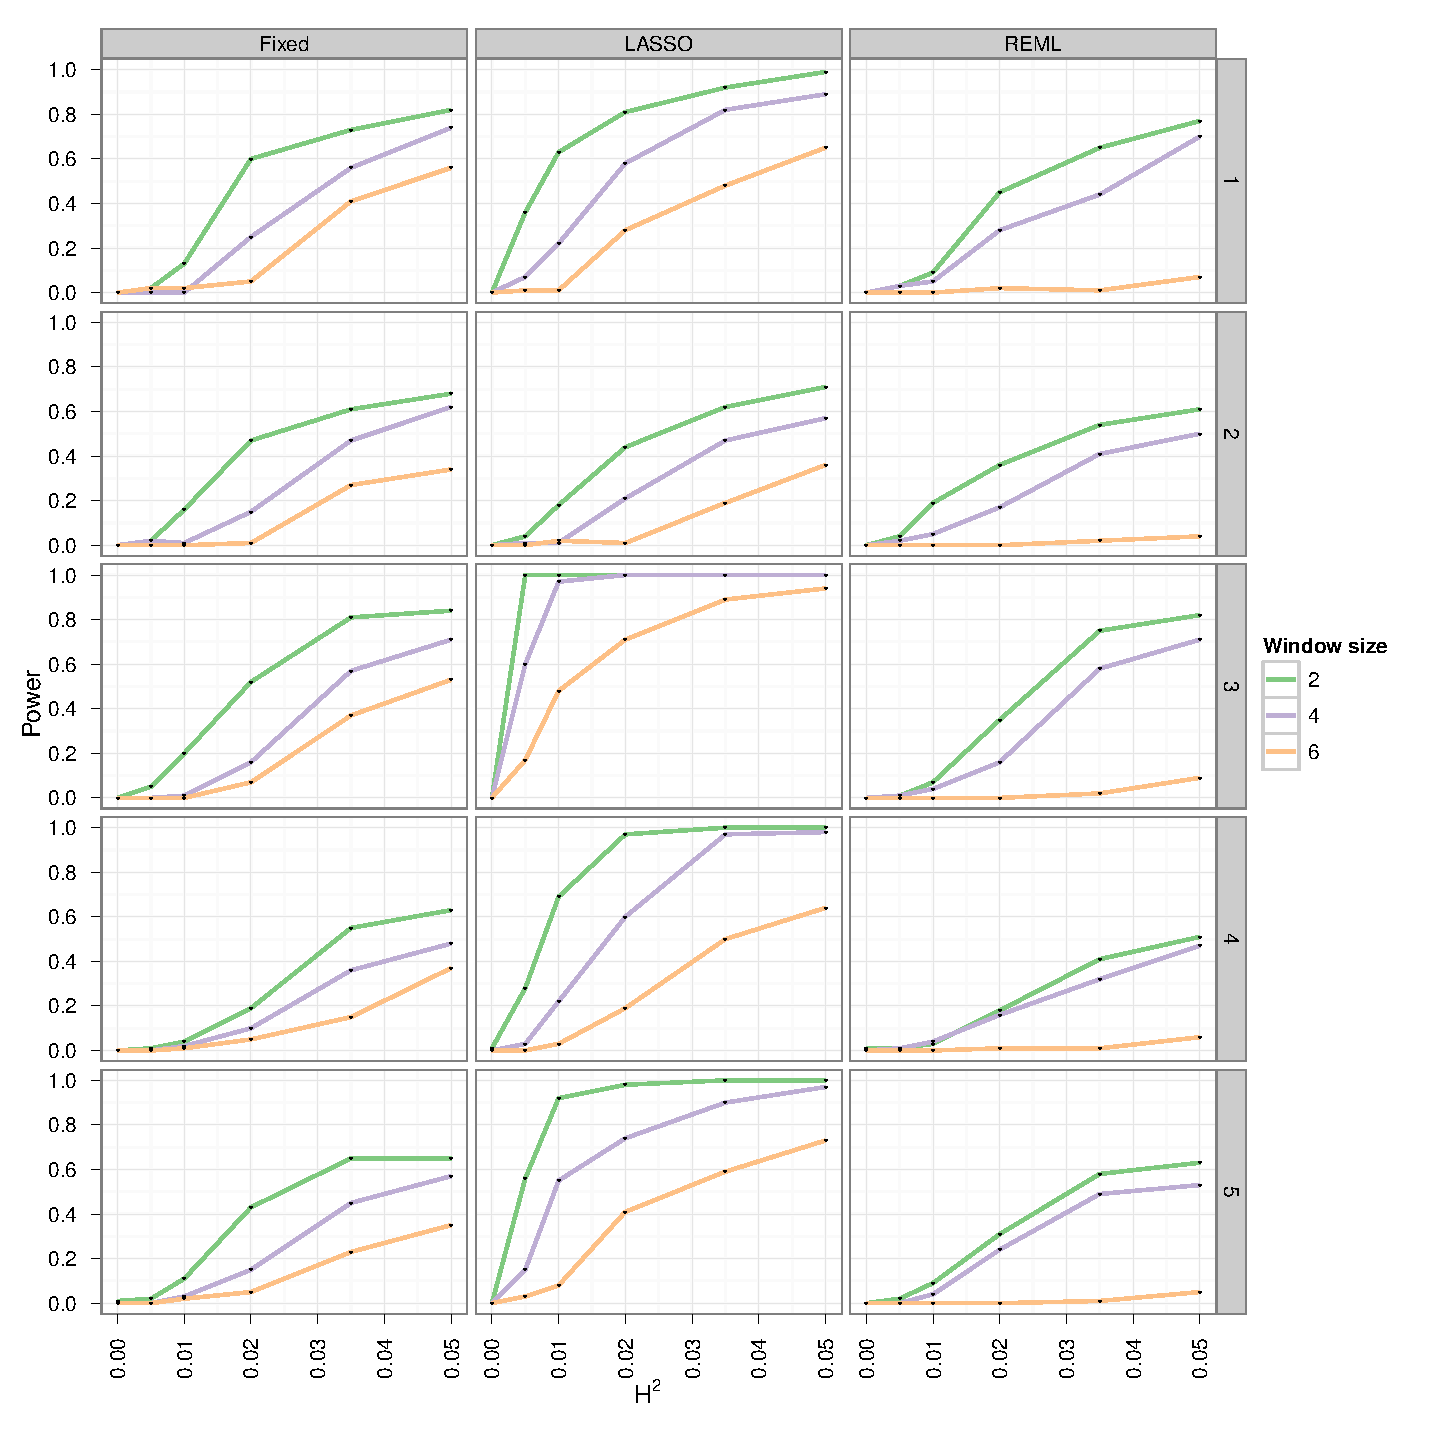
\includegraphics[width=5.5in]{Chapter4/power_windows.pdf}
\caption[Effect of window size on power of supervised methods]{Comparison of power between different window sizes (coloured lines) for each diplotype based test (columns of graphs). Rows of boxes represent different epistatic patterns correspond to genotype-phenotype maps in figure \ref{fig:gpmaps_ld} (first column, $r^2 = 1$).
\label{fig:power_windows}}
\end{center}
\end{center}
\end{figure}



\paragraph{Overall comparison of power for different genotype-phenotype maps}
Figure \ref{fig:power_methods} shows the power comparisons between the different diplotype methods and the single SNP method. A significant gain in power from using the LASSO method can be observed for four of the five genotype-phenotype maps simulated. Simulations involving genotype-phenotype map 2 (figure \ref{fig:gpmaps_ld}, column 1, row 2) appear to be the only scenarios where the LASSO method does not comprehensively outperform the other methods. As observed in previous results ($e.g.$ chapter 2, and \citet{Marchini2005} and \citet{Evans2006}), the widely variable properties of different genotype-phenotype maps makes it difficult to identify a single statistical framework that reliably outperforms others in all situations. One surprising observation is that the LASSO method performs extremely well for genotype-phenotype map 3 (figure \ref{fig:gpmaps_ld}, column 1, row 3), the $additive \times additive$ parameterisation. There is no obvious reason for this to happen as the diplotype design does not specifically parameterise for this pattern, and there doesn't seem to be anything peculiar about his pattern compared to the others. Further investigation may be required in this direction.

Treating the diplotype parameters as fixed effects with no shrinkage generally performs poorly compared to using single SNPs. While such methods have been successful when parameterised as haplotypes searching for additive effects, the exponential increase in parameters when expanding to epistasis is unlikely to be counterbalanced by a corresponding increase in variance explained over single SNP methods. Treating the diplotypes as random effects is a more intuitive approach to avoid the problem of high degrees of freedom, yet the performance is poor compared to all other methods. One possible problem with this method is that inaccurate variance estimates will be made when certain diplotype classes comprise of single or few individuals.

The magnitude of power for all methods drops when changing from an FDR based threshold (figure \ref{fig:power_methods_fdr}) to a Bonferroni based threshold (figure \ref{fig:power_methods_bonferroni}) that assumes a multiple testing penalty from an exhaustive two dimensional search. Generating a corresponding FDR would be computationally impossible, so it is assumed that for the LASSO and single SNP methods the tails of the distributions of $p$-values from the null models will be the same. Under these assumptions the qualitative result remains the same, in that LASSO regression on diplotypes offers significant improvement in power over the typical method of choice that includes only single SNPs.


\begin{figure}
\begin{center}
\begin{center}
\subfigure[Power using FDR based threshold]{\label{fig:power_methods_fdr}\includegraphics[width=5.5in]{Chapter4/power_methods.pdf}} \\
\subfigure[Power using Bonferroni threshold]{\label{fig:power_methods_bonferroni}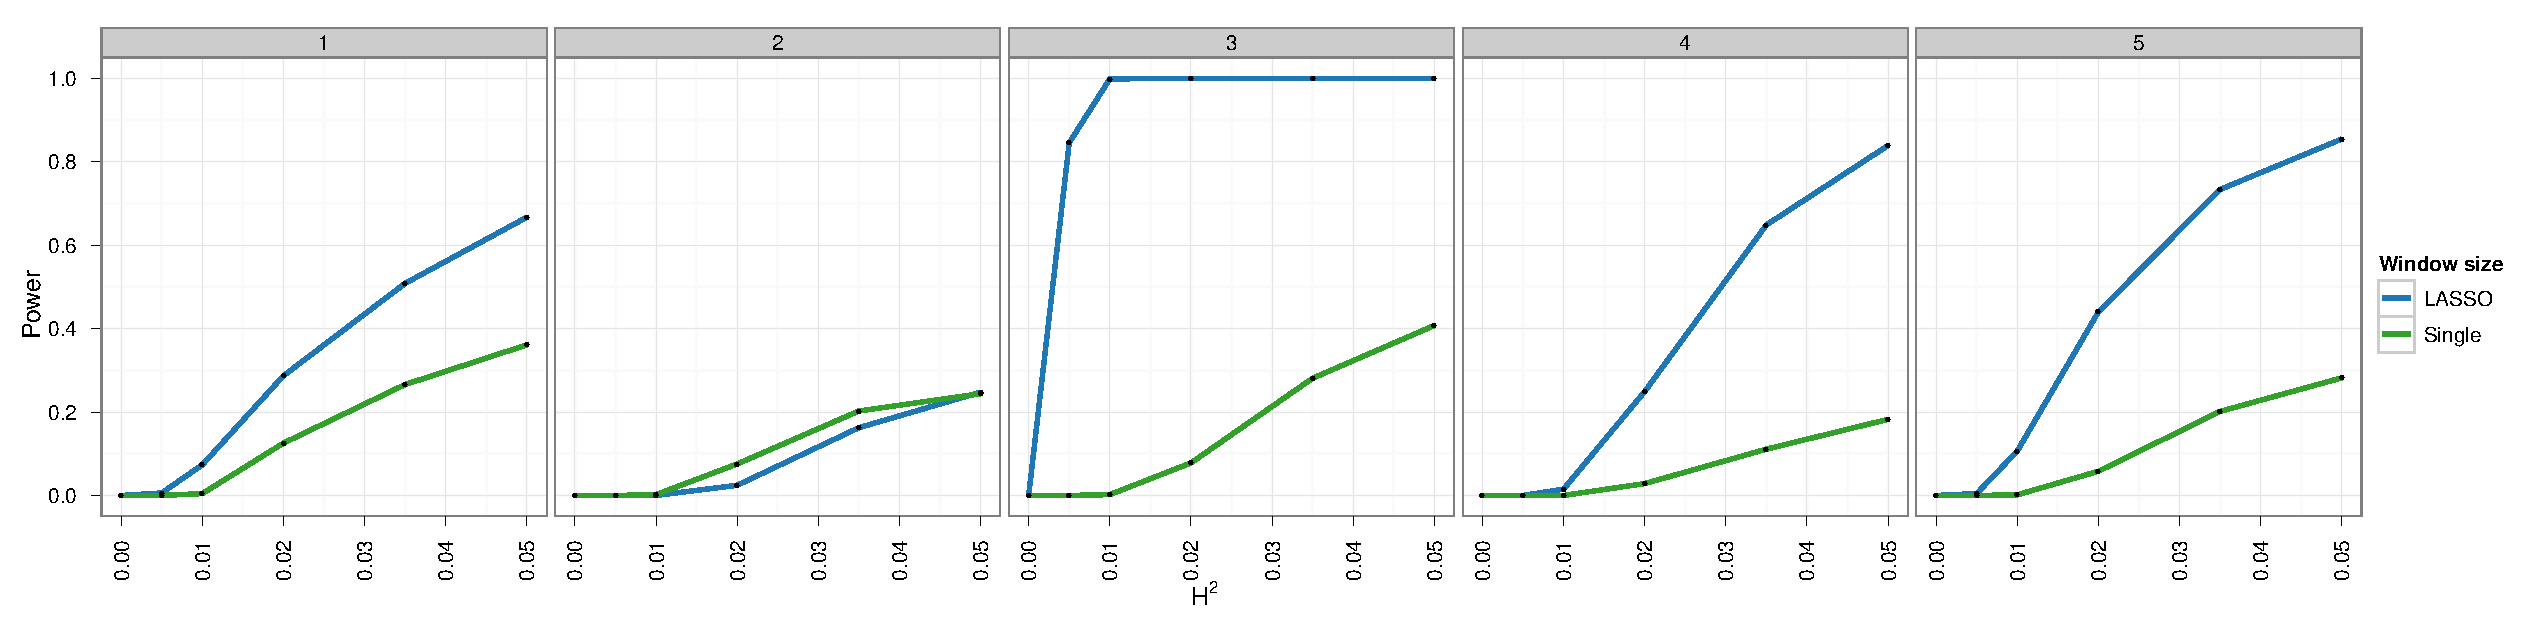
\includegraphics[width=5.5in]{Chapter4/power_bonferroni.pdf}} \\
\caption[Comparison of power between different scanning methods]{Comparison of power between different scanning methods (coloured lines) for each epistatic genotype-phenotype map (boxes correspond to first column of figure \ref{fig:gpmaps_ld}), where thresholds for (a) are calculated from false discovery rates, and for (b) from Bonferroni corrections corresponding to the SNP chip density. The results are for sample sizes of 4000 individuals. Power values are for overall power when amalgamating simulation results from all maximum QTL frequency parameters and effective SNP density parameters. Results are expanded to include these parameters in figure \ref{fig:power_methods_extended}.}
 \label{fig:power_methods}
\end{center}
\end{center}
\end{figure}


\paragraph{Effect of QTL frequency distribution on power}
The genetic variance simulated for each phenotype was not a function of the QTL frequencies, so any difference in performance for different frequencies must be a result of genomic architecture. Figure \ref{fig:power_methods_freq} shows a clear improvement for the single SNP method as the distribution of QTL frequencies becomes more closely matched to the distribution of frequencies in the SNP panel. This is logical, as theoretical $r^2$ values between causal variants and observed SNPs are maximised when the frequencies are equal, and increasingly limited as frequencies become more divergent \citep{Schork2000}. This is mostly the case for LASSO regression also, however the relationship is reversed for the $A \times A$ map. One possible explanation for this could be that lower frequencies could be favoured by diplotype methods as the frequencies of diplotypes are likely to be low also. Another observation that may have an impact is that at more intermediate frequencies the marginal effects in the model disappear, although it is unclear if or how this would be the underlying reason for the reduction in power as the parameterisation should be insensitive to this change.

\paragraph{Effect of SNP density on power}
An interesting paradox exists in searching for epistasis, in that as shown in figure \ref{fig:gpmaps_ld} and in chapter 2, there is a heavy dependence on high LD between causal variants and observed QTLs, however the usage of denser SNP chips to increase LD inevitably causes a steep increase in multiple testing corrections. This is reflected in figure \ref{fig:power_methods_density}, where increasing SNP chip density has very little improvement in power because it is offset by the increased multiple testing penalty imposed through a Bonferroni threshold.

\paragraph{Effect of sample size on power}
The improvement in power conferred by LASSO regression on diplotypes over single SNPs is mostly lost when the sample size is reduced to 1000 individuals when the average power across all $H^{2}$ is close to 0. The relationship between power and sample size is close to linear for both testing methods, however the improvement gained from LASSO is maximised when the sample size is greatest. In terms of experimental design it is of high importance to incorporate large sample sizes, the power to detect even reasonably large variants diminishing rapidly with sample sizes that may be considered reasonable for one dimensional scans.


\begin{figure}
\begin{center}
\begin{center}
\subfigure[QTL frequency]{\label{fig:power_methods_freq}\includegraphics[width=5.5in]{Chapter4/power_methods_freq.pdf}}
\subfigure[SNP chip density]{\label{fig:power_methods_density}\includegraphics[width=5.5in]{Chapter4/power_methods_density.pdf}}
\subfigure[Sample size]{\label{fig:power_N}\includegraphics[width=5.5in]{Chapter4/power_N.pdf}}
\caption[Power performance under different conditions]{Power performance with different maximum QTL frequencies (a), effective SNP chip densities (b), and sample sizes (c), using the Bonferroni threshold corresponding to the simulated SNP chip density. Boxes of graphs represent the genotype-phenotype maps in figure \ref{fig:gpmaps_ld}. Values are calculated by averaging across all simulated values of $H^{2}$.}
\label{fig:power_methods_extended}
\end{center}
\end{center}
\end{figure}


\section{Discussion}

% frequency bigger problem for LD than density
% trans interactions between cis interactions

There have been many successful attempts at improving the statistical power of detecting additive genetic variants by moving from genome-scans based on independent single markers, to those that test for associations with sliding windows of haplotypes. Yet although one could argue that applying such methods to epistasis is theoretically likely to offer an even greater improvement, no such methods currently exist in the literature. The advantages of using haplotypes are two fold, firstly they capture biologically functional units of inheritance, intrinsically considering \emph{cis}-epistatic relationships; and secondly they may capture the genotypic states of untyped causal variants more accurately if alternative alleles segregate among the haplotypes in a population. Only the latter case was investigated in the simulations in this study - the potential improvements made in capturing the variance of \emph{trans}-epistatic interactions - so while these results are fairly positive, even greater advantages could be gained when applying to real data, should combinations of \emph{cis}- and \emph{trans}-epistatic effects exist. 


\subsection{Unsupervised haplotype clustering}

Several clustering methods were proposed for adaptation to haplotype data in an epistatic context. Ultimately, none of those tested could be practicably applied with a gain in power over independent single SNPs. An hypothetical advantage in clustering haplotypes to biallelic vectors that would have been desirable is that, as shown in figure \ref{fig:gpmaps_ld}, if the correlation between the clustered vector and the causal variant is increased then the functional genotype-phenotype map is rescued. Unfortunately, although figure \ref{fig:best_scenario} shows promise due to the notion that in ideal circumstances often the extent to which the LD is rescued is high, the issue of being unable to predict window size in an unsupervised manner means that it is statistically impractical at this stage.

From figure \ref{fig:unsupervised_overall} the $k$-modes and cladistic methods appear to rival the single SNP method the closest, however when translating to figure \ref{fig:best_scenario}, where only the best window size is considered, the ROCK algorithm appears to offer the most advantage. This observation suggests that the correlation of clustered vectors between window sizes is very high, so considering each window size jointly does little to improve the predictability of the causal variant. However with the ROCK algorithm, although each window performs poorly independently, they are more lowly correlated and therefore when considered jointly have better predictive properties. 


\subsection{Supervised parameter reduction methods}

In contrast to the unsupervised methods, employing the LASSO to eliminate uninformative parameters from the population of haplotypes appears to result in a huge improvement in power over other both the haplotype regression methods, as well as the standard independent SNP method. The approach gains its power from performing a feature selection step that is regularised such that the false discovery rate doesn't become inflated, which would otherwise demand increasingly extreme $p$-values to be deemed significant. With many feature selection approaches, such as stepwise regression, it is inaccurate to simply count the parameters that remain in the model to ascertain the degrees of freedom to be used for hypothesis testing, because additional degrees of freedom have been used in selecting the subset of parameters that remain \citep{Hastie2009}. Calculating the effective number of degrees of freedom is difficult, and ultimately such an approach defeats the purpose of parameter reduction methods in this context. Conversely, it has been shown that the effective number of degrees of freedom in a feature subset obtained from the LASSO is approximately equal to the number of features that remain \citep{Zou2007}. This regularisation is achieved by shrinking the coefficients that remain non-zero in the model concomitant with the removal of uninformative parameters. The method developed in this study applied this approximation and through null-model simulations it can be shown that the false discovery rate is not inflated (figure \ref{fig:fdr} and table \ref{tab:thresholds}). 

So how does the LASSO gain its power if features are being regularised? One intuitive explanation concerns the evolutionary structure of haplotypes in the population. If the causal variant genotypes neatly segregate among a subset of the population's diplotypes, while the remaining diplotypes each harbour more than one genotype class of the causal variant, the estimated coefficients of these ambiguous diplotypes will invariably be smaller than the informative diplotypes, as mixed effects cause the class mean to tend towards the phenotype mean. Resultantly, they will be dropped rapidly from the model, allowing the informative diplotypes to remain. Because the matrix $V$ is a design matrix with unambiguous diplotype statehood, the correlation structure between parameters is very weak. Ordinarily with LASSO regression correlated parameters are rapidly paired down so that redundancy does not remain in the model. With no correlation between parameters this cannot be performed, which allows the possibility for the effects of a particular genotype class to be accounted for multiple times if alternative diplotypes harbour them simultaneously. Ultimately the feature subset will comprise many parameters, often more than the 9 parameters that comprise the independent single SNP model, but the coefficient of each parameter will be significantly different from the phenotype mean. Such an approach seems to neatly address the two locus diplotype's major statistical obstacle of having extremely high numbers of parameters.

This may be related to the reason that smaller sliding windows appear to be most powerful. While the use of larger window sizes will potentially comprise higher numbers of informative parameters, they will also include very many that are uninformative. Therefore, the shrinkage parameter will be increased in order to eliminate a larger proportion of the parameters, such that the increased number of informative parameters will be offset by the increased shrinkage of each parameter, while the number of degrees of freedom in the model will potentially increase.

The alternative approach to addressing this issue is to treat diplotype effects as random, rather than as fixed as in the LASSO. In terms of modelling it is perhaps more accurate to consider the diplotypes that exist in a window to be a random sample of all possible diplotypes that exist in the population, so the REML approach is justifiable. However, its performance was worse than all other methods, despite the statistical advantage of tests comprising only one degree of freedom (figure \ref{fig:power_methods_fdr}). A possible reason for this could be that variance estimates of rare diplotype classes become unstable, thus models may fail to converge even when they might otherwise have explained a significant proportion of the variance. It could be possible to overcome this problem quite simply by grouping rare classes together, or by employing a clustering step, and then performing random regression on the clusters.

Another problem may be that although the F-test's numerator degrees of freedom has been dealt with, the denominator degrees of freedom will often be significantly lower also, as in fixed effect tests this is a function of the number of observations, while in the case of random effects it is rather the number of parameters, thus weakening the test statistic. In addition, a recent simulation study \citep{Struchalin2010} concluded that while an increase in variance within genotype classes must necessarily be caused by some underlying interaction (with other genetic or environmental factors), interactions did not necessarily cause heterogeneity in variance. Thus the explicit test of testing for differences in means may intrinsically provide greater coverage of all possible interaction scenarios than a variance based metric such as the REML method used here.


\subsection{Effects of genomic architecture}

Of interest is how best to design the genome-wide association scan in terms of SNP chip density and number of individuals under varying assumptions of the architecture of the causal variants. Perhaps the most obvious observation is that sample size should be maximised (figure \ref{fig:power_N}), natural advice with all large $p$ small $n$ problems. These simulations show that none of the approaches were particularly robust to diminishing sample size, and that indeed relatively high numbers (\emph{i.e.} 4000 individuals) were required to achieve even modest power levels. An interesting observation is that in most situations the LASSO method lost power more rapidly than the independent single SNP method. This is likely due to the fact that a very large number of parameters per test are more heavily dependent on a large sample size in order to reduce standard errors on coefficient estimates, with the problem accelerating faster as sample size drops than when there are relatively few parameters as in the independent single SNP method.

A second problem that is of concern for searching for epistasis is that of SNP chip density. Being heavily reliant upon high LD will likely encourage the use of denser SNP chips, but figure \ref{fig:power_methods_density} shows quite neatly that on average any gain in variance is offset by elevated multiple testing penalties. This paradox is difficult to reconcile in practice. From the perspective of haplotype methodology, at least in one dimensional scans, if the LD between causal variants and observed SNPs is on average very high (\emph{e.g.} very dense SNP panels or sequence data) then single SNP methods will generally be more powerful. If the LD is very low on the other hand then haplotypes become excessively noisy, with high recombination rates destroying any QTL segregation structures, and again single SNPs will be more powerful, although neither method will be especially powerful. Haplotype methods are strongest somewhere in the middle of this LD continuum, where single SNPs generally have loose correlations with the causal variants. With epistasis, because the genetic variance decay is so much more rapid (figure \ref{fig:gpmaps_ld} and chapter 2), the range of this middle ground is likely to be larger than in the additive case. The simulations performed look at the density range of 100000 SNPs to 700000 SNPs, it is possible that if this were extended to more extreme values then relative differences between haplotype and independent SNP methods will manifest.

Thirdly, it is prudent to ask how underlying causal variant frequency distributions will inform experimental design. As shown by \citet{Schork2000} the level of LD that can be achieved between two SNPs is highly dependent upon the similarity of their allele frequencies, so if the distribution of observed SNP frequencies is particularly disparate from that of causal variants then single SNP effects will suffer. From the unsupervised methods approach, the ROCK algorithm shows that there is a strong relationship between its benefit over single SNPs and the maximum frequency of QTLs simulated (figure \ref{fig:best_scenario}), and indeed this has also been reported in several other studies (\emph{e.g.} \citealp{Durrant2004}; \citealp{Browning2007}; \citealp{Schaid2004}). This is likely to do with the occurrence of low frequency haplotypes that can accurately segregate with low frequency QTLs. Interestingly, only in one of the five epistatic patterns echoed this result in the comparison between LASSO and single SNP methods (figure \ref{fig:power_methods_freq}). For the remaining four patterns, both methods performed worse as maximum QTL frequency declined, however for $A \times A$ the improvement in power of LASSO over single SNPs increased. Interestingly, \citet{Yang2010} showed that the observation that heritability estimates obtained from genomic relationships based on SNP chips are generally lower than those made from pedigree relationships could be attributed to the common situation where QTLs generally have much lower frequencies than the SNPs in a marker panel. Poor genome-wide association results could similarly be attributed to this, and haplotype methods have been advocated to overcome this in the additive case. From these simulations the advantage of diplotypes at low frequencies is not so consistent, however they may still confer some advantages.

A note of caution should also be made. Though designed to mimic the construction of populations of genomes in an evolutionarily realistic manner \citep{Hoggart2007}, it is difficult to faithfully recreate the more chaotic haplotype structure that might exist given the rather ``noisy" LD patterns found in real data using deterministic simulations. This is one reason that translating these simulations to real data might result in less impressive results for the LASSO method. Another reason is that unlike in the case of simulated data perfect phase will be unknown, as real data is unlikely to be completely informative at every locus for methods such as long range phasing \citep{Kong2008}.

Though this is the first application of LASSO to haplotype parameter reduction in for a quantitative response variable, methods have been previously described that employ a logit function to a binary response variable (case/control disease status). In the one dimensional additive case \citet{Guo2009} demonstrated that while an improvement in power over single SNPs could be made with common variants, the most benefit was achieved for detecting rare variants. Conversely, \citet{Li2010} found that the application of this approach to $2 \times 2$ window diplotypes in the epistatic case was not as powerful as single markers. One potential reason for this could be that they use an EM algorithm to derive phase, thus resulting in a quantitative predictor matrix with intrinsic correlation structures, and multi-collinearity causing a reduction in the total variance explained following elimination during the parameter reduction step.


\subsection{Computational viability}

As demonstrated in chapters 3 and 4, the computational viability of exhaustive two dimensional scans is now a reality. Problems arise, however, when the kernel being parallelised becomes more sophisticated, as in LASSO regression. From the simulations performed here, there was generally a rapid decline in computational speed as the window sizes increased from $2 \times 2$ to $6 \times 6$ by many orders of magnitude. In terms of statistical benefits one would naturally recommend the LASSO regression on $2 \times 2$ window diplotypes over independent single SNPs, but whereas single SNP regressions and F-tests can be performed in the order of 128000 per second on a single CPU (chapter 3), the computational performance according to these simulations suggest that LASSO regression will achieve only 30-40 tests per second (depending on the number of parameters). For an exhaustive scan on a 100000 SNP chip, this would require at best $\sim 1500$ CPU days. This is perhaps tractable with access to a large compute cluster, and further speed improvements can be made, because although the main computational task of coefficient estimation performed using the {\tt R/glmnet} package is highly efficient, having been written and optimised in FORTRAN \citep{Friedman2010}, the simulation framework, diplotype parameter construction, and test statistic calculation were performed in R.

An alternative approach, although less statistically desirable, could be to consider using single two stages. For example efficient single SNP methods could be used to identify candidate regions based on a relaxed threshold in a two dimensional setting in an initial stage, with LASSO regression being applied to interesting regions in the second stage. By contrast, a haplotype or diplotype method could be implemented in a one dimensional scan with the regions of interest being forwarded to a two dimensional diplotype scan.


\chapter{Discussion}
\label{Discussion}
\lhead{Chapter 5. \emph{Discussion}}


\section{Objectives}

After being predicated on a largely additive statistical paradigm, the disappointing results of large scale genome wide association studies over the last decade have caused the architecture of natural genetic variance to come into question \citep{Eichler2010}. Epistasis has an established place in population and quantitative genetic theory, yet since the advent of GWAS it has been largely neglected from empirical exploration. There have been three major reasons for this. Firstly, estimates of genetic components have frequently suggested that there is little statistical contribution from non-additive effects \citep{Hill2008a}. Secondly, with the acceleration in genotyping technology the computational barrier of searching for genetic interactions soon became insurmountable with standard programming techniques. And thirdly, while the statistical power to detect small independent effects is already low, the problem becomes considerably more acute when extending the search to interactions.

This thesis has attempted to address each of these issues. To briefly summarise, it was shown that the maintenance of additive variation in fitness related traits can be achieved through epistatic interactions, and that the presence of additive variance may in fact be symptomatic of a more complex genomic architecture. The computational challenges of searching for these interactions exhaustively were mitigated through the use of an emerging form of parallel programming based on cheap, consumer level graphics cards. Indeed the performance of these devices is such that if using CPUs, the permutation experiments performed in chapter 4 will have taken up to 200 compute years, but with the availability of modestly sized GPGPU clusters this was completed in a few months of user time. Finally, it was attempted to address some of the statistical challenges by parameterising SNP data as haplotypes in order to rescue the LD with unobserved causal variants, and through extensive simulations it can be shown that when combined with penalised regression techniques this can effect a significant improvement in statistical power.


\section{Further considerations}

\subsection{Higher order interactions}

The work presented here considers epistasis only from a fairly narrow perspective - that of two locus interactions. The computational challenge of searching exhaustively in 3 dimensions or more is currently insurmountable with the density of marker information required to adequately capture the variance of untyped causal variants, and perhaps more to the point the tractability of exhaustive searching from a statistical point of view is questionable, both in terms of the significance thresholds required and the potential combinatorial problems that were discussed in chapter 4.

It may be the case that searching in higher than two dimensions is not necessary. For example, the discovery of epistatic networks involving many loci can be made from two dimensional searches alone (\emph{e.g.} \citet{Carlborg2006}), and just as independent SNPs can explain some of the variance of their joint effects, it would be interesting to explore how much of the variance of higher order interactions can be explained marginally in two dimensions.

The evolutionary properties of higher order interactions are also difficult to predict, in particular it may be the case that higher order interactions maintain additive variance more effectively than the two locus interactions explored in chapter 2. Should this be the case then it may be of practical importance to understand how best to map such genetic factors. One potential approach could be to test for variance heterogeneity within loci. While it has been shown that this is not as powerful for detecting two locus interactions as the direct method of treating them as fixed effects \citep{Struchalin2010}, the behaviour with regards to higher order interactions is unknown. 


\subsection{Phenomics}

The number of genetic factors, or the polygenicity, governing heritable traits is fairly variable. For example, susceptibility to infectious disease is speculated to be under the control of relatively few polymorphisms with large effects \citep{Min-Oo2003, Diez2003}, while other traits such as height, obesity, and red blood cell count appear to be much more in the dominion of the infinitesimal model \citep{Valdar2006, Park2010}, being controlled by very many variants of small effects. One approach that is used to overcome the problem of high polygenicity is to expand the sample size of the study. Perhaps the most extreme example of this to date is the meta-analysis of human height performed by \citet{LangoAllen2010} which included over 180000 individuals in total. While this was effective at detecting many variants ($>180$), the proportion of phenotypic variance explained remained fairly low at around 10\% overall.

To generalise, it could be said that the set of predictor variables in a GWAS, the fixed genetic effects, are extremely well characterised, while the response variable is rarely anything more than a single binary or quantitative variable. Perhaps a more effective way to overcome high polygenicity would be to redress this balance through the inclusion of large-scale phenotyping (``phenomics", \citet{Sabb2009, Houle2010}). The argument for this approach is that one reason that high level disease phenotypes are so polygenic is that they are the manifestation of many different lower level phenotypes. If these lower level phenotypes are less polygenic then mapping genetic variation to them may be more statistically tractable. Thus an overall understanding of the genetic components contributing to high level disease trait of interest could then be composed by reconstructing the relationships between lower level phenotypes.

Some success has already been achieved with this type of approach. For example expression QTL (eQTL) studies that aim to map genetic variation to variation in gene expression levels, arguably a very low level phenotype, tend to uncover extremely large effect sizes relative to the higher level morphological phenotypes that are more commonly used in GWAS. Resultantly, high proportions of the variance of expression can be detected with relatively modest sample sizes \citep{Bystrykh2005, Cookson2009}. Typically these types of studies are restricted to searching for additive \emph{cis}-QTLs and it is uncommon to extend the analysis to include genome-wide epistasis, thus there is potential for these types of studies to expand in scope and begin to assay the underlying architecture of genetic variation.

While the use of lower level phenotypes has the potential to overcome the problems associated with the infinitesimal model, employing such an approach in an integrative phenomics model may have its own set of problems. High throughput phenotyping is currently possible for gene expression, proteomic and metabolic data, but the question of implementation is still difficult. For example, a realistic assay of the phenome might involve the collection of this type of data from multiple tissues at several time points. Aside from being potentially invasive, this is most likely financially prohibitive. In addition, from a statistical point of view the problem of causality emerges. When constructing relationships between low level phenotypes, assigning directionality to the effects in a network is difficult \citep{Shipley2000}, and this may be very limiting for prediction accuracy. For example which low level phenotypes are upstream of the manifestation of disease (causative), which are downstream (consequential), and which are simply confounded? Theoretically it is only the upstream events that will have predictive value for the outcome of disease phenotypes \citep{Shipley2000} and uncovering correlations alone in the phenome will be insufficient for a realistic prediction model.


\subsection{Threshold based searches}

Though the broad goal is to identify causal variants, GWAS in its standard form is generally only concerned with identifying regions of association. The question of the direction of causality in genetic associations is undisputed, logically phenotypes cannot `cause' a genetic variant. This is an uncommon feature in data mining in general, the inference of causality often being difficult to ascertain in most statistical frameworks. However the belief that the variant has a real biological association is disputable, even after surpassing the stringent family-wise testing thresholds that are routinely employed. Indeed, the philosophical question of what level of evidence is sufficient in order to be confident that a variant has a true biological effect is difficult to answer. But it should be clear that in the context of complex traits, where many effects contribute to the genetic variance, and each effect is supposedly small, statistical association in a single study alone is insufficient.

One approach to validating a candidate signal is to search for the same effect in an independent population and this is often a requirement for publication, although commonly the threshold for replication is relaxed. For example, \citet{Siontis2010} showed that in a survey of 291 candidate SNPs, only 41 were replicated with $p$-value $< 10^{-7}$, and the Catalog of Published Genome-Wide Association Studies \citep{Hindorff2010}, comprises 5845 significant associations, of which 2589 have not demonstrated any replication, and the median association $p$-value of ($1\times10^{-7}$) is below the widely suggested comparison-wise threshold of $7.2\times10^{-8}$ \citep{Dudbridge2008}. Even more extreme, \citet{Hirschhorn2002} surveyed 166 variants that had been studied in three populations, and found that only 6 were consistently replicated. Indeed \citet{Liu2008} demonstrated that the probability of replication across multiple independent populations is very small when power of detection is not close to 1, even in the simplest case where the true variant is purely additive.

Compounding the difficulty of replication, \citet{Greene2009} suggested that this problem is exacerbated further if the marginal effect is involved in a pairwise interaction. The marginal effects of two locus interactions for functional genotype-phenotype map tend to be highly dependent upon allele frequencies, and allele frequencies are liable to fluctuate across populations. Thus, it can be argued that searching for marginal effects alone will fail to replicate from one population to the next if they are involved in an interaction. \citet{Greene2009} went on to suggest that two-dimensional searches would alleviate this problem, and while this is true to some extent it also introduces other potential complexities. First, power to detect epistatic interactions is generally lower than marginal effects, so the problem of statistical replication, even with knowledge of the true interaction terms, will be inflated. Second, extrapolating their argument, the two-dimensional effects may be marginal to higher order interactions, in which case they are liable to the same fluctuations in allele frequencies across populations as are independent effects. And third, the interaction may be with environmental factors rather than other genetic loci, and this is a very complicated problem to control when comparing different populations.

In addition to these problems there are of course others. For example the initial association may be in LD with the true causal variant in one population but not the other, or the causal variant may simply not be segregating in other populations. Less stringent definitions for what constitutes a replication could be made with regards to this. For example, replication could entail searching for the same effect across all SNPs covering the same gene, all SNPs covering genes involved in the same pathway, or including the same gene ontology (GO) terms \citep{Cantor2010}. If robust statistical corrections are made for the increased multiple testing then this could ostensibly improve the power of detecting genomic regions with relevant functions, however such an approach does depart from the original problem of understanding genetic variation because without validating a candidate variant then the estimate for its mode of action remains unconfirmed. As discussed in chapter 5, the problems associated with incomplete LD will tend to inflate the importance of additive effects.

True variants are demonstrably difficult to replicate, but there is still some concern as to whether replication is in itself a strong foundation for belief of biological function as it can be shown that the probability of replication of a false positive can be fairly high under certain situations \citep{Liu2008}. Consequently, replication in independent populations, while commonly considered the gold standard of statistical association, probably still does not go far enough to address the question of true biological effect. \citet{Chanock2007} suggests that the more laborious procedure of candidate interval sequencing and genotyping of all regional common and uncommon variants in multiple populations should also be performed, followed by examination of functional consequences, and gene and environment interaction effects. Of course functional effects \emph{in situ} may be different from those examined in laboratory conditions, and there is no easy way to comprehensively measure the environmental conditions that may be involved. Further, under these guidelines the dissection of even a single variant is likely to be time consuming and costly, and ascertaining such levels of confidence for all variants associated with highly polygenic traits is a daunting task.


\subsection{Genetic prediction}

Alternative approaches exist that simply bypass the problem of stringent thresholds. The discovery of causal variants is important for two major reasons. First, it pinpoints areas of the genome that are functionally related to a phenotype of interest. Second, one can use this information to predict phenotypic outcomes. While epistasis may be important in the first instance in order to detect the causal variant and to understand the context in which the function occurs, its significance in the second instance may manifest in terms of the accuracy of the prediction.

In animal and crop breeding, where a principle objective is to select individuals with the most beneficial characteristics for genetic contributions to future generations, genomic selection has dominated quantitative genetic theory over the past decade. Whereas GWAS treats each SNP independently as fixed effects, genomic selection attempts to fit all genetic factors simultaneously as random effects in order to estimate the genomic breeding value (GEBV) of each individual \citep{Meuwissen2001}. This can be achieved through many methods \citep{Gianola2009}. Though no single approach is currently deemed superior above all others, particularly popular are those that parameterise all effects as additive and then use Bayesian sampling techniques in conjunction with highly sparse prior distributions for the variances of all loci. Here, the identification of individual factors or regions is largely inconsequential, and thus problems involving stringent thresholds are not relevant. Ultimately, genomic selection has been fairly successful, improving upon methods that involved progeny testing and delivering improved commercial productivity. For example, the accuracy of GEBVs in dairy cattle for milk yield are around 67\%, close to twice the accuracy of traditional pedigree-derived breeding values \citep{Harris2008}, and genotyping of elite animals is now becoming routine \citep{Hayes2009}.

Perhaps these types of studies can provide clues as to the statistical importance of epistasis. For example, if functional epistasis is prevalent amongst causal variants for milk yield, but prediction accuracy remains high with an additive parameterisation then this may suggest that interaction terms make a relatively small contribution to the variance, however without knowing the performance of such models in the hypothetical case that there are only epistatic terms contributing to the variance it is difficult to form any strong conclusions. Perhaps one can also use the results from genomic selection to begin to ascertain the polygenicity of a trait. A recent study attempted to apply genomic selection techniques for prediction in human height \citep{Makowsky2011}. For this trait, the REML estimate of the variance explained by the additive genomic relationship matrix was approximately 45\% \citep{Yang2010}, but both BLUP and Bayesian LASSO estimates, when 10-fold cross validated, resulted in an average prediction accuracy of less that 15\%. It has been shown for an additive polygenic model that the accuracy of prediction $r_{g\hat{g}}^{2}$ is constrained by the ratio of number of individuals $n_{p}$ to the number of causal loci $n_{G}$ and the observed heritability $h^{2}$ \citep{Daetwyler2008}:
\begin{equation}
r_{g\hat{g}} = \sqrt{\frac{\frac{n_{p}}{n_{G}}h^{2}}{\frac{n_{p}}{n_{G}}h^{2}  + 1}}.
\label{eq:daetwyler}
\end{equation}
One interpretation of the poor performance in prediction could simply be that the trait is highly polygenic. The study comprised 1493 individuals in the training set, so rearranging equation \ref{eq:daetwyler} to $n_{G} = r_{g\bar{g}}^{-2}(n_{p}h^{2} - n_{p}h^{2}r_{g\bar{g}}^{2})$ gives an estimated $n_{G} = 3807$. Given that the training and testing sets were from the same population and the prediction was based on cross validation one might expect that any systematic errors arising from interaction between genetic or environmental factors might be minimised. Thus, applying the estimated prediction model to other populations, where environmental conditions and allele frequencies will differ, may provide insight into the prevalence of interactions: if accuracy remains at 15\% then the most effective way forward for this particular trait would be to increase sample size, but if the accuracy drops then the genetic model may require revision.

Assuming that the inclusion of epistatic components will improve this type of study it still remains unclear how they might be incorporated into the prediction model. For example, one approach might be to simply obtain estimates based on the interacting pairs uncovered from two dimensional GWAS, however the variance explained of all significant factors combined would need to be high in order to achieve any reasonable level of accuracy \citep{Wray2007, Evans2009}. Alternatively a relaxed threshold could be used to allow a larger number of features with small effects to be utilised for prediction. However this has previously offered only small advantages in prediction for highly heritable traits such as schizophrenia \citep{Purcell2009}. Several methods have been proposed that could include non-additive variance components directly \citep{Gianola2006, Gianola2009, deLosCampos2009} and if the numerical difficulties associated with their estimation from genomic relationship matrices may be overcome with larger sample sizes then this may be an interesting direction to explore the global statistical impact of non-additive terms.


\section{Final remarks}

That high level morphological characters are manifested by the combination of discrete Mendelian processes implies an underlying granularity to the observed noisiness of biological systems, and GWA style approaches attempt to dissect this directly. But perhaps this is an overly simplistic representation, as stochasticity is likely to exist at every level higher than the genetic factors themselves, and it appears that overcoming this problem cannot be achieved without compromise. Genomic selection techniques sacrifice detail for prediction accuracy, whereas migrating GWAS to lower level phenotypes will sacrifice prediction accuracy for detail, and reconciling both approaches is evidently not straightforward.

There are a wide range of opinions as to the reasons behind the problem of the missing heritability \citep{Eichler2010}. While all valid, many of them are rather esoteric, invoking such concepts as the rare variant hypothesis, copy number variations, genetic imprinting, and non-additive genetic variance. But perhaps the most immediate problem is that with highly polygenic traits there is no strong basis to reject (or accept) the common disease-common variant hypothesis or the additive genetic paradigm. It might be argued that for the purposes of understanding the architecture of genetic variation genomic selection approaches are fairly subjective in terms of statistical interpretation. On the other hand, integrating a phenomic approach into the GWA framework has clear advantages for improving statistical power, and if the associated problems of causality can be addressed (\emph{e.g.} intsrumental variables \citet{McKeigue2010}), then one might speculate that both detailed functional information as well as good prediction accuracy could be obtained from genomic information.

Additive parameterisations have dominated the data mining techniques for causal genetic polymorphisms in recent years but the question of the type of genetic variance that underlies complex traits remains an important one to resolve. It is unlikely that a single solution exists, and the architecture of one trait may be entirely different to the architecture of another. Ultimately, epistasis may or may not have an important role in complex traits, but a theoretical precedence for it has long been established. Today, the necessary data is abundant and the data mining tools have been developed, so the true importance of epistasis can now begin to be qualified empirically.





\appendix




\chapter{Further analysis of epistasis under selection on extended set of patterns}
\label{AppendixA}
\lhead{Appendix A. \emph{Epistasis under selection}}

\begin{figure}
\begin{center}
\includegraphics[scale=0.65]{Chapter1/sup_gpmaps.pdf}
\caption[Extended set of genotype-phenotype maps]{Extended set of genotype phenotype maps. \emph{1} Neutral; \emph{2-51} Enumeration of all binary trait patterns, excluding reflections, rotations and inversions, as derived by \citet{Li2000} (6 and 29 are non-episatatic); \emph{52-56} Additive x Additive, Additive x Dominance, Dominance x Dominance, Over-dominance, additive.}
\label{fig:sup_gpmaps}
\end{center}
\end{figure}

\begin{figure}
\begin{center}
\includegraphics[scale=0.6]{Chapter1/sup_allelefreq_det.png}
\caption[Deterministic trajectory of allele frequencies for extended maps]{Deterministic trajectory of allele frequencies as in figure \ref{fig:allelefreq_det}, but for an extended set of patterns (detailed in figure \ref{fig:sup_gpmaps})}
\label{fig:sup_allelefreq_det}
\end{center}
\end{figure}

\begin{figure}
\begin{center}
\includegraphics[scale=0.6]{Chapter1/sup_allelefreq_sim.png}
\caption[Simulated trajectory of allele frequencies for extended maps for extended maps]{Simulated trajectory of allele frequencies as in figure \ref{fig:allelefreq_sim}, but for an extended set of patterns (detailed in figure \ref{fig:sup_gpmaps})}
\label{fig:sup_allelefreq_sim}
\end{center}
\end{figure}

\begin{figure}
\begin{center}
\includegraphics[scale=0.6]{Chapter1/sup_r_det.png}
\caption[Deterministic calculations of quasi-LD for extended maps]{For the 25 deterministic simulations the expected quasi-LD between the physically unlinked causal SNPs was calculated. It can be seen that significant levels are generated, such that orthogonal standard parameterisation methods would not be orthogonal. Boxes represent different genotype-phenotype maps from figure \ref{fig:sup_gpmaps}.}
\label{fig:sup_r_det}
\end{center}
\end{figure}

\begin{figure}
\begin{center}
\includegraphics[scale=0.6]{Chapter1/sup_Vg_det.png} \\
\caption[Deterministically calculated change in genetic variance for extended maps]{Deterministic change in genetic variance for loci under selection exhibiting various epistatic patterns (figure \ref{fig:sup_gpmaps}), when LD between the causal variants and observed SNPs varies. For clarity, only the results from initial frequencies of 0.5 at both loci are shown. Boxes represent different genotype-phenotype maps from figure \ref{fig:sup_gpmaps}.}
\label{fig:sup_Vg_det}
\end{center}
\end{figure}

\begin{figure}
\begin{center}
\includegraphics[scale=0.6]{Chapter1/sup_propadditive_det.png} \\
\caption[Deterministically calculated change in additive variance for extended maps]{As in figure \ref{fig:sup_Vg_det}, but this time showing the proportion of the genetic variance that is additive.}
\label{fig:sup_propadditive_det}
\end{center}
\end{figure}

\begin{figure}
\begin{center}
\includegraphics[scale=0.6]{Chapter1/sup_heritbars_sim.png} \\
\caption[Proportion of additive variance detected for extended maps]{As in figure \ref{fig:heritbars_det}, but for only three tests - Additive in one dimension (A (1D)), genotype in one dimension (A+D (1D)), and full epistatic in two dimensions (F (2D)). Each box has the additive variance detected across all populations and generations as a proportion of the total additive variance that was created for each test when the observed SNPs were in varying levels of LD with the causal variants. For 44 patterns the full epistatic test is most powerful when $r^{2}=1$, but when $r^{2} = 0.7$ it is never the most powerful, rather 39 patterns are best detected by the one dimensional genotype parameterisation}
\label{fig:sup_heritbars_det}
\end{center}
\end{figure}



\backmatter

\setstretch{1}
\label{Bibliography} \lhead{\emph{Bibliography}}
\bibliographystyle{natbib}
\bibliography{thesis}
\end{document}
